\documentclass[12pt]{article}
\usepackage{amssymb,amsmath,amsthm}
\usepackage[mathscr]{eucal}
\usepackage{graphics}
\usepackage[dvips]{graphicx}
\usepackage{epsfig}
\usepackage{easybmat}
\DeclareGraphicsExtensions{.pdf,.png,.jpg}
\graphicspath{{pictures/}}
\makeatletter
\renewcommand*\env@matrix[1][c]{\hskip -\arraycolsep
  \let\@ifnextchar\new@ifnextchar
  \array{*\c@MaxMatrixCols #1}}
\makeatother
\usepackage{wrapfig}
\usepackage{enumitem}

\usepackage{indentfirst,float,cite}
%comment!!! \usepackage[cp1251]{inputenc}
\usepackage[utf8]{inputenc}
\usepackage[T2A]{fontenc}
\usepackage[english]{babel}

%\usepackage{showlabels}
%!!!\usepackage{showkeys}

%\documentclass[12pt,a4paper]{article}
%\usepackage{indentfirst,amssymb,amsmath,amsthm,float,cite}
%\usepackage[dvips]{graphicx}
%\usepackage[cp1251]{inputenc}
%\usepackage[T2A]{fontenc}
%\usepackage[russian]{babel}


\oddsidemargin 0in
\evensidemargin 0in
\topmargin -0.5in
\textwidth 16.5truecm
\textheight 23truecm

\parindent=18pt

\newcommand{\comment}[1]{}
\newcommand{\e}{\varepsilon}
\newcommand{\eps}{\epsilon}
\newcommand{\nc}{\newcommand}
\nc{\re}{\mathrm{e}}
\nc{\ls}{\leqslant}
\nc{\pa}{\partial}
\nc{\al}{\alpha}
\nc{\dt}{\delta}
\nc{\la}{\lambda}
\nc{\ve}{\varepsilon}
\nc{\ph}{\varphi}
\nc{\td}{\tilde}
\nc{\wt}{\widetilde}
\nc{\lb}{\linebreak}
\nc{\intl}{\int\limits}
\nc{\intlzt}{\intl_0^t}
\nc{\intlzinf}{\intl_0^\infty}
\nc{\intlinf}{\intl_{-\infty}^{+\infty}}
\nc{\suml}{\sum\limits}

\newcommand{\BL}{\biggl}
\newcommand{\BR}{\biggr}
\newcommand{\Bl}{\Bigl}
\newcommand{\Br}{\Bigr}
\newcommand{\bl}{\bigl}
\newcommand{\br}{\bigr}

\def\gN{{\mathfrak{N}}}
\def\gS{{\mathfrak{S}}}



\newtheorem{lem}{Lemma}
\newtheorem{lemma}{Lemma}
\newtheorem{lemma*}{Lemma}
\newtheorem{remark}{Remark}
\newtheorem{theorem}{Theorem}
\newtheorem{exlem}{Lemma}
\newtheorem{prop}{Proposition}
\newtheorem*{cor*}{Corollary}
\newtheorem*{corollary}{Corollary}
\theoremstyle{definition}
\newtheorem{example}{Example}
\newtheorem{exampleA}{Example}
\newtheorem*{example*}{Example}
\newtheorem*{rem*}{Remark}
\newtheorem{Fig}{Fig.}
\numberwithin{equation}{section}
\renewcommand{\theequation}{\arabic{section}.\arabic{equation}}
\renewcommand{\theexampleA}{A\arabic{exampleA}}

\makeatletter
%------------
\renewcommand{\@seccntformat}[1]{\csname #1name\endcsname\csname the#1\endcsname.\quad}
%------------
\renewcommand{\@biblabel}[1]{#1.}
%------------
\def\@Scaptionlabeldelim{.}
\def\@Ssize{\small}
\def\@Sshape{\upshape}
\def\@Sseries{\mdseries}
\def\@Sfamily{\rmfamily}
\long\def\@Smakecaption#1{%
  \vskip\abovecaptionskip
  \sbox\@tempboxa{\@Sshape\@Sseries\@Sfamily #1.}%
  \ifdim \wd\@tempboxa >\hsize
    {\@Stshape\@Stseries\@Stfamily #1.}\par
  \else
    \global \@minipagefalse
    \hb@xt@\hsize{\hfil\box\@tempboxa\hfil}%
  \fi
  \vskip\belowcaptionskip}
\def\Scaption{\refstepcounter\@captype\@Scaption\@captype}
\long\def\@Scaption#1{\par\addcontentsline{\csname
  ext@#1\endcsname}{#1}{\protect\numberline{\csname
  the#1\endcsname}}\begingroup
    \@parboxrestore
    \@Ssize
    \@Smakecaption{\csname fnum@#1\endcsname}\par
  \endgroup}
%------------
\makeatother

\pagestyle{plain}
%\usepackage{showkeys}
\begin{document}
\title{Прикладные проблемы линейной алгебры}
\date{}
\maketitle \sloppy


\section *{Лекция 1}
\noindent \textbf{Псевдообратная матрица.}\\\\
Пусть имеется СЛУ
$$Ax=b$$
Тогда если $\exists A^{-1}$, то $x=A^{-1}b$.\\
\\
Так как часто матрица является вырожденной или неквадратной, появляется необходимость ввести обобщение обратной матрицы.\\
\\
Псевдообратная матрица $A^+$ позволяет найти решение через явную формулу $x=A^+b$ для любой матрицы $A$, если оно существует. Если решения нет, то $x=A^+b$ будет наилучшим приближенным решением по евклидовой метрике, то есть, расстояние между $Ax$ и $b$ будет минимальным.\\\\
\noindent \textbf{Определение.}\\\\
$C=A^+$ (где $C_{n \times m}, ~A_{m \times n})$ --- \textbf{псевдообратная матрица Мура-Пенроуза} для матрицы $A$, если:
\begin{enumerate}
\item $ACA=A$
\item $CAC=C$
\item $(AC)^*=AC=C^*A^*$
\item $(CA)^*=CA$
\end{enumerate}
\[\begin{pmatrix}
1+i & 3-i\\
2i & 5\\
\end{pmatrix}^* = \begin{pmatrix}
1-i & -2i\\
3+i & 5\\
\end{pmatrix}\]
\\ 
Если $detA \neq 0$, то подходит $C=A^{-1}$.\\
\\
\textbf{Теорема 1.}
Если такая матрица $C$ существует, то она единственная.\\
$\blacktriangleright$ Пусть $B, C$ --- две матрицы, удовлетворяющие свойствам 1 - 4.\\
$$AB\overset{1}{=}\underbrace{ACA}_{A}B=(AC)(AB)\overset{3}{=}(AC)^*(AB)^*=C^*A^*B^*A^*=$$
$$=C^*(ABA)^*\overset{1}{=}C^*A^*=(AC)^*\overset{3}{=}AC$$\\
Аналогично выводится $BA=CA$. Тогда
$$B\overset{2}{=}BAB=\underbrace{BA}_{CA}B=C\underbrace{AB}_{AC}=CAC\overset{2}{=}C$$\\
Значит, $B=C$, то есть, псевдообратная матрица единственна. $\blacksquare$\\ \\
\noindent \textbf{Пример 1.}\\
Найти псевдообратную матрицу.\\ \\
\[\begin{pmatrix}
1 & 0 & \cdots & 0 \\
0 & 0 & \cdots & 0 \\         
\vdots & \vdots & \ddots & \vdots \\
0 & 0 & \cdots & 0
\end{pmatrix}^+ = \begin{pmatrix}
1 & 0 & \cdots & 0 \\
0 & 0 & \cdots & 0 \\         
\vdots & \vdots & \ddots & \vdots \\
0 & 0 & \cdots & 0
\end{pmatrix}\]\\
$
\left\{ 
\begin{array}{ll}  
    AA=A \Rightarrow A=A^+\\
    A^*=A\\
\end{array}   
\right.
$\\ \\
\noindent Мы доказали единственность, значит другая матрица не подойдет.\\ \\
$O_{m \times n}^+ = O_{n \times m}$\\
\[ A_{m \times n}=\bordermatrix{
&r  & n \cr
r & X_{r \times r} & O \cr 
m & O & O \cr } , ~ A_{n \times m}^+=\bordermatrix{
&r  & m \cr
r & X_{r \times r}^+ & O \cr
n & O & O \cr }\]\\
\textbf{Пример 2.}\\
Найти $A^+$.
\[A=\begin{pmatrix}
a_1 \\
\vdots \\         
a_n
\end{pmatrix}\]\\
$A^+=(b_1 \cdots b_n), ~ b_1,...,b_n$ - ?\\ \\
Из свойств получим:
\begin{center}
$A^+A=<A^+, A>=C \in \mathbb{R}$\\
$CA^+=A^+ \Rightarrow C=1$\\
\end{center}
\[A=\begin{pmatrix}
a_1 \\
\vdots \\         
a_n
\end{pmatrix}, B=\begin{pmatrix}
b_1 \\
\vdots \\         
b_n
\end{pmatrix}\] 
\begin{center}
$<A, B>=A^*B=\bar a_1 b_1+...+\bar a_n b_n$\\ 
$A^+=\cfrac{1}{<A, A>}A^+=\cfrac{(\bar a_1,..., \bar a_n)}{|a_1|^2+...+|a_n|^2}$\\ 
$A^+A=\cfrac{A^*A}{<A, A>}=1$\\~\\
$
\left\{  
\begin{array}{ll}  
    A^+=\cfrac{1}{\lambda}A^*\\
    A^+A=1=C
\end{array}   
\right.  
$
\\ ~\\
$A^+A=\cfrac{1}{\lambda}A^*A=\cfrac{1}{\lambda}<A, A>=1$\\
$\lambda =A^*A=<A, A>=|A|^2$\\
\end{center} 
~\\Другие свойства псевдообратной матрицы:
\begin{enumerate}
\setcounter{enumi}{4}
\item $(A^+)^+=A$ (проверяется по определению)
\item $(A^*)^+=(A^+)^*$\\
Докажем, что $(A^+)^*$ подходит в 1 свойство из определения:\\
$\blacktriangleright A^*(A^+)^*A^*=(AA^+A)^*=A^* ~~\blacksquare$
\item $rkA^+=rkA$\\
$\blacktriangleright$ $~rk(AB) \leqslant min\{rkA, rkB\}$\\
Из свойства 1: $rkA \leqslant rkA^+$\\
Из свойства 2: $rkA^+ \leqslant rkA ~~\blacksquare$
\end{enumerate}
\textbf{Теорема 2.}
Если $A_{m \times n}$ --- матрица полного столбцового ранга (столбцы линейно независимы), то есть $rkA=n$, то $\exists (A^*A)^{-1}$ и $A^+=(A^*A)^{-1}A^*$\\\\
Для доказательства нам потребуется лемма.\\
\textbf{Лемма.}
$rk(A^*A)=rkA$\\
$\blacktriangleright ~$ 
Докажем, что $Ker A^*A\subset Ker A$:
$$x\in Ker A \Leftrightarrow Ax=0\Rightarrow$$
$$\Rightarrow A^*Ax=A^* {0}=0$$
Докажем, что $Ker A\subset Ker A^*A$:\\
Пусть $z\in Ker A^*A$\\
$$A^*Az=0$$
$$z^*A^*Az=0$$
$$(Az)^*Az=0$$
$$|\tilde{z_1}|^2+...+|\tilde{z_n}|^2=0$$
$$\tilde{z}=Az$$
$$\tilde{z_1}=...=\tilde{z_n}=0 \Rightarrow Az=0 \Rightarrow z\in Ker A~~ \blacksquare$$
Доказательство Теоремы 2.\\
$\blacktriangleright$ Проверим для свойств 1 - 4.
\begin{enumerate}
\item $AA^+A=A$\\
$A^+A=(A^*A)^{-1}A^*A=E$\\
$AE=A$
\item $A^+AA^+=A^+$\\
$EA^+\overset{1}{=}A^+$
\item $(AA^+)^*=AA^+$\\
$(A(A^*A)^{-1}A^*)^*=(A^*)^*((A^*A)^{-1})^*A^*=A((A^*A)^*)^{-1}A^*=A(A^*A)^{-1}A^*=AA^+$
\item $(A^+A)^*=AA^+$\\
$E^*=E ~~
\blacksquare$
\end{enumerate}
\[S^*=S \to S'=U^*SU = \begin{pmatrix}
\lambda_1 & \cdots & 0 \\         
\vdots & \ddots & \vdots \\
0 & \cdots & \lambda_n
\end{pmatrix}, \lambda_i \in \mathbb{R}\]
\begin{center} 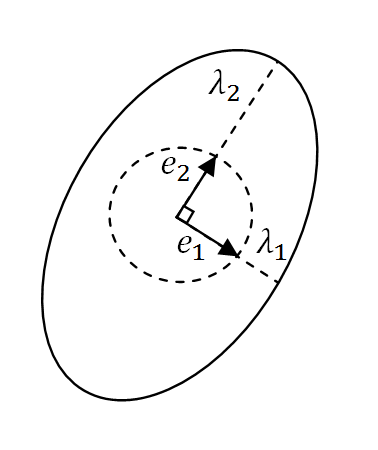
\includegraphics[scale=0.5]{l1_2}\end{center}
\textbf{Пример 3.}\\
Найти $A^+$.\\
\[A = \begin{pmatrix}
1 & 0 & 0 \\         
0 & 1 & 0 \\
0 & 0 & 1 \\
1 & 1 & 1 \\
\end{pmatrix}\]\\
\\
Найдем матрицу Грама.\\
\[A^*A = \begin{pmatrix}
1 & 0 & 0 & 1 \\         
0 & 1 & 0 & 1\\
0 & 0 & 1 & 1\\
\end{pmatrix} \cdot \begin{pmatrix}
1 & 0 & 0 \\         
0 & 1 & 0 \\
0 & 0 & 1 \\
1 & 1 & 1 \\
\end{pmatrix} = \begin{pmatrix}
2 & 1 & 1 \\         
1 & 2 & 1 \\
1 & 1 & 2 \\
\end{pmatrix}\]\\
\[(A^*A)^{-1} = \begin{pmatrix}[r]
\cfrac{3}{4} & -\cfrac{1}{4} & -\cfrac{1}{4} \\         
-\cfrac{1}{4} & \cfrac{3}{4} & -\cfrac{1}{4} \\
-\cfrac{1}{4} & -\cfrac{1}{4} & \cfrac{3}{4} \\
\end{pmatrix}\]
\begin{center}$det (A^*A)=2\cdot 3-(2-1)+(1-2)=6-1-1=4$\end{center}
\[A^+ = \begin{pmatrix}[r]
\cfrac{3}{4} & -\cfrac{1}{4} & -\cfrac{1}{4} \\         
-\cfrac{1}{4} & \cfrac{3}{4} & -\cfrac{1}{4} \\
-\cfrac{1}{4} & -\cfrac{1}{4} & \cfrac{3}{4} \\
\end{pmatrix} \cdot \begin{pmatrix}
1 & 0 & 0 & 1 \\         
0 & 1 & 0 & 1\\
0 & 0 & 1 & 1\\
\end{pmatrix} = \frac{1}{4} \cdot \begin{pmatrix}[r]
3 & -1 & -1 & 1 \\         
-1 & 3 & - 1 & 1 \\
-1 & -1 & 3 & 1 \\
\end{pmatrix}\]\\
\\
\textbf{Теорема.}
Если $B$ --- матрица полного строчного ранга (строки линейно независимы), то есть $rkB=m$, то $B^+=B^*(BB^*)^{-1}$.\\ \\
\textbf{Утверждение.}
Любую прямоугольную матрицу $A_{m \times n}$ можно представить в виде 
$A_{m \times n}=B_{m \times r}C_{r \times n}, r=rkA$, где $B$ --- матрица полного столбцового ранга, а $C$ --- матрица полного строчного ранга.\\
Такое разложение называется \textbf{скелетным разложением} (разложением полного ранга).\\ \\
\textbf{Пример 4.}\\
Найти скелетное разложение.\\
\[A = \begin{pmatrix}[r]
2 & -1 & 0 \\         
-1 & 1 & 1 \\
0 & 1 & 2 \\
\end{pmatrix}\]
Приведем к ступенчатому виду.\\
\[\begin{pmatrix}[r]
2 & -1 & 0 \\         
-1 & 1 & 1 \\
0 & 1 & 2 \\
\end{pmatrix} \approx \begin{pmatrix}[r]
1 & 0 & 1 \\         
-1 & 1 & 1\\
0 & 1 & 2\\
\end{pmatrix} \approx \begin{pmatrix}
1 & 0 & 1 \\         
0 & 1 & 2 \\
0 & 1 & 2 \\
\end{pmatrix} \approx \begin{pmatrix}
1 & 0 & 1 \\         
0 & 1 & 2 \\
0 & 0 & 0 \\
\end{pmatrix}\]\\
$rkA=2$\\
Надо найти такие $B$ и $C$, что $A_{3 \times 3}=B_{3 \times 2}C_{2 \times 3}$.
\[B = \begin{pmatrix}[r]
2 & -1 \\         
-1 & 1 \\
0 & 1 \\
\end{pmatrix}, ~ C = \begin{pmatrix}
1 & 0 & 1 \\         
0 & 1 & 2 \\
\end{pmatrix}\]
Здесь $B$ --- столбцы исходной матрицы, $C$ --- канонический вид.\\ \\
\textbf{Утверждение.}
Для скелетного разложения $A^+=(BC)^+=C^+B^+$, где 
$B^+=(B^*B)^{-1}B^*$, так как столбцевого ранга, а
$C^+=C^*(CC^*)^{-1}$, так как строчного ранга.\\ \\
(продолжение решения)
\[B^* = \begin{pmatrix}[r]
2 & -1 & 0 \\         
-1 & 1 & 1 \\
\end{pmatrix}, B^*B = \begin{pmatrix}[r]
2 & -1 & 0 \\         
-1 & 1 & 1 \\
\end{pmatrix} \cdot \begin{pmatrix}[r]
2 & -1 \\         
-1 & 1 \\
0 & 1 \\
\end{pmatrix} = \begin{pmatrix}[r]
5 & -3 \\         
-3 & 3 \\
\end{pmatrix}\]\\
\[(BB^*)^{-1} = \frac{1}{6} \cdot \begin{pmatrix}
3 & 3 \\         
3 & 5 \\
\end{pmatrix}^T = \frac{1}{6} \cdot \begin{pmatrix}
3 & 3 \\         
3 & 5 \\
\end{pmatrix}\]\\
\[B^+ = \frac{1}{6} \cdot \begin{pmatrix}
3 & 3 \\         
3 & 5 \\
\end{pmatrix} \cdot \begin{pmatrix}[r]
2 & -1 & 0 \\         
-1 & 1 & 1 \\
\end{pmatrix} = \frac{1}{6} \cdot \begin{pmatrix}
3 & 0 & 3 \\         
1 & 2 & 5 \\
\end{pmatrix}\]\\
\[C^* = \begin{pmatrix}
1 & 0 \\         
0 & 1 \\
1 & 2 \\
\end{pmatrix}, CC^* = \begin{pmatrix}
1 & 0 & 1 \\         
0 & 1 & 2 \\
\end{pmatrix} \cdot \begin{pmatrix}
1 & 0 \\         
0 & 1 \\
1 & 2 \\
\end{pmatrix} = \begin{pmatrix}
2 & 2 \\         
2 & 5 \\
\end{pmatrix}\]\\
\[(CC^*)^{-1} = \frac{1}{6} \cdot \begin{pmatrix}[r]
5 & -2 \\         
-2 & 2 \\
\end{pmatrix}^T = \frac{1}{6} \cdot \begin{pmatrix}[r]
5 & -2 \\         
-2 & 2 \\
\end{pmatrix}\]\\
\[C^+ = \begin{pmatrix}
1 & 0 \\         
0 & 1 \\
1 & 2 \\
\end{pmatrix} \cdot \frac{1}{6} \cdot \begin{pmatrix}[r]
5 & -2 \\         
-2 & 2 \\
\end{pmatrix} = \frac{1}{6} \cdot \begin{pmatrix}[r]
5 & -2 \\         
-2 & 2 \\
1 & 2 \\
\end{pmatrix}\]\\
\[A^+ = C^+B^+ = \frac{1}{6} \cdot \begin{pmatrix}[r]
5 & -2 \\         
-2 & 2 \\
1 & 2 \\
\end{pmatrix} \cdot \frac{1}{6} \cdot \begin{pmatrix}
3 & 0 & 3 \\         
1 & 2 & 5 \\
\end{pmatrix} = \frac{1}{36} \cdot \begin{pmatrix}[r]
13 & -4 & 5 \\         
-4 & 4 & 4 \\
5 & 4 & 13 \\
\end{pmatrix}\]\\
\\
\textbf{Домашнее задание 1}\begin{enumerate}
\item Вычислите \[\begin{pmatrix} 1&0\end{pmatrix}^+\]
\item Вычислите \[\begin{pmatrix} ~0~\\~1~\\~2~\\~3~\end{pmatrix}^+\]
\item Вычислите \[\begin{pmatrix} 3&2&1&0 \end{pmatrix}^+\]
\item Вычислите \[\begin{pmatrix}[r] 1&0~\\-1 & 0~\\-1 & 0~\\ 2&1~\end{pmatrix}^+\]
\item Вычислите  \[\begin{pmatrix}[r] 1&2&3\\0 & -1 & -2\end{pmatrix}^+\]
\item Пусть $A $ --- матрица размера $m\times n$
с рангом $r$ и пусть
$$
 K = \left[ \begin{array}{c} G \\ \hline  0\end{array} \right]
$$
имеет канонический вид,
где $G$ верхняя $r\times n$ подматрица без нулевых строк и
$0$ означает нулевую подматрицу. Пусть $i_1, \dots ,i_r$ значения столбцов, где находятся ведущие коэффициенты ступенчатого разложения, и пусть $F$ подматрица $A$ получена из столбцов $i_1,
\dots , i_r$.  Докажите, что
$$
A = FG
$$
 и что это разложение полного ранга (скелетное разложение) $A$.
\item Найти разложение полного ранга (скелетное разложение)
\[\begin{pmatrix}[r] ~1&1&1~\\~2 & 2 & 2~\\~3 & 3 & 3~\\ ~1&2&3~\end{pmatrix}\]
\item Вычислите  \[\begin{pmatrix}[r] ~1&0&0~\\~1 & 1 & 1~\\~0 & 1 & 1~\end{pmatrix}^+\]
\item Пусть $E_{ij}$ матрица размера $n\times n$, такая что ее элементы в $i$-ой строке и $j$-ом столбце единицы, а все остальные элементы нули. Найти разложение полного ранга и псевдообратную матрицу.
\item Докажите:\begin{enumerate}
\item $Im(AA^+) = Im(AA^*) = Im A$;
\item $Ker (AA^+) = Ker (AA^*) = Ker A^*$;
\item $Im A^+ = Im A^*$;
\end{enumerate}
\end{enumerate}
\section *{Лекция 2}
\noindent \textbf{Пример 1.}\\
Найти псевдообратную матрицу.\\
\[A = CB = \begin{pmatrix}
1 & 1 \\         
2 & 2 \\
3 & 3 \\
1 & 2 \\
\end{pmatrix} \cdot \begin{pmatrix}[r]
1 & 0 & -1 \\         
0 & 1 & 2 \\
\end{pmatrix}\]
\begin{center}
$A^+=B^+C^+$\\
$B^+=B^*(BB^*)^{-1}, ~C^+=(A^*A)^{-1}A^*$\\
\end{center}
\[BB^* = \begin{pmatrix}[r]
1 & 0 & -1 \\         
0 & 1 & 2 \\
\end{pmatrix} \cdot \begin{pmatrix}[r]
1 & 0 \\         
0 & 1 \\
-1 & 2 \\
\end{pmatrix} =  \begin{pmatrix}[r]
2 & -2 \\         
-2 & 5 \\
\end{pmatrix}\]\\
\[(BB^*)^{-1} = \frac{1}{6} \cdot \begin{pmatrix}
5 & 2 \\         
2 & 2 \\
\end{pmatrix}\]\\
\[B^+ = \frac{1}{6} \cdot \begin{pmatrix}[r]
1 & 0 \\         
0 & 1 \\
-1 & 2
\end{pmatrix} \cdot \begin{pmatrix}
5 & 2 \\         
2 & 2 \\
\end{pmatrix} = \frac{1}{6} \cdot \begin{pmatrix}[r]
5 & 2 \\         
2 & 2 \\
-1 & 2 \\
\end{pmatrix}\]\\
\[C^*C = \begin{pmatrix}
1 & 2 & 3 & 1 \\         
1 & 2 & 3 & 2 \\
\end{pmatrix} \cdot \begin{pmatrix}
1 & 1 \\         
2 & 2 \\
3 & 3 \\
1 & 2 \\
\end{pmatrix} =  \begin{pmatrix}
15 & 16 \\         
16 & 18 \\
\end{pmatrix}\]\\
\[(C^*C)^{-1} = \frac{1}{14} \cdot \begin{pmatrix}[r]
18 & -16 \\         
-16 & 15 \\
\end{pmatrix}\]\\
\[C^+ = \frac{1}{14} \cdot \begin{pmatrix}[r]
18 & -16 \\         
-16 & 15 \\
\end{pmatrix} \cdot \begin{pmatrix}
1 & 2 & 3 & 1 \\         
1 & 2 & 3 & 2 \\
\end{pmatrix} = \frac{1}{14} \cdot \begin{pmatrix}[r]
2 & 4 & 6 & -14 \\         
-1 & -2 & -3 & 14 \\
\end{pmatrix}\]\\
\[A^+ = B^+C^+ = \frac{1}{6} \cdot \frac{1}{14} \cdot \begin{pmatrix}[r]
5 & 2 \\         
2 & 2 \\
-1 & 2 \\
\end{pmatrix} \cdot \begin{pmatrix}[r]
2 & 4 & 6 & -14 \\         
-1 & -2 & -3 & 14 \\
\end{pmatrix} = \frac{1}{84} \cdot \begin{pmatrix}[r]
8 & 16 & 24 & -42 \\         
2 & 4 & 6 & 0 \\
-4 & -8 & -12 & 42 \\
\end{pmatrix}\]\\
\\
Если $A=FG$ --- скелетное разложение, то 
$A^+=G^+F^+=G^*(GG^*)^{-1}(F^*F)^{-1}F^*=XY$ и 
$X^*=X, Y^*=Y$, 
$rk(A^*A)=rkA$.\\
\\
\textbf{Утверждение.}
$X$ --- решение $AX=B$ тогда и только тогда, когда $X$ --- решение $A^*AX=A^*B$.\\
Если $N=A^*A$, то $N^*=N$ --- квадратная самосопряженная матрица.\\
\\
\textbf{Пример 2.}\begin{enumerate}
\item $Im(AA^*)\overset{?}{=}ImA$\\
Из доказательства леммы $rk(A^*A)=rkA$ --- ранги равны, значит и размерности равны.
\begin{center} $ImA=\{AX\} \supset \{AA^*Y\}=ImAA^*$\\
$dim(ImA)=dim(ImAA^*)$
\end{center}
\item $Im(AA^*)=ImA\overset{?}{=}Im(AA^+)$
\begin{center}
$ImA\supset Im(AA^+) \supset Im(AA^+A) \overset{1}{=} ImA$
\end{center}
\item $ImA^* \overset{?}{=} ImA^+$\\
$KerA^* \overset{?}{=} KerA^+$\\
Достаточно доказать одно из утверждений.
\begin{center}
$ImA^+ \supset Im(A^+A) \supset Im(A^+AA^+) = ImA^+$\\
$ImA^+=(ImA^+A) \overset{4}{=} Im(A^+A)^* = Im(A^*(A^+)^*) \subset ImA^*$\\
$rkA^+=rk(FG)^+=rk(G^+F^+)=rk(GF) \leqslant r = rkA$\\
$rkA=rk(A^+)^+ \leqslant rk A^+$
\end{center}
То есть получили, что $rkA^+=rkA=rkA^*$ --- ранги равны, а значит равны и размерности:
\begin{center}
$ImA^+=ImA^*$\\
$KerA^+=KerA^*$
\end{center}
\end{enumerate}
\textbf{Теорема.}
Пусть $A\bar x = \bar b$ --- система линейных уравнений, которая может не иметь решение, тогда $\bar u$ --- решение системы по \textbf{методу наименьших квадратов}, если для $\forall x$ длина вектора $A\bar x - \bar b$ не меньше, чем длина вектора $A\bar u - \bar b$, то есть если $f(x)=A\bar x - \bar b \in \mathbb{C}^n$, то $|f_1|^2+...+|f_n|^2$ минимально при $\bar x = \bar u$.\\
\\
\textbf{Теорема.}
Вектор $\bar u = A^+ \bar b$ является решением системы $A\bar x = \bar b$ по методу наименьших квадратов (мнк), причем среди всех этих решений вектор $\bar u$ имеет наименьшую длину. Решение по методу наименьших квадратов также называют псевдорешением.\\
\\
\textbf{Пример 3.}\\ 
Найти решение системы по методу наименьших квадратов.\\ \\
$
\left\{  
\begin{array}{ccl}  
    2x+y=1\\
    2x+y=3\\
\end{array}   
\right.  
$
\\ 
\\Перепишем в матричном виде:\\
\[\begin{pmatrix}
2 & 1 \\         
2 & 1 \\
\end{pmatrix} \cdot \begin{pmatrix}
x \\         
y \\
\end{pmatrix} = \begin{pmatrix}
1 \\         
3 \\
\end{pmatrix}\]\\
\[\begin{pmatrix}
x \\         
y \\
\end{pmatrix} = \begin{pmatrix}
2 & 1 \\         
2 & 1 \\
\end{pmatrix}^+\cdot \begin{pmatrix}
1 \\         
3 \\
\end{pmatrix} = \bigg( \begin{pmatrix}
1 \\         
1 \\
\end{pmatrix} \cdot \begin{pmatrix}
2 & 1 \\         
\end{pmatrix}\bigg)^+ \cdot \begin{pmatrix}
1 \\         
3 \\
\end{pmatrix} = \frac{1}{5} \cdot \begin{pmatrix}
2 \\         
1 \\
\end{pmatrix} \cdot \frac{1}{2} \cdot \begin{pmatrix}
1 & 1 \\         
\end{pmatrix} \cdot \begin{pmatrix}
1 \\
3 \\
\end{pmatrix} = \frac{1}{10} \cdot \begin{pmatrix}
2 \\
1 \\
\end{pmatrix} \cdot 4 = \begin{pmatrix}
0.8 \\
0.4 \\
\end{pmatrix}\]
\begin{center}
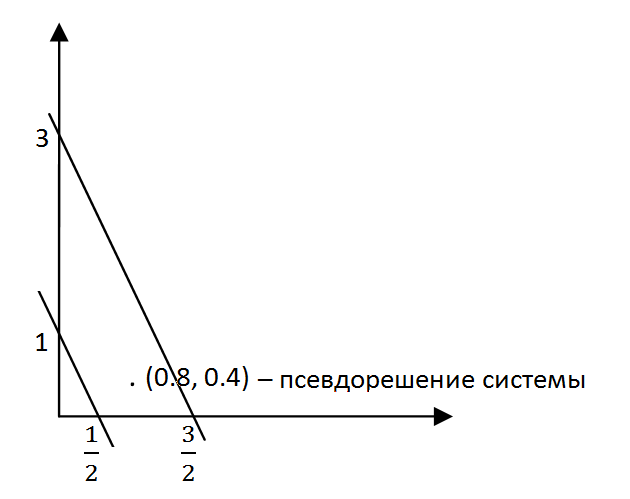
\includegraphics[scale=0.6]{l2_1.png}
\end{center}
\textbf{Сингулярное разложение (SVD).} \\
$A=Q \Sigma P^*$
$A: X \to Y$ --- отображение, где $X$ --- размерности $n$, а $Y$ --- размерности $m$.\\
\[\Sigma = \begin{pmatrix}
\sigma_1 & 0 & \cdots & \cdots & 0 \\
0 & \ddots & \cdots & \cdots & 0 \\
\vdots & \cdots & \sigma_r & \cdots & \vdots \\
\vdots & \cdots & \cdots & 0 & \vdots \\
0 & \cdots & \cdots & \cdots & 0 \\
\end{pmatrix}\]\\
$Q$ --- ортогональная матрица $m \times m$, 
$P$ --- ортогональная матрица $n \times n$, 
$\sigma_1 \geqslant ... \geqslant \sigma_r > 0$.\\ \\
Для $A^*A$ существует базис из собственных векторов $e_1,...,e_n$ (где она диагональна).\\
Она неотрицательно определена и существуют собственные векторы $A^*Ae_i=\sigma_i^2e_i$.\\ \\
$
\left\{  
\begin{array}{ccl}  
    f_1=\cfrac{Ae_1}{\sigma_1}\\
    \cdots\\
    f_r=\cfrac{Ae_r}{\sigma_r}\\  
\end{array}   
\right.  
$
\\ \\
$
Ae_i = \left\{\begin{array}{ll}  
    \sigma_if_i,& i \leqslant r\\
    0,& i > r\\
\end{array}   
\right.  
$
\\ \\
$
A^*f_i=\left\{\begin{array}{ll}  
    \sigma_ie_i,& i \leqslant r\\
    0,& i > r\\
\end{array}   
\right.  
$
\\ \\
В матрице $Q$ по столбцам стоят векторы $f_1,...,f_r$ (уже получены), $f_{r+1},...,f_m$ (из ортогонализации Грама-Шмидта) в базисе $Y$.\\
$P$ --- столбцы координат $e_1,...,e_n$ в базисе $X$.\\
\\
\textbf{Пример 4.}\\
Найти SVD.\\
\[\tilde{A} = \begin{pmatrix}
1 & 0 & 0 & 1 \\         
0 & 1 & 0 & 1 \\
0 & 0 & 1 & 1 \\
\end{pmatrix}\]
\\
\[\tilde{A}^*\tilde{A} = \begin{pmatrix}
1 & 0 & 0 \\         
0 & 1 & 0 \\
0 & 0 & 1 \\
1 & 1 & 1 \\
\end{pmatrix} \cdot \begin{pmatrix}
1 & 0 & 0 & 1\\         
0 & 1 & 0 & 1\\
0 & 0 & 1 & 1\\
\end{pmatrix} = \begin{pmatrix}
1 & 0 & 0 & 1\\         
0 & 1 & 0 & 1\\
0 & 0 & 1 & 1\\
1 & 1 & 1 & 3\\
\end{pmatrix}\]\\
Найдем собственные значения и векторы $\tilde{A}^*\title{A}$.
\begin{center}
$\lambda_1=0$\\
$\lambda_2=1$\\
$\lambda_3=1$\\
$\lambda_4=4$\\
\end{center}
Сингулярные числа надо расположить по убыванию.
\begin{center}
$\sigma_1=\sqrt{4}=2$\\
$\sigma_2=1$\\
$\sigma_3=1$\\
$\sigma>0$\\
\end{center}
\[\Sigma_{3 \times 4} = \begin{pmatrix}
2 & 0 & 0 & 0\\         
0 & 1 & 0 & 0\\
0 & 0 & 1 & 0\\
\end{pmatrix}\]
\\
Найдем собственные векторы.
\begin{enumerate}
\item $\lambda = 4$\\
\begin{center}
$(\tilde{A}^*\tilde{A}-\lambda_iE)x=0$\\
\[\begin{pmatrix}[r]
-3 & 0 & 0 & 1\\         
0 & -3 & 0 & 1\\
0 & 0 & -3 & 1\\
1 & 1 & 1 & -1\\
\end{pmatrix}\cdot x = 0\]
\\
$x_1=\cfrac{1}{3}x_4$, 
$x_2=\cfrac{1}{3}x_4$, 
$x_3=\cfrac{1}{3}x_4$
\end{center}
Получим собственный вектор: \[\begin{pmatrix}
1\\         
1\\
1\\
3\\
\end{pmatrix} \cdot c, c\neq 0\]
\\
\[e_1 = \frac{1}{2\sqrt{3}} \cdot \begin{pmatrix}
1\\         
1\\
1\\
3\\
\end{pmatrix}\]
\item $\lambda=1$\\
\[\begin{pmatrix}
0 & 0 & 0 & 1\\         
0 & 0 & 0 & 1\\
0 & 0 & 0 & 1\\
1 & 1 & 1 & 2\\
\end{pmatrix} \approx \begin{pmatrix}
0 & 0 & 0 & 1\\         
1 & 1 & 1 & 0\\
\end{pmatrix}\]
\\
Получим собственные векторы: \[\begin{pmatrix}[r]
-1~\\         
0~\\
1~\\
0~\\
\end{pmatrix} \cdot c_1 + \begin{pmatrix}[r]
-1~\\         
1~\\
0~\\
0~\\
\end{pmatrix}\cdot c_2,~ c_1^2+c_2^2>0\]
\\
\[e_2 = \begin{pmatrix}[r]
-\cfrac{1}{\sqrt{2}}~\\         
\cfrac{1}{\sqrt{2}}~\\
0~\\
0~\\
\end{pmatrix}, e_3 = \cfrac{1}{\sqrt{6}} \cdot \begin{pmatrix}[r]
1~\\         
1~\\
-2~\\
0~\\
\end{pmatrix}, e_4 = \cfrac{1}{2} \cdot \begin{pmatrix}[r]
1~\\         
1~\\
1~\\
-1~\\
\end{pmatrix}\]
\end{enumerate}
\begin{center} $P=(e_1, e_2, e_3, e_4)$ \end{center}
\[f_1=\frac{\tilde{A}e_1}{\sigma_1}=\frac{1}{2\sqrt{3}} \cdot \begin{pmatrix}
4\\         
4\\
4\\
\end{pmatrix} \cdot \frac{1}{2} = \begin{pmatrix}
\cfrac{1}{\sqrt{3}}\\         
\cfrac{1}{\sqrt{3}}\\
\cfrac{1}{\sqrt{3}}\\
\end{pmatrix} = \frac{1}{\sqrt{3}} \cdot \begin{pmatrix}
1\\         
1\\
1\\
\end{pmatrix}\]
\\
\[f_2=\frac{\tilde{A}e_2}{\sigma_2}=\frac{1}{\sqrt{2}} \cdot \begin{pmatrix}[r]
-1~\\         
1~\\
0~\\
\end{pmatrix}\]
\\
\[f_3=\frac{\tilde{A}e_3}{\sigma_3}=\frac{1}{\sqrt{6}} \cdot \begin{pmatrix}[r]
1~\\         
1~\\
-2~\\
\end{pmatrix}\]
\begin{center} $Q=(f_1, f_2, f_3)$ \end{center}
\[Q = \begin{pmatrix}[r]
\cfrac{1}{\sqrt{3}} & -\cfrac{1}{\sqrt{2}} & \cfrac{1}{\sqrt{6}}\\ \cfrac{1}{\sqrt{3}} & \cfrac{1}{\sqrt{2}} & \cfrac{1}{\sqrt{6}}\\ \cfrac{1}{\sqrt{3}} & 0 & -\cfrac{2}{\sqrt{6}}\\ 
\end{pmatrix}\]
\\
\[\tilde{A} = Q \Sigma P^* = \begin{pmatrix}[r]
\cfrac{1}{\sqrt{3}} & -\cfrac{1}{\sqrt{2}} & \cfrac{1}{\sqrt{6}}\\ \cfrac{1}{\sqrt{3}} & \cfrac{1}{\sqrt{2}} & \cfrac{1}{\sqrt{6}}\\ \cfrac{1}{\sqrt{3}} & 0 & -\cfrac{2}{\sqrt{6}}\\ 
\end{pmatrix} \cdot \begin{pmatrix}
2 & 0 & 0 & 0\\         
0 & 1 & 0 & 0\\
0 & 0 & 1 & 0\\
\end{pmatrix} \cdot \begin{pmatrix}[r]
\cfrac{1}{2\sqrt{3}} & -\cfrac{1}{\sqrt{2}} & \cfrac{1}{\sqrt{6}} & \cfrac{1}{2}\\ 
\cfrac{1}{2\sqrt{3}} & \cfrac{1}{\sqrt{2}} & \cfrac{1}{\sqrt{6}} & \cfrac{1}{2}\\ 
\cfrac{1}{2\sqrt{3}} & 0 & -\cfrac{2}{\sqrt{6}} & \cfrac{1}{2}\\
\cfrac{3}{2\sqrt{3}} & 0 & 0 & -\cfrac{1}{2}\\
\end{pmatrix}^*=\]\\ \[= \begin{pmatrix}[r]
\cfrac{2}{\sqrt{3}} & -\cfrac{1}{\sqrt{2}} & \cfrac{1}{\sqrt{6}} & 0\\ 
\cfrac{2}{\sqrt{3}} & \cfrac{1}{\sqrt{2}} & \cfrac{1}{\sqrt{6}} & 0\\ 
\cfrac{2}{\sqrt{3}} & 0 & -\cfrac{2}{\sqrt{6}} & 0\\
\end{pmatrix} \cdot \begin{pmatrix}[r]
\cfrac{1}{2\sqrt{3}} & \cfrac{1}{2\sqrt{3}} & \cfrac{1}{2\sqrt{3}} & \cfrac{3}{2\sqrt{3}}\\ 
-\cfrac{1}{\sqrt{2}} & \cfrac{1}{\sqrt{2}} & 0 & 0\\ 
\cfrac{1}{\sqrt{6}} & \cfrac{1}{\sqrt{6}} & -\cfrac{2}{\sqrt{6}} & 0\\
\cfrac{1}{2} & \cfrac{1}{2} & \cfrac{1}{2} & -\cfrac{1}{2}\\
\end{pmatrix} = \begin{pmatrix}
1 & 0 & 0 & 1\\         
0 & 1 & 0 & 1\\
0 & 0 & 1 & 1\\
\end{pmatrix}\]
\\
\textbf{Утверждение.}
Если $B=AU$, где $U^*=U^{-1}$ унитарная, то $B^+=U^+A^+=U^*A^+$.\\ \\
\textbf{Следствие.}
Если $A=Q\Sigma P^*$, то \[A^+=P\Sigma^+Q^*=P \cdot \begin{pmatrix}
\sigma_1^{-1} & \cdots & 0 \\         
\vdots & \sigma_2^{-1} & \vdots \\
0 & \cdots & \ddots \\
\end{pmatrix} \cdot Q^*\]
\textbf{Линейная регрессия.}\\
\textbf{Модель 1:}\begin{center}
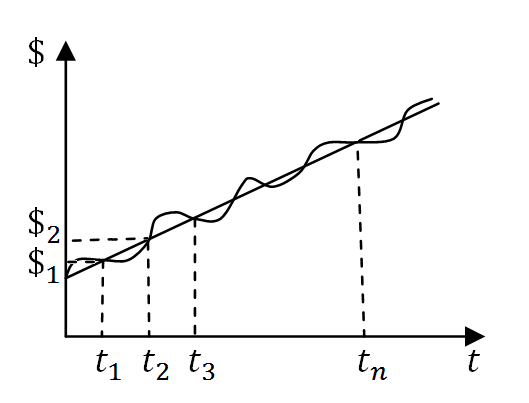
\includegraphics[scale=0.7]{l2_2.png}\end{center}
$\$ = kt+b$\\ \\
$
\left\{  
\begin{array}{ccl}  
    \$_1=kt_1+b\\
    \$_2=kt_2+b\\
    \cdots\\
\end{array}   
\right.  
$\\ \\
Надо найти $k$ и $b$.\\
В матричном виде $A\bar X=\bar S$, где\\
\[X = \begin{bmatrix}
k\\         
b\\
\end{bmatrix}, A = \begin{pmatrix}
t_1 & 1\\         
t_2 & 1\\
\vdots & \vdots\\
t_n & 1\\
\end{pmatrix}, S = \begin{pmatrix}
\$_1\\         
\vdots\\
\$_n\\
\end{pmatrix}\]\\
\[\begin{bmatrix}
k\\         
b\\
\end{bmatrix} = \bar X = A^+\bar S\]\\
\textbf{Модель 2:}\\
Если $x(t)$ --- цена на нефть, то $\$(t)x(t)=k_1t+b_1$.\\
\\
\textbf{Домашнее задание 2}
\begin{enumerate}
\item
Доказать утверждение о псевдообратной от произведения матриц.
Если $B=AU$, где $U^*=U^{-1}$ --- унитарная матрица, а $A$ --- произвольная матрица порядка $n$, то $$B^+=U^+A^+=U^*A^+$$ 
\item
С помощью линейной регрессии и псевдообратной матрицы сделать прогноз цены нефти $Br$ в долларах, рублях. Сравнить результаты, полученные с помощью модели 1 и модели 2.
\item
Найти SVD для матрицы\\
\[A=\begin{pmatrix}[r]
4 & -3i\\
-3i & 4\\
\end{pmatrix}\]
\item
Найти SVD для матрицы\\
\[A=\begin{pmatrix}[r]
6 & 3 & 0\\
6 & 3 & 0\\
2 & 5 & 4\\
-2 & -5 & -4\\
\end{pmatrix}\]
\item
Найти псевдообратную матрицу, используя SVD:\\
\[A=\begin{pmatrix}[r]
18 & 18 & 9\\
4 & -2 & -4\\
8 & -4 & -8\\
8 & -4 & -8\\
\end{pmatrix}\]
\end{enumerate}
~\\
\section *{Лекция 3}
\noindent \textbf{Полиномиальная интерполяция.}\\
\textbf{Дано:} \\$f(x)$ --- неизвестный многочлен степени $\leq$ $n$\\
$f(x) = a_{0}+a_1x+...+a_nx^n$ \\
Известны значения $f(x)$ в точках $x_0, ..., x_n$ (всего $n+1$ значений)\\ 
$
\left\{  
\begin{array}{ccl}  
    y_0=f(x_0)\\
   \cdots\\
   y_n=f(x_n)\\  
\end{array}   
\right.  
$
\\
\\ \textbf{Найти:} $f(x)$
\\ \textbf{Ответ:} многочлен Лагранжа \\
\begin{equation*}
 \begin{cases}
   a_0+a_1x_0+...+a_nx_0^n = y_0\\
   \cdots\\
   a_0+a_1x_n+...+a_nx_n^n = y_n
 \end{cases}
\end{equation*}

\[\begin{pmatrix}
1 & x_0 & ... & x_0^n \\
\hdotsfor[1]{4} \\
1 & x_n & ... & x_n^n
\end{pmatrix} \cdot \begin{pmatrix}
a_0 \\
\vdots\\
a_n
\end{pmatrix} = \begin{pmatrix}
y_0 \\
\vdots\\
y_n
\end{pmatrix}\]
Матрица Вандермонда: $V(x_0,...,x_n)=V$ 
\begin{center}$V \bar a = \bar y$, $\bar a=V^{-1} \bar y$\end{center}
Определитель Вандермонда: $v(x_0,...,x_n) = det V(x_0,...,x_n) = (x_1-x_0)(x_2-x_0)...(x_n--x_0)(x_2-x_1)...(x_n-x_1)...(x_n-x_{n-1}) = \prod\limits_{0 \leq i < j \leq n} (x_j-x_i)$ 
\[ V = \begin{vmatrix}
1 & x_0 & ... & x_0^n \\
\hdotsfor[1]{4} \\
1 & x_n & ... & x_n^n
\end{vmatrix} = \begin{vmatrix}
1 & x_0 & ... & x_0^n \\
0 & x_1-x_0 & ... & x_1^n-x_0^n \\
\hdotsfor[2]{4} 
\end{vmatrix}\]
\begin{center}
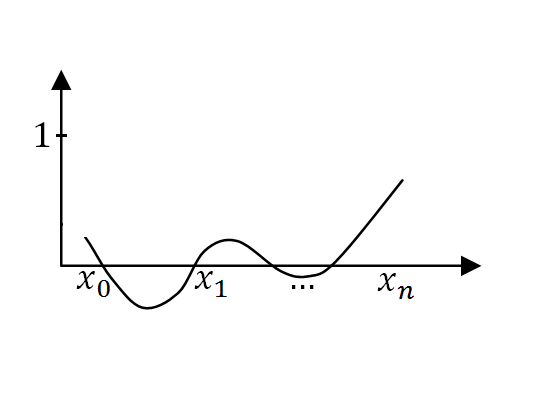
\includegraphics[scale=0.5]{l3_1.png}
\end{center}
Многочлен Лагранжа: \begin{center}$f(x)=L(x) = \sum\limits_{i=0}^{n} y_i \cdot \cfrac{\prod\limits_i (x-x_j)}{\prod\limits_j (x_i-x_j)} = \cfrac{\sum\limits_{i=0}^n y_i v(x_0,..., \underset{i}{x},..., x_n)}{v(x_0,..., x_n)}.$\end{center}
\noindent \textbf{Пример 1.}\\
Дано:\\
$x_0 = -1$, $x_1 = 0$, $x_2 = 1$\\
$y_0 = -2$, $y_1 = -1$, $y_2 = 2$\\
Провести параболу через три точки. Найти $f(x) = L(x) = a_0+a_1x+a_2x^2$.\\
\begin{center} $f(x) = \cfrac{-2(0-x)(1-x)+(-1)(x+1)(1+1)(1-x)+2(0+1)(x+1)(x-0)}{(0+1)(1+1)(1-0)} =$\\~\\$= x^2+2x-1$ \end{center}
\begin{center}
$f(x) = (x-1)g(x) \Leftrightarrow f(1) = 0$\\
$f(x) = (x-1)^2g(x) \Leftrightarrow$ 
$  
\left\{  
\begin{array}{lcl}  
    f(1) = 0 \\  
    f'(1) = 0 \\  
\end{array}   
\right.  
$
\\
$f'(x) = 2(x-1)g(x)+(x-1)^2g'(x)$
\end{center}
\noindent \textbf{Лемма.}
\begin{center}
$f(x) = (x-x_1)^kg(x) \Leftrightarrow$ 
$  
\left\{  
\begin{array}{lcl}  
    f(x_1) = 0 \\  
    f'(x_1) = 0 \\
    \cdots\\
    f^{(k-1)}(x_1) = 0\\
\end{array}   
\right.  
$
\end{center}
\noindent \textbf{Интерполяция с кратными узлами.}\\
\textbf{Задача (кратко):}
Восстановить многочлен $f(x)$ по значениям в $m$ точках кратностей $k_1,..., k_m$.\\
\textbf{Формулировка:}
Найти многочлен $f(x)$ степени $\leq$ $n-1$ такой, что для некоторых различных узлов $x_1,...,x_m$ и некоторых натуральных $k_1,...,k_m$ (кратностей) верно\\
$  
\left\{  
\begin{array}{lcl}  
    f(x_1) = y_1, f'(x_1) = y_1^{(1)},...,f^{(k_1-1)}(x_1) = y_1^{(k_1-1)} \\  
    ...\\
    f(x_m) = y_m, f'(x_m) = y_m^{(1)},...,f^{(k_m-1)}(x_m) = y_m^{(k_m-1)} \\
\end{array}   
\right.  
$
\\ \\
Количество условий равно количеству неизвестных $k_1+...+k_m = n$.\\
\textbf{Ответ:} Многочлен Эрмита (или Лагранжа-Сильвестра).\\
\\
\noindent \textbf{Утверждение.}
Такой многочлен существует и он единственный при $k_1+...+k_m = n$.\\
Примечание: Если $k_1 = ... = k_m = 1$, то $m = n$ и $f(x)$ - многочлен Лагранжа (то есть предыдущий случай).\\
$\blacktriangleright$
Пусть существует два таких многочлена $f(x)$ и $g(x)$, то для $p(x) = f(x)-h(x)$
\begin{center}
$p^{(t)}(x_i) = 0, i=1,...,m, t\leq k_i$\\
$p(x) = C(x-x_1)^{k_1}...(x-x_k)^{k_k} = C$ (многочлен степени $n+1$)\\
$\Rightarrow C = 0, p(x) = 0$
\end{center}
Значит, если $f(x)$ существует, то он единственный.\\
Если $f(x) = a_0+a_1x+...+a_{n-1}x^{n-1}$, то \\
\[A \begin{pmatrix}[l]
~a_0 \\
~a_1 \\
~\vdots\\
~a_{n-1}
\end{pmatrix} = \begin{pmatrix}[l]
~y_0 \\
~y_2^{(1)}\\
~\vdots\\
~y_m^{(k_m-1)}
\end{pmatrix}\]\\
То есть, доказали, что система для любого $\bar y$ имеет не больше одного решения $\bar a$.\begin{center}
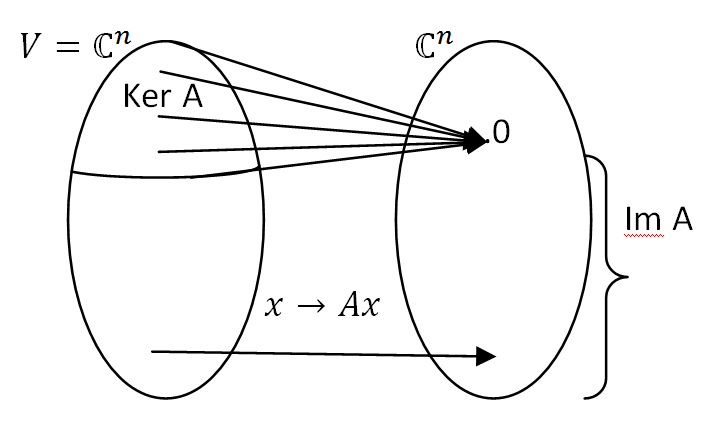
\includegraphics[scale=0.4]{l3_2.png}\end{center}
$Im A = \{ A \bar x | x\in \mathbb{C}^n \} $, 
$Ker A = \{\bar a | A \bar a = \bar 0 \} = \{\bar 0 \} $, так как у системы $A \bar a = \bar 0$ не больше одного решения.\\
Так как $A$ $n \times n$, то 
$dim(Im A) = rk A$, $dim(Ker A) = n-rk A$.\\ 
$Ker~ 0 \Leftrightarrow dim(Ker A) = 0$, то есть $rk A = n$ ($A$ невырожденная). \\
Матрица $A$ невырожденная $\Leftrightarrow$ $rk A = n \Leftrightarrow Im A = \mathbb{C}^n \Leftrightarrow Ker A = 0$, значит, $\bar a = A^{-1}\bar y$, всегда существует решение. $\blacksquare$\\
\\
\noindent \textbf{Сплайны.}\\
\noindent \textbf{1. Квадратичный.}\\
Надо установить функцию $f(x)$.\\
Аппроксимация: соседние точки надо соединить прямыми (не плавно). Но мы хотим гладко, значит на каждом отрезке надо задать свою функцию.\begin{center} 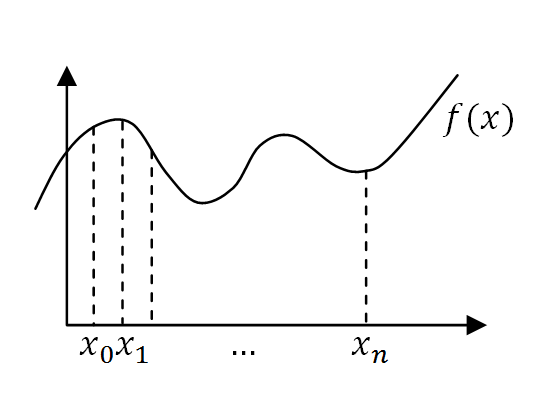
\includegraphics[scale=0.6]{l3_3.png}\\
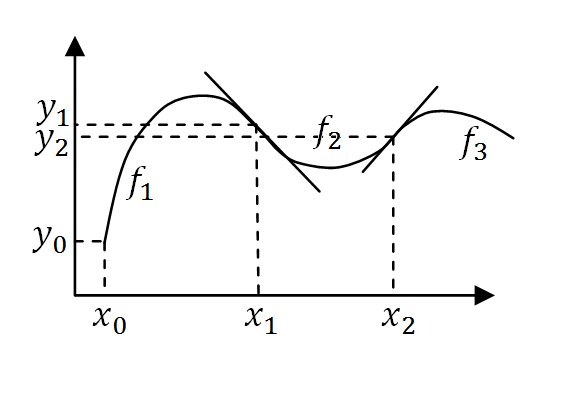
\includegraphics[scale=0.6]{l3_4.png}\end{center}
$  
\left\{  
\begin{array}{lcl}  
    f_1'(x_0) = d_0 \\  
    f_1(x_0) = y_0\\
    f_1(x_1) = y_1\\
\end{array}   
\right.  
$
\\ \\
$  
\left\{  
\begin{array}{lcl}  
    f_1'(x_1) = f_2'(x_1) \\  
    f_2(x_1) = y_1\\
    f_2(x_2) = y_2\\
\end{array}   
\right.  
$\\ \\
........... и т.д.\\
\\
\noindent \textbf{2. Кубический.}\\
$f_i(x)$ - кубическая парабола.\begin{center}
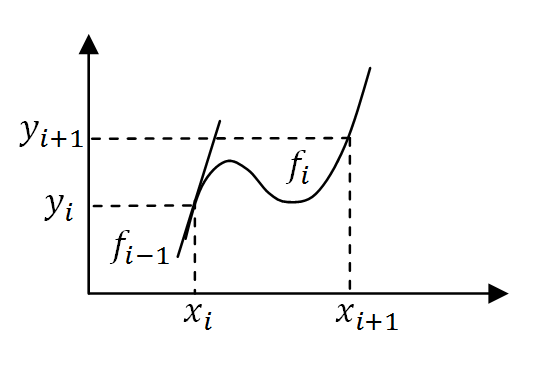
\includegraphics[scale=0.6]{l3_5.png}\end{center}
$  
\left\{  
\begin{array}{lcl}  
    f_i(x_i) = y_i \\  
    f_i(x_{i+1}) = y_{i+1}\\
    f_i'(x_i) = f_{i-1}'(x_i)\\
    f_i''(x_i) = f_{i-1}''(x_i)\\
\end{array}   
\right.  
$
\begin{center}
$f_i(x) = a_0^i+a_1^ix+a_2^ix^2+a_3^ix^3 = a_i+b_i(x-x_i)+ \cfrac{c_i}{2}(x-x_i)^2+ \cfrac{d_i}{6}(x-x_i)^3$
\end{center}
\noindent \textbf{Пример 2.}
\begin{center}$f(x) = (x-1)(x-2)(x-3) = x^3-6x^2+11x-6$\end{center}
Аппроксимировать квадратичным сплайном с узлами $x_0=0, x_1=2, x_2=4$.\\ \\
$  
\left\{  
\begin{array}{lcl}
f(0)=(-1)\cdot (-2)\cdot (-3)=-6\\
f(2)=0\\
f(4)=6\\
\end{array}   
\right.  
$
\\ \\
$  
\left\{  
\begin{array}{lcl}
f_1 = a_0+a_1x+a_2x^2\\
f_1'(0) = a_1 = 11\\
f_1(0) = a_0 = -6\\
f_1(2) = -6+11\cdot 2+a_2\cdot 4 = 0 \Rightarrow a_2 = -4\\
\end{array}   
\right.  
$
\\ \\
Получим $f_1 = -6+11x-4x^2$. \\ \\
$  
\left\{  
\begin{array}{lcl}
f_1 = -6+11x-4x^2\\
f_2'(2) = f_1'(2) = -5\\
f_2(2) = 0\\
f_2(4) = 6\\
\end{array}   
\right.  
$
\\ ~\\
Подставим значения из предыдущих выражений.\\ \\
$
\left\{  
\begin{array}{lcl}
f_2 = b_0+b_1x+b_2x^2\\
b_0+2b_1+4b_2 = 0\\
b_1+4b_2 = -5\\
b_0+4b_1+16b_2 = 6\\
\end{array}   
\right.  
$
\\ \\
Получим $f_2 = 4x^2-21x+26$.\begin{center}
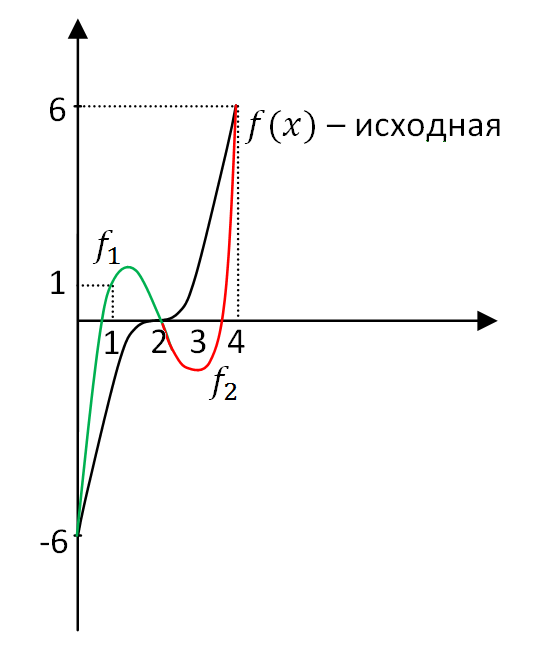
\includegraphics[scale=0.7]{l3_6.png}\end{center}
\noindent \textbf{Кривая Безье.}\\
Есть набор из $n$ точек, хотим построить прямую, хорошо вписываемую в оболочку.\\
Параметризация отрезка для 2 точек, степень полинома $n = 1$:
\begin{center}
$B(t) = (1-t)P_0+tP_1$\\
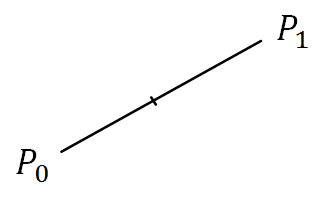
\includegraphics[scale=0.5]{l3_7.png}\end{center}
Параметризация отрезка для 3 точек, степень полинома $n = 2$.\\
Введем вспомогательные точки $M_1, M_2$ такие, что \begin{center}$M_1 = (1-t)P_0+tP_1$, $M_2 = (1-t)P_1+tP_2$\\
$B(t) = (1-t)M_1+tM_2 = (1-t)^2P_0+2t(1-t)P_1+t^2P_2$\\
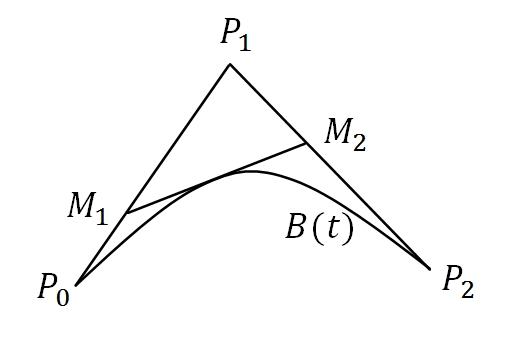
\includegraphics[scale=0.5]{l3_8.png}\end{center}
Параметризация отрезка для $n+1$ точек, степень полинома $n$.
\begin{center}$B(t) = \sum\limits_{k=0}^n C_n^k (1-t)^{n-k}t^kP_k$\end{center}
\noindent \textbf{Пример 3.}\\
Построить кубическую кривую Безье $B_3(t)$ для 4 точек, $t\in [0, 1]$.\begin{center}
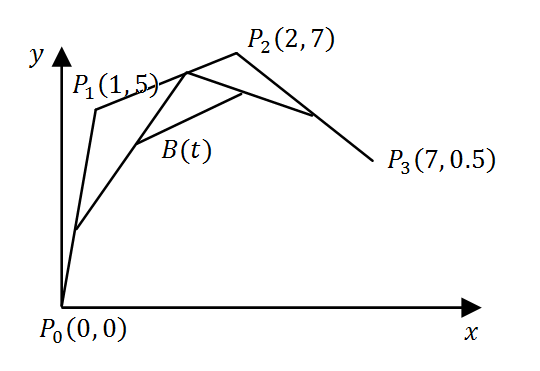
\includegraphics[scale=0.7]{l3_9.png}\end{center}
$x(t) = 1\cdot (1-t)^3\cdot t^0\cdot 0+3\cdot (1-t)^2\cdot t^1\cdot 1+3\cdot (1-t)^1\cdot t^2\cdot 2+(1-t)^0\cdot t^3\cdot 7 = 4t^3+3t$\\
$y(t) = 1\cdot (1-t)^3\cdot t\cdot 0+3\cdot (1-t)^2\cdot t\cdot 5+3\cdot (1-t)^1\cdot t^2\cdot 7+1\cdot (1-t)^0\cdot t^3\cdot \frac{1}{2} = - \frac{11}{2}t^3-9t^2+15t$\\ \\
\noindent \textbf{Домашнее задание 3}
\begin{enumerate}
\item Приблизить следующую функцию $y(x)$ многочленом второй степени по методу наименьших квадратов:\\
\begin{tabular}{|l|c|c|c|c|c|}
\hline
$x$ & -3 & -1 & 0 & 1 & 3 \\ \hline
$y$ & -4 & -0.8 & 1.6 & 2.3 & 1.5\\ \hline
\end{tabular}
\item
Доказать, что кривая Безье касается первого и последнего отрезка ломаной.
\item
Известно, что $f(x)$ --- многочлен третьей степени такой, что:\\ \\
$
\left\{
\begin{array}{lcl}
    f(1) = 2 \\
    f(-1) = -3 \\
    f(2) = 17\\
    f(-2) = -19\\
\end{array}
\right.
$\\
\\Найти $f(x)$.
\item
Найти $f(x)$ многочлен наименьшей степени, удовлетворяющий условиям:\\ \\
$
\left\{
\begin{array}{lcl}
    f(1) = -1 \\
    f'(1) = 5 \\
    f(0) = 0\\
    f'(0) = -1\\
\end{array}
\right.
$
\item
Приблизить $sin~x$ сплайном $S(x)$ степени два с узлами $\pi k$, $\pi k + \cfrac{\pi}{2}$, $k\in \mathbb{Z}$. Найти $S \Big(\cfrac{\pi}{4} \Big)$, $S \Big(\cfrac{\pi}{3} \Big)$.
\item На плоскости 100 точек, любые 4 из них лежат на параболе вида $y=ax^2+bx+c$. Доказать, что тогда все 100 точек будут лежать на одной и той же параболе.
\end{enumerate}
\section *{Лекция 4}
\noindent \textbf{Метрики, линейные пространства.}\\ \\
\textbf{Метрика} $\rho$ на множестве $M$ --- это такая функция $\rho (x, y) \geqslant 0$, что 
\begin{enumerate}
\item $\rho (x, y) = \rho (y, x)$
\item $\rho (x, y) > 0, x\neq y, \rho (x, x) = 0$ 
\item $\rho (x, y) + \rho (y, z) \geqslant \rho (x, z)$
\end{enumerate}
Дана карта с расстояниями между городами.\\
$M$ = \{ города \}\begin{center}
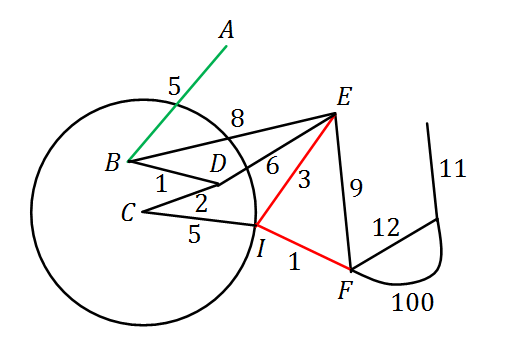
\includegraphics[scale=0.7]{l4_1.png}\end{center}
$\rho (A, B) = 5$\\
$\rho (E, F) = 4$ (минимальное расстояние из возможных)\\
\\
\textbf{Шар в метрическом пространстве.}\begin{center}
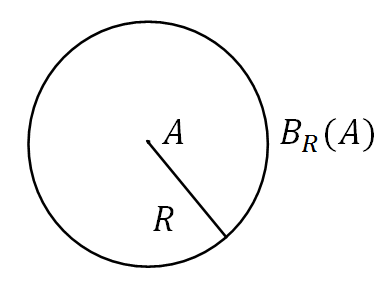
\includegraphics[scale=0.5]{l4_2.png}\end{center}
$B_R(A) = \{x | \rho(A, x) \leqslant R \}$ --- \textbf{шар} радиуса $R$ с центром в точке $A$.\\ 
$S_R(A) = \{x | \rho(A, x) = R \}$ --- \textbf{сфера} радиуса $R$ с центром в точке $A$.\\ 
\\
$B_5(C) = \{ C, B, D, I \}$ --- все точки, которые туда входят. \\
$S_5(C) = \{ I \}$ --- только те точки, которые лежат на окружности. \\
$B_{100}(C) = B_{50} (C) = M $ --- все множество. \\
\\
Метод наименьших квадратов --- приближение функции в смысле следующей метрики \begin{center} $M = \{f: X \rightarrow \mathbb{R} \}, X = \{ x_1, ..., x_n \}$\\ ~\\
$\rho (f, y) = |\bar y - \bar f| = \sqrt{\sum\limits_{i=1}^n(y(x_i)-f(x_i))^2}$ \\
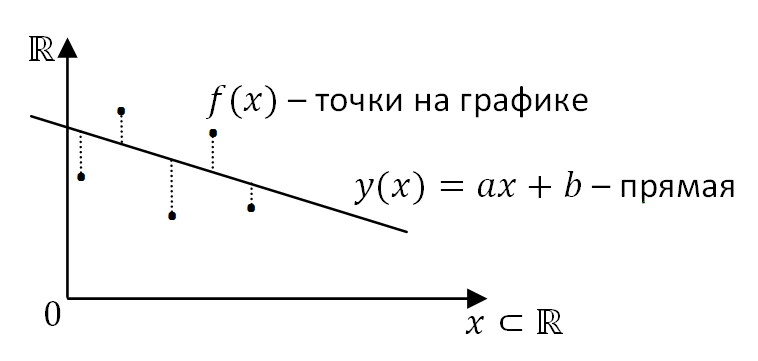
\includegraphics[scale=0.6]{l4_4.png}\end{center}
\noindent \textbf{Пример 1.}\\
Найти такое метрическое пространство $M$, что\\ \\
$  
\left\{  
\begin{array}{lcl}  
    B_5(x) \subset B_4(y) \\  
    B_5(x) \neq B_4(y)\\
\end{array}   
\right.  
$
, где $x, y$ - две точки. \\ \\То есть доказать, что существует $c\in B_4(y), c\notin B_5(x)$.\begin{center}
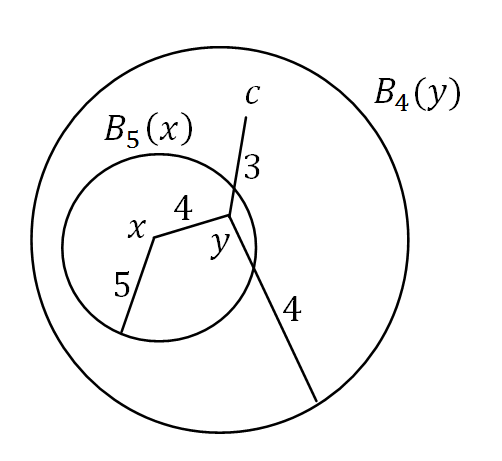
\includegraphics[scale=0.5]{l4_5.png}\\
$\rho (x, y) = \rho(y, x) = 4$\\
$\rho (y, c) = \rho(c, y) = 3$\\
$\rho (x, c) = \rho(c, x) = 7$\\
~\\
$B_5(x) = \{ x, y \}$\\
$B_4(y) = \{x, y, c \} $\end{center}
То есть $B_5(x) \subset B_4(y)$.\\
\\
Вспомним определение линейного пространства.\\
Если на непустом множестве заданы две бинарные операции "+" и "умножение на число", числа из поля $F$, $\forall ~a,~b,~c\in V$ то\begin{enumerate}
\item $a+(b+c) = (a+b)+c$
\item $\exists~0: a+0 = 0+a = a$
\item $\exists~ (-a): a+(-a) = 0$
\item $a+b = b+a$
\item $1\cdot x = x$
\item $ (\mu \lambda)x = \mu(\lambda x)$
\item $(a+b)\lambda = a\lambda + b\lambda$
\item $(\mu + \lambda)a = \mu a + \lambda a$
\end{enumerate}
$V$ --- \textbf{линейное пространство} (векторное пространство), если выполнены 8 предыдущих аксиом и \begin{enumerate}
\item $\forall \bar u, \bar v$: $\bar u + \bar v \in V$
\item $\forall$ числа $\alpha \in$ $\mathbb{R}$, $\mathbb{C}$ $\alpha \bar u \in V$\\ 
(или $\alpha \in F$ заданное поле, например, $F_2 = \{ 0, 1 \}$)\end{enumerate}
Линейное пространство $V$ --- \textbf{нормированное}, если на нем задана такая норма \\$\nu : V \to$ $\mathbb{R}$ $\geqslant 0$, что\begin{enumerate}
\item $\nu(\bar x) > 0$, $\bar x \neq \bar 0$, $\nu(\bar 0) = \bar 0$
\item $\nu(\alpha \bar x) = |\alpha|\nu(\bar x)$
\item $\nu(\bar x + \bar y) \leq \nu(\bar x) + \nu(\bar y)$ для $\forall x, y \in V, \forall \alpha$
\end{enumerate}
Из каждой нормы можно сделать метрику $\rho(\bar x, \bar y) = \nu(\bar y - \bar x)$.\\ \\
\textbf{Примеры норм:}\begin{enumerate}
\item Манхэттенская норма (норма таксиста)\\
(Можно ехать разными путями, но не по прямой)\begin{center}
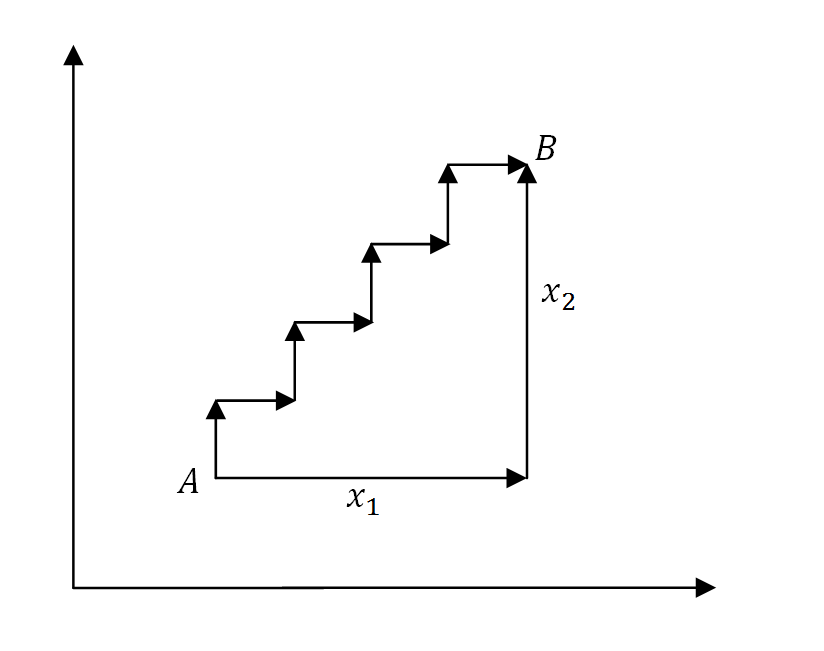
\includegraphics[scale=0.4]{l4_7.png}\end{center}
\begin{center}$\nu_M(\bar x) = |x_1|+...+|x_n|$ в $\mathbb{R}^n$, где $\bar x = (x_1,..., x_n)$\end{center}
\item Евклидова норма\\
(Для приближения)
\begin{center}
$\nu_E(\bar x) = \sqrt{|x_1|^2+...+|x_n|^2}$ в $\mathbb{R}^n$\end{center}
\item Норма максимума\\
(Уменьшает ошибку по всем координатам)\begin{center}
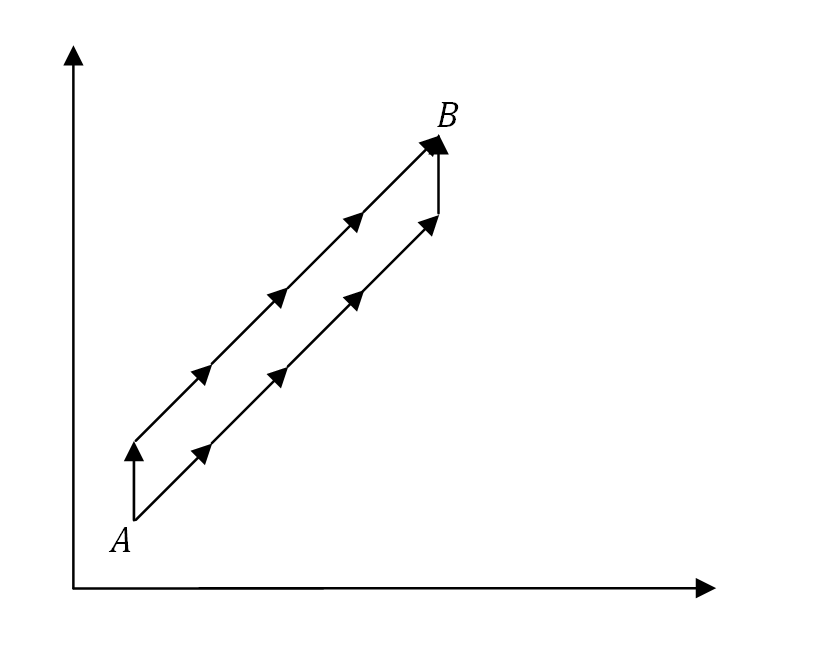
\includegraphics[scale=0.4]{l4_8.png}\end{center}
\begin{center}
$\nu_{max}(\bar x) = max\{|x_1|,...,|x_n|\}$ в $\mathbb{R}^n$\\\end{center}
\item Норма Гёльдера
\begin{center}$\nu_p(\bar x) = \sqrt[p]{|x_1|^p+...+|x_n|^p}$ в $\mathbb{R}^n$\\
$\nu_1(\bar x) = |x_1|+...+|x_n| = \nu_M(\bar x)$\\ 
$\nu_2(\bar x) = \sqrt{|x_1|^2+...+|x_n|^2} = \nu_E(\bar x)$\\
$\nu_{\infty}(\bar x) = \underset{p \to \infty}{lim}\sqrt[p]{\sum\limits_{i=1}^n |x_i|^p}$\end{center}
Если $|x_i| = max |x_i|$, то $\sqrt[p]{|x_i|^p} \to |x_i|$, получим:
\begin{center}$\nu_{\infty}(\bar x) = max \{|x_1|,...,|x_n|\} = \nu_{max}(\bar x)$\end{center}
\end{enumerate}
\textbf{Утверждение.}
В нормированном пространстве $V$ верно:\begin{enumerate}
\item $\forall \bar x, \bar y ~B_R(\bar x)$ равен $B_R(\bar y)$ (как геометрическая фигура).\\ 
$\blacktriangleright$ Пусть $\bar v = \bar y - \bar x$, тогда \begin{center} $B_R(\bar y) = \bar v + B_R(\bar x)$\end{center}
Ко всем точкам из $B_R(\bar x)$ прибавим одинаковый вектор $\bar v$.\begin{center}
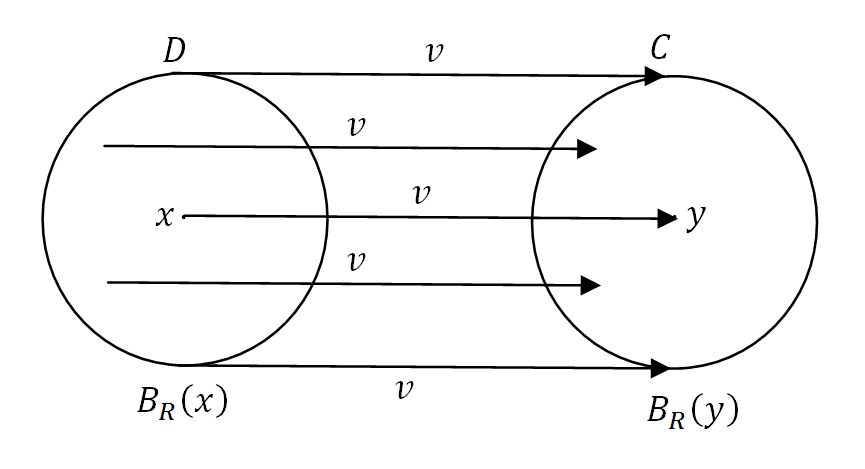
\includegraphics[scale=0.5]{l4_9.png}\\
$C \in B_R(y) \Leftrightarrow \nu(C-y) \leqslant R$\\
$\nu((C-(\bar y - \bar x))-\bar x) \leqslant R$\end{center}
То есть, $D = C-(\bar y-\bar x) \in B_R(\bar x). ~~\blacksquare$
\item Шары $B_R(\bar x)$ и $ B_{\alpha R}(\bar x)$, $\alpha > 0$ подобны с коэффициентом подобия $\alpha$.\\ 
$\blacktriangleright$ \begin{center}$\nu(x D) = \cfrac{1}{\alpha}\nu(x C)$\\
$D = x+xD = x+\cfrac{1}{\alpha}xC$\\
$\rho(D, x) = \nu(x D) = \cfrac{1}{\alpha}\nu(C-x) = \nu(\cfrac{1}{\alpha}(C-x))$\\
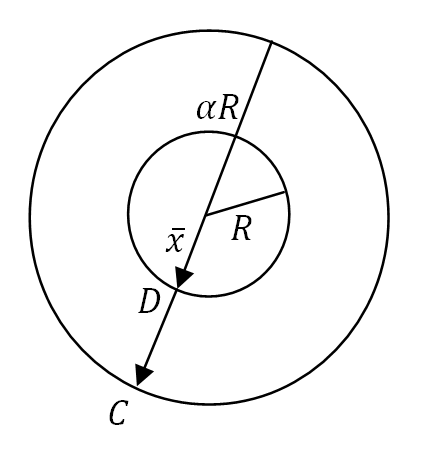
\includegraphics[scale=0.5]{l4_10.png}\\
$C \in B_{\alpha R}(x) \Leftrightarrow \nu(C-x) \leqslant \alpha R$\\
$\rho(D, x) = \nu(\cfrac{C-x}{\alpha}) \leqslant R$\end{center} То есть $D \in B_R(\bar x). ~~\blacksquare$
\end{enumerate}
~\\$\nu_p$ --- норма только при $p \geqslant 1$ (для невыпуклых --- неверно, не выполняется неравенство треугольника).\\
$B^p = B_1(\bar 0)$ относительно $\nu_p$.\begin{center}
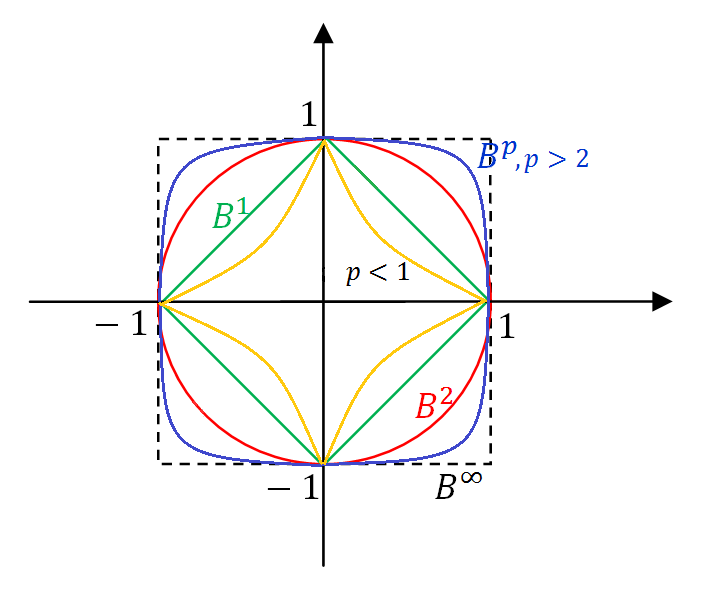
\includegraphics[scale=0.7]{l4_11.png}
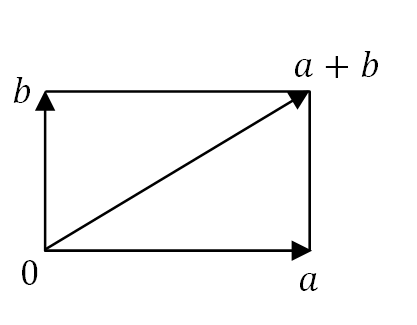
\includegraphics[scale=0.5]{l4_12.png}
\end{center}
\textbf{Пример 2.}\\
Для каких $R_1, R_2$ возможно $B_{R_1}(x) \subsetneq B_{R_2}(y)$?\\
\\
Если $R_2 > R_1$ --- возможно (даже при $x = y$).\\
При $R_1 = 5, R_2 = 4$ --- возможно (из предыдущего примера).\\
Докажем, что при $R_1 > R_2$ это не всегда верно, а именно: при $2R_2 > R_1$ - верно, а при $R_2 \leqslant \cfrac{R_1}{2}$ --- нет.\\
Рассмотрим случай $2R_2 = R_1$. \begin{center}
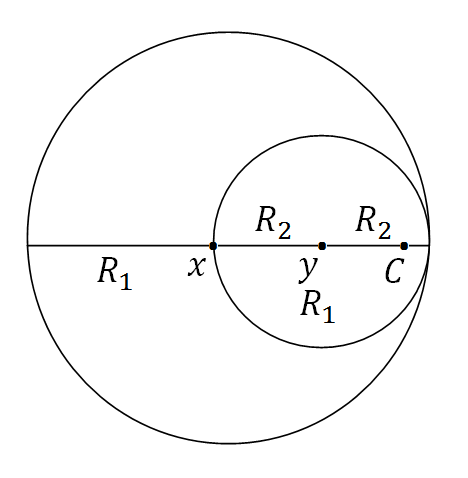
\includegraphics[scale=0.55]{l4_13.png}\end{center}
Тогда $B_{R_1}(x) = \{x, y, C\}$, $B_{R_2}(y) = \{x, y, C\}$, то есть $B_{R_1}(x) = B_{R_2}(y)$ --- множества совпадают, то есть уже не подходит.\\
\\
Рассмотрим случай, когда $R_1$ чуть меньше $2R_2$.\\
Тогда $B_{R_1}(x) = \{x, y\}$, $B_{R_2}(y) = \{x, y, C\}$, то есть $B_{R_1}(x) \subsetneq B_{R_2}(y)$ верно.\\
\\
Рассмотрим случай, когда $R_1$ чуть больше $2R_2$.\\
Тогда $B_{R_1}(x) = \{x, y, C\}$, $B_{R_2}(y) = \{x, y, C\}$, то есть, $B_{R_2}(y) \subseteq B_{R_1}(x)$, значит не подходит.\\
\\
Линейное пространство называется \textbf{евклидовым пространством}, если на нем задано скалярное произведение $g(x, y)$:\begin{enumerate}
\item $g(x, y) = g(y, x)$
\item $g(x_1+x_2, y) = g(x_1, y)+g(x_2, y)$
\item $g(\lambda x, y) = \lambda g(x, y)$
\item $g(x, x) \geqslant 0, g(x, x) = 0 \Leftrightarrow x = 0$
\end{enumerate}
В евклидовом пространстве есть стандартная норма $\parallel x \parallel = \sqrt{g(x, x)}$.\\
$L_2[0, 1]$ --- множество функций, квадрат которых интегрируем по Риману.\\
$(f, g) = \int\limits_0^1 f(x) \overline{g(x)}\,dx$\\
$\parallel f \parallel_2 = \sqrt{\int\limits_0^1 |f(x)|^2\,dx}$\\
\\
$x_n \to x$ $\textbf{сходится по норме}$ $\nu(x)$, если $\forall \varepsilon > 0 ~ \exists N(\varepsilon)~$, что $\forall n > N(\varepsilon)$ верно $~\nu(x_n - x) < \varepsilon$.\\ \\
\textbf{Пример 3.}\\
Является ли нормой на множестве непрерывно дифференцируемых функций $C^1[a, b]$ следующее выражение: \begin{center}$\mu(f) = \underset{a \leqslant x \leqslant b}{max}(|f(x)|+|f'(x)|)$ ?\end{center}
Да, так как выполняются все свойства нормы.\begin{enumerate}
\item $\mu(f) > 0$
\item $\mu(\lambda f) = \lambda \mu(f)$
\item $\mu(f+g) = max(|f+g|+|(f+g)'(x)|)$\\
$\mu(f)+\mu(g) = max(|f|+|g|+|f'|+|g'|)$\\
А так как $|f+g|\leqslant |f|+|g|$, то выполняется неравенство треугольника \\$\mu(f+g) \leqslant \mu(f) + \mu(g)$.\end{enumerate}
\textbf{Пример 4.}\\ Следует ли из сходимости по норме $\parallel f \parallel = \underset{a \leqslant x \leqslant b}{max} |f(x)|$ сходимость по $\mu(f)$, где \begin{center}$\mu(f) = \underset{a \leqslant x \leqslant b}{max}(|f(x)|+|f'(x)|)$ ?\end{center} Верно ли обратное?\\ \\
Докажем, что $f_k(x) \overset{\parallel f \parallel}{\rightarrow} f(x)$ и $f_k(x) \nrightarrow$ по $\mu(f)$.
\begin{center}
$f = x, f' = 1$\\
$f_k = \cfrac{1}{k}sin(xk^2)+x$\\
$|f-f_k| \leqslant \cfrac{1}{k} |sin(xk^2)| \leqslant \cfrac{1}{k} \to 0$, то есть, сходится по норме.\\
$f_k' = 1+k \cdot cos(xk^2)$\end{center}
$max \{|f(x)-f_k(x)|+|f'(x)-f_k'(x)|\} = max \{|\cfrac{1}{k}sin(xk^2)|+|1-1-k\cdot cos(xk^2)|\} \to \infty$, то есть, не сходится по $\mu(f)$.\\ \\
Обратное утверждение верно. При сходимости по $\mu(f)$ получим, что $|f(x)-f_k(x)|\to 0$, то есть сходится по норме.\\ \\
\noindent \textbf{Домашнее задание 4}\begin{enumerate}
\item
$B(x, y) = \{x^2+axy+4y^2 \leqslant 1\}$\\
При каких $a$ на множестве $\mathbb{R}^2$ существует норма $\nu$ такая, что $B(x, y)$ --- единичный шар относительно нее? \\Найдите в этом случае
\[\nu \begin{pmatrix}
2 \\
1\\
\end{pmatrix}\]
\item
Будет ли метрикой на $\mathbb{R}$ функция $\rho(x, y) =$\begin{enumerate}
\item $|x^2-y^2|$
\item $sin(x-y)$
\item $|e^x-e^y|$
\end{enumerate}
\item
Существует ли убывающая последовательность непустых замкнутых ограниченных множеств с пустым пересечением (в произвольном метрическом пространстве)?
\item
Доказать, что шар в нормированном пространстве является выпуклым множеством. То есть доказать, что если $x, y$ принадлежат шару, то и весь отрезок $[x, y]$ принадлежит шару.\end{enumerate}
\section *{Лекция 5}
\noindent Множество \textbf{замкнутое}, если оно включает свою границу.\\ \\
$V$ --- линейное пространство, $\nu$ --- \textbf{норма} на $V$ ($\nu : V \to$ $\mathbb{R}$ $\geqslant 0$) если:\begin{enumerate}
\item $\nu(\bar x) > 0$, $\bar x \neq \bar 0$, $\nu(\bar 0) = \bar 0$
\item $\nu(\alpha \bar x) = |\alpha|\nu(\bar x)$
\item $\nu(\bar x + \bar y) \leq \nu(\bar x) + \nu(\bar y)$ для $\forall x, y \in V, \forall \alpha$\\
$\nu (x) = |x|$\end{enumerate}
~\\
$\mathbb{R}^2$, $\nu(\bar x) - ?,~ \nu(\bar v ) - ?$\\
$B_1^{\nu}(\bar 0) = B_1^{\nu}$\begin{center}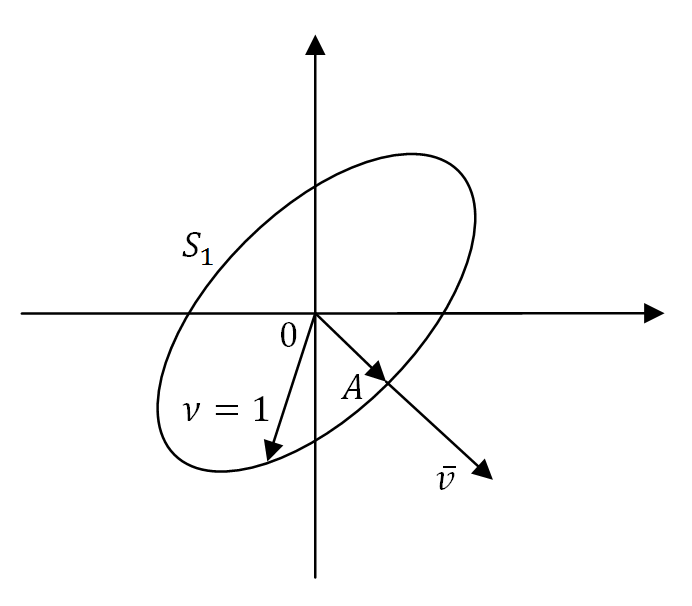
\includegraphics[scale=0.6]{l5_2.png}\\
$A = $ луч $ \cap S_1$, $~S_1$ --- граница\\
$\nu(OA) = 1$\\
$\nu(v) = \lambda \nu(OA) = \lambda$, если $v = \lambda OA, \lambda = \cfrac{|v|}{|OA|}$
\end{center}
\textbf{Лемма.}
Пусть $\nu_1, \nu_2$ --- две нормы на $\mathbb{R}^n$, тогда существует такое $c>0$, что любой шар одной нормы содержится в другом шаре другой нормы.\begin{center}
$B_R^{\nu_1} \subset B_{cR}^{\nu_2}$.\end{center}
\textbf{Следствие.}
Любые две нормы в $\mathbb{R}^n$ эквивалентны, то есть для $\forall~ \nu_1, \nu_2 ~\exists~ c_1, c_2$, что для $\forall ~\bar x$ верно $c_1\nu_1(x) \leqslant \nu_2(x) \leqslant c_2\nu_1(x)$.\\
\\
\textbf{Следствие.}
Шар $B_1^{\nu_1}$ --- ограниченное множество, то есть $B_R^{\nu_1} \subset \{ \bar x ~|~ |\bar x| \leqslant M \} = B_M^E$ (евклидов шар).\begin{center}
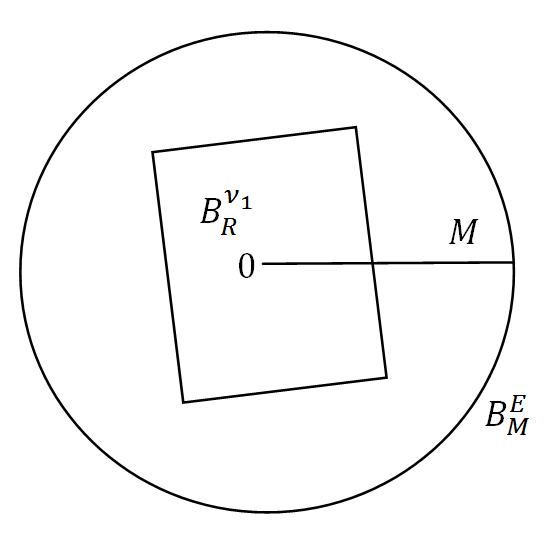
\includegraphics[scale=0.5]{l5_4.png}\end{center}
$\blacktriangleright \nu_2 = $евклидова длина, $M=cR ~~ \blacksquare$\\
\\
\textbf{Доказательство леммы.}\\
$\blacktriangleright$ 
Пусть \[\bar x = \begin{pmatrix}
x_1 \\
...\\
x_n \\
\end{pmatrix} = x_1 \bar e_1 +...+x_n \bar e_n \in B_1^{\nu_1} (R = 1)\]
$\nu_2(\bar x) = \nu_2 (x_1 \bar e_1 +...+x_n \bar e_n) \leqslant \nu_2(x_1e_1)+...+\nu_2(x_ne_n) = |x_1|\nu_2(e_1)+...+|x_n|\nu_2(e_n) \leqslant \\ \leqslant \underset{i=1,...,n}{max} \{\ |x_i|\}$.\begin{center}
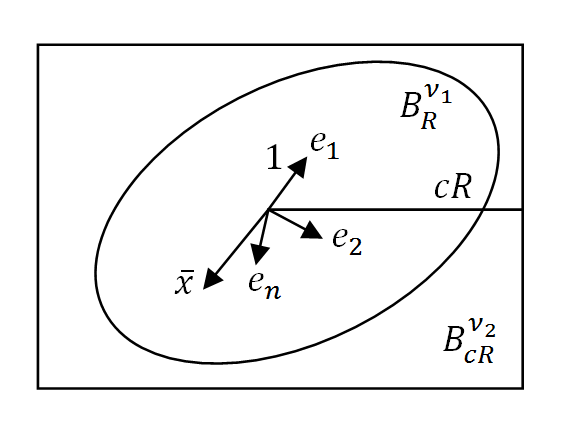
\includegraphics[scale=0.5]{l5_5.png}\end{center}
Пусть $|\bar x|_{\infty} = \underset{i=1,...,n}{max}|x_i|, ~M = \underset{i=1,...,n}{max}\nu_2(e_i)$, тогда $\nu_2(x) \leqslant |\bar x|_{\infty}nM$, то есть $B_R^{\nu_1} \subset B_{cR}^{|\cdot |_{\infty}}, c = nM$.\\
Доказали, что любой единичный шар можно поместить в квадрат со стороной $cR$.\\
\\
Если $|x|_{\infty} \leqslant \cfrac{1}{nM}$, то $\nu_2(x) \leqslant 1, x \in B_1^{\nu_2}$.\begin{center} 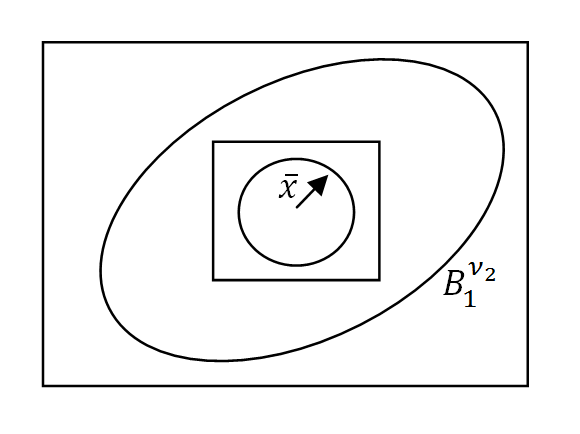
\includegraphics[scale=0.5]{l5_6.png}\end{center}
Внутри любого единичного шара существует квадрат, то есть существует куб, который содержит его целиком. Осталось доказать, что шар --- ограниченное множество. Докажем от противного.\begin{center}
$B_1^{\nu} = \{x | \nu(\bar x) \leqslant 1\}$\end{center}
Пусть существует $\{x^1, x^2,...\}: \{|x^1|, |x^2|,...\} \rightarrow +\infty$, тогда она существует, если $B_1^{\nu}$ неотрицательное множество.\begin{center}
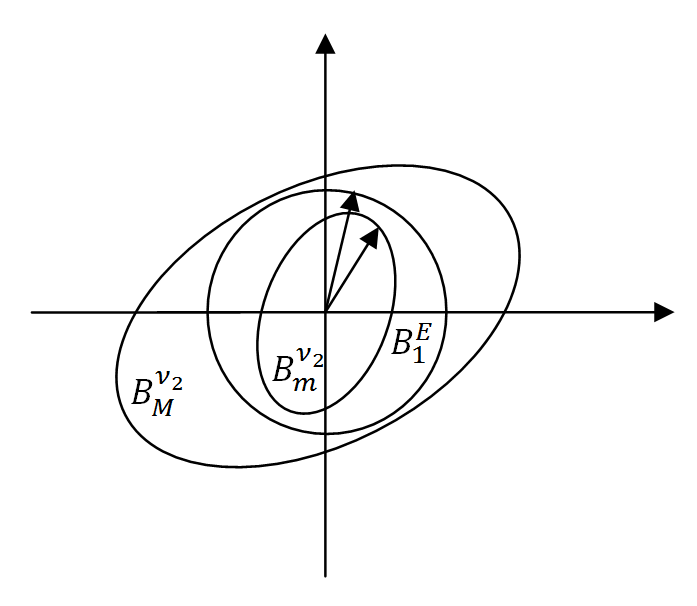
\includegraphics[scale=0.55]{l5_7.png}
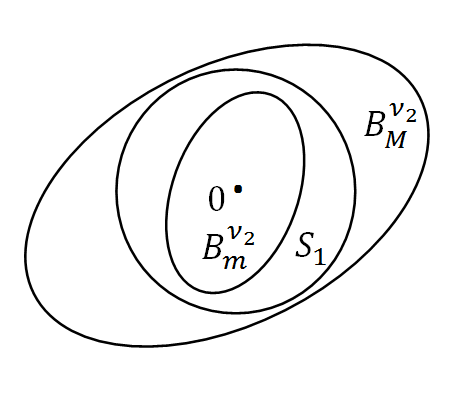
\includegraphics[scale=0.55]{l5_9.png}
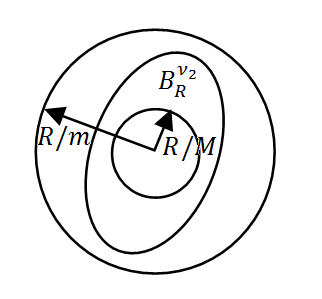
\includegraphics[scale=0.65]{l5_8.png}\end{center}
$m \leqslant \nu_2(B_1^E) \leqslant M$, где $m > 0, ~M$ --- ограниченное множество, тогда (так как все шары подобны):\\ \\
$
\left\{  
\begin{array}{lcl}  
    B_m^{\nu_2} \subset B_1^E \subset B_M^{\nu_2} \\  
    B_R^{\nu_2} \subset B_{R/m}^E \\
    B_{R/M}^E \subset B_R^{\nu_2}\\
\end{array}   
\right.  
$
\\
$\blacksquare$
\\ 
\textbf{Теорема Минковского.}
Множество $B \subset \mathbb{R}^n$ является единичным шаром $B_1^{\nu}$ относительно какой-либо нормы $\nu$ тогда и только тогда, когда $B$:\begin{enumerate}
\item замкнуто
\item ограничено ($B \subset B_M^E$)
\item содержит окрестность нуля (то есть $B \supset B_m^E$)
\item выпукло
\item центрально симметрично (если $\bar x \in B$, то и $-\bar x \in B$)
\end{enumerate}
\textbf{Пример 1.}\\
$B = \{x^2+axy+4y^2 \leqslant 1\}$\\
Существует ли такая норма $\nu$, что $B$ --- единичный шар относительно нее ($B = B_1^{\nu}$)?\\
\begin{center}
$
\begin{pmatrix}
1 & \cfrac{a}{2}\\
\cfrac{a}{2} & 4
\end{pmatrix}
$
\\ ~\\
$\vartriangle_1 = 1 > 0$\\
$\vartriangle_2 = 4 - \cfrac{a^2}{4} > 0$\end{center}
То есть это эллипс, все 5 свойств из предыдущей теоремы выполняются, значит при $|a| < 4 B$ --- единичный шар относительно нормы.\begin{center}
$\vartriangle_1 = 1 > 0$\\
$\vartriangle_2 = 4 - \cfrac{a^2}{4} < 0$\end{center}
В этом случае множество не будет замкнутым, то есть не выполняются все свойства из предыдущей теоремы, значит в этом случае $B$ не будет единичным шаром относительно нормы.\\
При $\vartriangle_2 = 0$: $ a = \pm 4$ и $x^2 \pm 4xy+4y^2 \leqslant 1$, $(x \pm 2y)^2 \leqslant 1$. В этом случа получим множество между двумя параллельными прямыми, которое является незамкнутым, то есть в этом случае $B$ тоже не будет единичным шаром относительно нормы.\\
Получили, что $B = B_1^{\nu}$ только при $|a| < 4$.\\
\\
$V$ --- \textbf{евклидово пространство со скалярным произведением}, если задана $V \times V \rightarrow \mathbb{R}$, то есть, на нем задано скалярное произведение $(\bar u, \bar v) \in \mathbb{R}$ такое, что для пространств над $\mathbb{R}$ выполнено:\begin{enumerate}
\item $(u, v) = (v, u)$
\item $(u'+u'', v) = (u', v)+(u'', v)$
\item $\alpha (u, v) = (\alpha u, v) = (u, \alpha v), \alpha \in \mathbb{R}$
\item $(u, u) > 0, u \neq \bar 0~ ((u, u) = 0 \Leftrightarrow u=0)$
\end{enumerate}
Обозначение скалярного произведения: $(u, v)=<u, v>=<u~|~v>$.\\ \\
Длина вектора --- это $|v| = \sqrt{(v, v)} \geqslant 0$ (норма).\\
$\blacktriangleright$ \begin{center}$|\alpha v| = \sqrt{(\alpha v, \alpha v)} = \sqrt{\alpha^2 (v, v)} = |\alpha||v|$\\
$|v| > 0$, при $v \neq \bar 0$\\
$|u+v| \leqslant |u|+|v| ~~\blacksquare$\end{center}
$$cos \widehat{(u, v)} = \cfrac{(u, v)}{|u||v|}, u, v \neq \bar 0$$\\
$V$ --- \textbf{эрмитово пространство со скалярным произведением}, если задана $V \times V$ $\rightarrow \mathbb{C}$, то есть, на нем задано скалярное произведение $(\bar u, \bar v) \in \mathbb{C}$ такое, что для пространств над $\mathbb{C}$ выполнено:\begin{enumerate}
\item $(u, v) = \overline{(v, u)}$
\item $(u'+u'', v) = (u', v)+(u'', v)$
\item $\alpha (u, v) = (\alpha u, v) = (u, \alpha v), \alpha \in \mathbb{C}$
\item $\forall u~ (u, u) \geqslant 0, (u, u) = 0 \Leftrightarrow u=0$
\end{enumerate}
Как по норме $|w|$ восстановить скалярное произведение $(u, v)$?
\begin{center}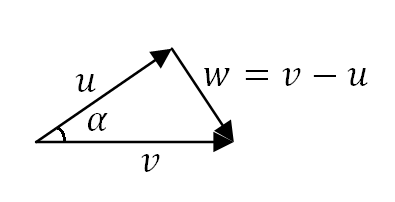
\includegraphics[scale=0.55]{l5_10.png}\\
$|w|^2 = (w, w) = (v-u, v-u) = (v, v) - (u, v) - (v, u) + (u, u) = |v|^2 - 2(u, v) + |u|^2$\end{center}
То есть, $(u, v) = \cfrac{1}{2}(|v|^2 + |u|^2 - |v-u|^2)$.\\
\\
\textbf{Теорема (тождество параллелограмма).}
Пусть $V$ --- нормированное пространство с нормой $|v|$. На $V$ существует такое скалярное произведение, что $|v| = \sqrt{(v, v)}$ в том и только том случае, когда в $V$ выполняется тождество параллелограмма:\begin{center}
$\forall a, b~ |a+b|^2 + |b-a|^2 = 2(|a|^2 + |b|^2)$\end{center}
При $c = a+b, d = b-a:$ \begin{center}$c^2+d^2 = 2(a^2+b^2)$\\
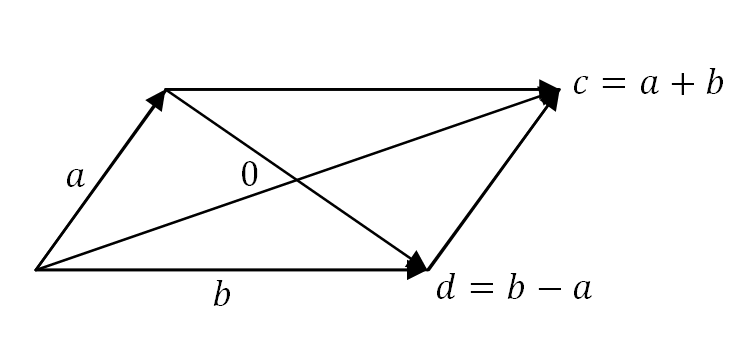
\includegraphics[scale=0.55]{l5_11.png}\end{center}
$\blacktriangleright $ Если для $\forall v ~|v| = \sqrt{<v, v>}$, то $|a+b|^2+|b-a|^2 = <a+b, a+b> + <b-a, b-a> = \\=<a, a> + 2<a, b> + <b, b> +<b, b> - 2<a, b> + <a, a> = 2(|a|^2 + |b|^2)~~ \blacksquare$\\
\\
$H$ --- \textbf{гильбертово пространство}, если на нем задано скалярное произведение и оно является полным (относительно метрики, порожденной скалярным произведением).\\
\\
Набор $\{ \varphi_0, \varphi_1,...,\varphi_n,...\}^{-e}$ называется \textbf{ортогональной системой}, если \\$(\varphi_i, \varphi_j) = \delta_j^i = 
\left\{  
\begin{array}{lcl}  
    1, i = j \\  
    0, i \neq j \\
\end{array}   
\right.  
$\\
Формально хотим представить $f = \sum\limits_{n=0}^{\infty} c_n \varphi_n$.\begin{center}
$(f, \varphi_j) = c_j(\varphi_j, \varphi_j)$\\ 
$(\varphi_j, \varphi_j) = 1$\\ 
$c_j = \cfrac{(f, \varphi_j)}{\parallel \varphi_j \parallel^2} = (f, \varphi_j)$\end{center} $c_j$ --- коэффициенты Фурье по ортогональной системе.\\ \\
\textbf{Теорема.}
Если $\varphi_j$ --- ортогональная система, тогда следующие условия эквивалентны:\begin{enumerate}
\item система $\{\varphi_j\}$ является базисом, то есть $f = \sum\limits_{n=0}^{\infty}c_n \varphi_n$
\item выполнение равенства Парсеваля $\parallel f \parallel^2 = \sum\limits_{n=0}^{\infty}c_k^2$
\item система является полной, то есть $\exists y \neq 0: (\varphi_j, y) = 0$
\end{enumerate}
Хотим приблизить $f$ и минимизировать $\parallel f - \sum\limits_{k=0}^n \alpha_k \varphi_k \parallel \to min$.\\
$(f - \sum\limits_{k=0}^n \alpha_k \varphi_k, f - \sum\limits_{k=0}^n \alpha_k \varphi_k) =$ (так как система ортогональна) $= (f, f) - 2\sum\limits_{k=0}^n \alpha_k (f, \varphi_k) +\\+\sum\limits_{k=0}^n \alpha_k^2 (\varphi_k, \varphi_k) = (c_k=(f, \varphi_k),~ (\varphi_k, \varphi_k)=1) = \parallel f \parallel^2 + \sum\limits_{k=0}^n (\alpha_k - c_k)^2 - \sum\limits_{k=0}^n c_k^2$\\
Выбором $\alpha$ хотим минимизировать, минимальная норма будет там, где совпадают $\alpha_k = c_k$.\\
\\
$a = \{1, x, x^2,..., x^n\}$ --- пространство $\mathbb{R}_{n+1}$ многочленов степени $\leqslant n$ на $[-1, 1]$, где скалярное произведение $\int\limits_{-1}^1 f(x)g(x)\,dx$. Применим к $a$ процесс Грама-Шмидта, получим $b$.\begin{center}
$a \to b = \{P_0(x)=1\}$\end{center}
\textbf{Многочлены Лежандра:} \begin{center}$P_k(x) = \cfrac{1}{2^k k!}\cfrac{d^k}{dx^k}((x^2-1)^k)^{(k)}, k=1,..,n$\end{center}\begin{description} 
\item[k=0:] $P_0(x)=1$
\item[k=1:] $P_1(x)=\cfrac{1}{2}(x^2-1)'=x$
\item[k=2:] $P_2(x)=\cfrac{1}{8}((x^2-1)^2)''=\cfrac{1}{8}(4x(x^2-1)'=\cfrac{3x^2-1}{2}$
\item[k=3:] $P_3(x)=\cfrac{1}{48}((x^2-1)^3)'''=\cfrac{1}{2}(5x^3-3x)$\end{description}
$\parallel P_1(x) \parallel = \sqrt{\int\limits_{-1}^1 x \cdot x\,dx} = \sqrt{\cfrac{2}{3}}$\\
\\
\textbf{Домашнее задание 5}\begin{enumerate}
\item
\begin{enumerate}
\item Проверить ортогональность $P_2(x)$ и $P_3(x)$ относительно $<f, g> =\\= \int\limits_{-1}^1 f(x)g(x)\,dx$.
\item Найти $\parallel P_n(x) \parallel$.
\end{enumerate}
\item
Найти $\alpha_0, \alpha_1, \alpha_2$ на $[-1, 1]$: $\parallel f - \sum\limits_{k=0}^2 \alpha_kP_k(x) \parallel \to min$, $d_j=\cfrac{(f, \varphi_j)}{\parallel \varphi_j \parallel^2} = (f, \varphi_j)$, где $P_k(x)=\cfrac{1}{2^k k!}\cfrac{d^k}{dx^k}((x^2-1)^k)^{(k)},~k=1,\cdots, n$ --- многочлены Лежандра.
\begin{enumerate}
\item $f_1(x)=xe^{-x}$
\item $f_2(x)=x^3$\\
\end{enumerate}
\item
Выразить скалярное произведение через длину вектора в эрмитовом пространстве.\end{enumerate}
\section *{Лекция 6}
\noindent \textbf{Многочлены Чебышева 1 рода.}
\begin{center}
$T_0(x) = 1$ \\
$T_1(x) = x$\\
$\cdots$\\
$T_n(x) = 2xT_{n-1}(x)-T_{n-2}(x), n\geqslant 2$
\end{center} 
\begin{center}
\begin{tabular}{|l|l|}
\hline
\textbf{n} & \textbf{T(n)} \\ \hline
0 & 1 \\ \hline
1 & $x$ \\ \hline
2 & $2x^2-1$ \\ \hline
3 & $4x^3-3x$ \\ \hline
4 & $8x^4-8x^2+1$ \\ \hline
5 & $16x^5-20x^3+5x$ \\ \hline
6 & $32x^6-48x^4+18x^2-1$ \\ \hline
7 & $64x^7-112x^5+56x^3-7x$ \\ \hline
8 & $128x^8-256x^6+160x^4-32x^2+1$ \\ \hline
9 & $256x^9-576x^7+432x^5-120x^3+9x$ \\ \hline
10 & $512x^{10}-1280x^8+1120x^6-400x^4+50x^2-1$ \\ \hline
\end{tabular}
\end{center}
Для главного члена в формуле $T_n(x)=2^{n-1}x^n+..., n\geqslant 1$.\\
$\blacktriangleright$ По индукции:\begin{center}
$T_{n+1}(x)=2xT_n(x)-T_{n-1}(x)=2x2^{n-1}x^n+\cdots-2^{n-2}x^{n-1}=2^nx^{n+1}+...$ верно для $n+1. ~~\blacksquare$\end{center}
Графики многочленов $T_0(x),~ T_1(x),~ T_2(x)$:\begin{center}
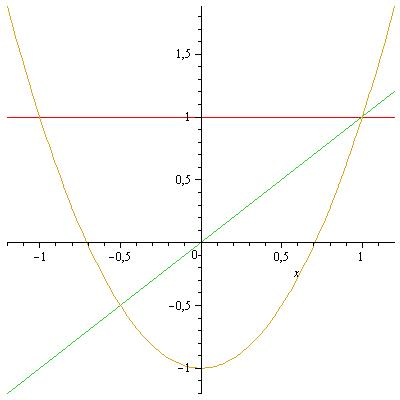
\includegraphics[scale=0.5]{T0T1T2.jpg} \end{center}
Графики многочленов $T_3(x),~ T_4(x),~ T_5(x)$:\begin{center}
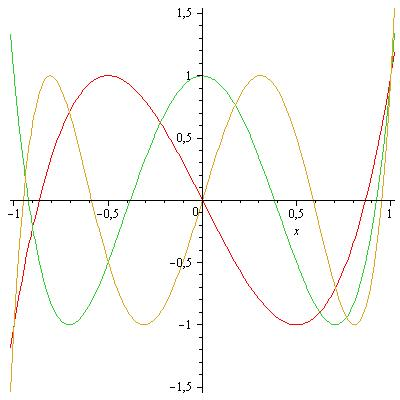
\includegraphics[scale=0.5]{T3T4T5.jpg} \end{center}	
График многочлена $T_{10}(x)$:\begin{center}
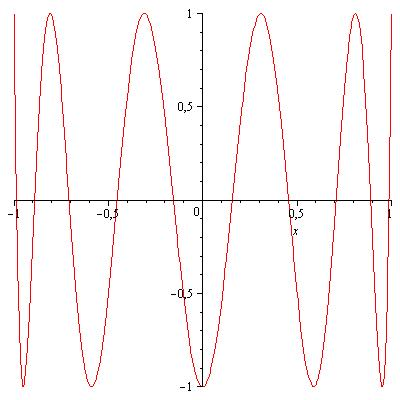
\includegraphics[scale=0.5]{T10.jpg} \end{center} 
\textbf{Теорема.}
$T_n(cos \varphi)=cos(n\varphi)$\\
\\
\textbf{Следствие.}
$T_n(x)=cos(n ~ arccos~x)$ при $ x \in [-1, 1]$\\
\\
\textbf{Следствие.}
$T_n(x)=\cfrac{(x+\sqrt{x^2-1})^n+(x-\sqrt{x^2-1})^n}{2}$ при $ |x| \geqslant 1$
\begin{center}
$x=cos~\varphi$\\
$cos(2\varphi)=2x^2-1$\\
$cos(3\varphi)=4x^3-3x$\\
$\cdots$\\
$cos(n\varphi)+cos((n-2)\varphi)=2cos \bigg(\cfrac{n+n-2}{2}~\varphi \bigg)cos \bigg(\cfrac{n-n+2}{2}~\varphi \bigg)=2cos((n-1)\varphi)cos \varphi$\\
~\\
$T_n(x)=0 \Leftrightarrow cos(n\varphi)=0 \Leftrightarrow n\varphi=\pi k +\cfrac{\pi}{2}=\pi\cfrac{(2k+1)}{2}, \varphi \in [0, \pi]$\\
$\varphi=\pi\cfrac{(2k+1)}{2n} \Leftrightarrow x=arccos \bigg(\cfrac{2k+1}{n}~\pi \bigg)$\end{center}
\textbf{Многочлены Чебышева 2 рода.}
\begin{center} $U_n(x)=\cfrac{1}{n+1}T_{n+1}'(x)$ при $ n \geqslant 0$\end{center}
\begin{center}
\begin{tabular}{|l|l|}
\hline
\textbf{n} & \textbf{U(n)} \\ \hline
0 & 1 \\ \hline
1 & $2x$ \\ \hline
2 & $4x^2-1$ \\ \hline
3 & $8x^3-4x$ \\ \hline
4 & $16x^4-12x^2+1$ \\ \hline
5 & $32x^5-32x^3+6x$ \\ \hline
6 & $64x^6-80x^4+24x^2-1$ \\ \hline
7 & $128x^7-192x^5+80x^3-8x$ \\ \hline
8 & $256^8-448x^6+240x^4-40x^2+1$ \\ \hline
9 & $512x^9-1024x^7+672x^5-160x^3+10x$ \\ \hline
10 & $1024x^{10}-2304x^8+1792x^6-560x^4+60x^2-1$ \\ \hline
\end{tabular}
\end{center} 
Графики многочленов $U_0(x),~ U_1(x),~ U_2(x)$:\begin{center}
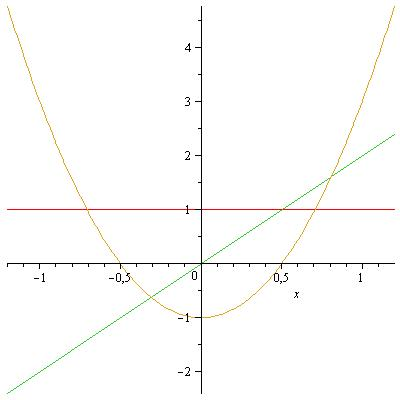
\includegraphics[scale=0.5]{U0U1U2.jpg} \end{center}
Графики многочленов $U_3(x),~ U_4(x),~ U_5(x)$:\begin{center}
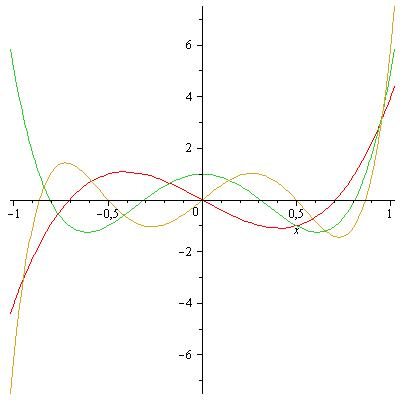
\includegraphics[scale=0.5]{U3U4U5.jpg} \end{center}	
График многочлена $U_{10}(x)$:\begin{center}
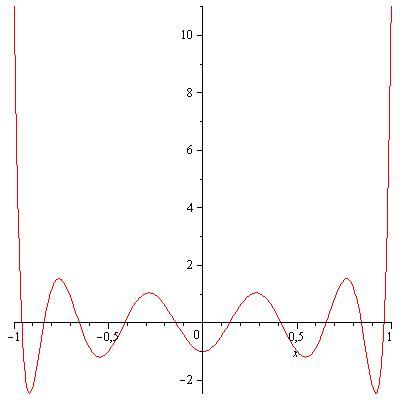
\includegraphics[scale=0.5]{U10.jpg} \end{center}
\textbf{Теорема.}
$U_{n-1}(cos \varphi)sin \varphi = sin(n \varphi)$\\
\\
\textbf{Теорема.}
$U_n(x)=\cfrac{(x+\sqrt{x^2-1})^{n+1}+(x-\sqrt{x^2-1})^{n+1}}{\sqrt{x^2-1}}$ при $ |x| \leqslant 1$
\begin{center}
$sin(n\varphi)=sin\varphi ~ U_{n-1}(x),$ $ U_{n-1}=\cfrac{sin(n\varphi)}{sin \varphi}$\\
$U_{n-1}(x) = 0 \Leftrightarrow n\varphi=\pi k,$ $\varphi=\cfrac{\pi k}{n}$
\end{center}
\textbf{Свойство.}
Старший коэффициент многочлена $T_n(x)$ равен $2^{n-1}$, а старший коэффициент многочлена $U_n(x)$ равен $2^n$.\\
\newpage
\noindent \textbf{Теорема.}\begin{enumerate}
\item При $n \geqslant 1$ многочлен $T_n(x)$ имеет на отрезке [-1, 1] ровно $n$ корней $cos\cfrac{(2k-1)\pi}{2n}, k=1,..,n.$
\item Корни многочлена $U_n(x)$ (они же - экстремумы многочлена $T_{n+1}(x)$) также принадлежат отрезку [-1, 1]: это числа $cos\cfrac{\pi k}{n+1}, k=1,...,n.$
\end{enumerate}
\textbf{Следствие.}\begin{center}
$T_n(x)=2^{n-1} \bigg(x-cos~\cfrac{\pi}{2n}\bigg) \bigg(x-cos~\cfrac{3\pi}{2n}\bigg)\cdots \bigg(x-cos(2n-1)\cfrac{\pi}{2n} \bigg)$\\
~\\
$U_n(x)=2^n \bigg(x-cos~\cfrac{\pi}{n+1}\bigg) \bigg(x-cos~\cfrac{2\pi}{n+1} \bigg)\cdots \bigg(x-cos ~n\cfrac{\pi}{n+1}\bigg)$\end{center}
\textbf{Следствие.}
Многочлен $T_n(x)$ степени $n$ на отрезке $[-1, 1]$ достигает своих экстремальных значений, равных 1 и -1 в $n+1$ точке, включая концы отрезка.\\ \\
Пример: $n=6$ (график многочленов $T_6(x)$ и $U_5(x)$).\begin{center}
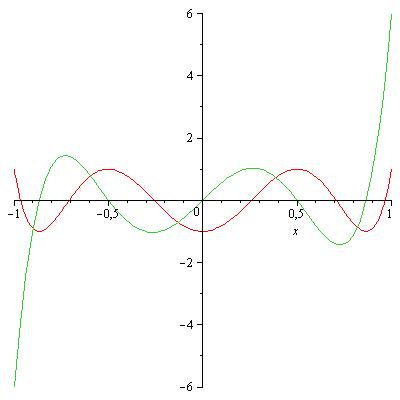
\includegraphics[scale=0.5]{T6U5.jpg} \end{center}
\textbf{Уклонение от нуля.}\\
Пусть $f$ --- функция на отрезке $[-1, 1]$. Как измерить, насколько она далека от нуля?\\
Норма Чебышева \begin{center}$|f|_0=\underset{[-1, 1]}{max}|f(x)|$ (максимум модуля на данном отрезке)\end{center}
и \begin{center}$|f|_1=\int\limits_{-1}^1 |f(x)|\,dx$ (площадь под графиком на данном отрезке).\end{center}
Пусть $|| \cdot ||$ --- норма на пространстве многочленов (например, одна из двух упомянутых). Многочлен $f(x)=x^n+\cdots$ степени $n$ со старшим коэффициентом 1 называется наименее уклняющимся от нуля относительно данной нормы, если для любого другого такого многочлена $g(x)=x^n+\cdots$ всегда $\parallel f \parallel \leqslant \parallel g \parallel$.\\
\\
\textbf{Пример 1.}\\
Относительно нормы Чебышева $|f|_0$ уклонение от нуля многочлена $\widetilde{T_3}(x)=\cfrac{1}{4}~T_3(x)=\\=x^3-\cfrac{3}{4}x$ равно\begin{center} $|\cfrac{1}{4}~T_3(x)|_0=\cfrac{1}{4}~|T_3(x)|_0=\cfrac{1}{4}$~,\end{center} а, например, для многочлена $x^3$ имеем $|x^3|_0=1$.\\ \\
\textbf{Теорема.}\begin{enumerate}
\item (Чебышев) Наименее уклоняющимся от нуля на отрезке $[-1, 1]$ относительно нормы Чебышева\begin{center} $|f|_0=\underset{[-1, 1]}{max}|f(x)|$ \end{center} является многочлен $\widetilde T_n(x)=\cfrac{1}{2^{n-1}}T_n(x)$.
\item (Коркин, Золотарев) Наименее уклоняющимся от нуля на отрезке $[-1, 1]$ относительно нормы \begin{center}$|f|_1=\int\limits_{-1}^1 |f(x)|\,dx$ \end{center} является многочлен $\widetilde U_n(x)=\cfrac{1}{2^{n-1}}U_n(x).$
\end{enumerate}
Дано: многочлен $f(x)=x^n+\cdots$ на $[-1, 1]$\\
Надо найти: $g(x)=c \cdot x^n+\cdots$, приближающий $f(x)$ в смысле $|\cdots|_1$ или $|\cdots|_0$.\\
$g \approx f \Leftrightarrow f-g$ --- многочлен, наименее уклоняющийся от нуля, то есть $f(x)-g(x) = \widetilde U_n(x)$ или $\widetilde T_n(x)$.\\
\\
\textbf{Следствие.}
Наименее уклоняющийся от нуля на отрезке $[a, b]$ многочлен степени $n$ относительно нормы Чебышева на этом отрезке $|f|_0=\underset{[a, b]}{max}|f(x)|$ --- это \begin{center}$\overline T_n(x) = \cfrac{(b-a)^n}{2^{2n-1}}T_n \bigg(\cfrac{2x-(b+a)}{b-a} \bigg)$.\end{center}
Идея доказательства: сделать замену переменных $y=\cfrac{2x-(b+a)}{b-a}$, где $x\in [a, b]$, а $y \in [-1, 1]$, и свести задачу к поиску многочлена, наименее уклоняющегося от нуля на отрезке $[-1, 1]$.\\
\\
\textbf{Пример 2.}\\
Наименее уклоняющийся от нуля на отрезке $[0, 1]$ многочлен степени $n$ --- это многочлен $$\overline T_n(x)=\cfrac{1}{2^{2n-1}}T_n(2x-1).$$\\
В частности, $\overline T_2(x)=\cfrac{1}{2^{4-1}}T_2(2x-1)=\cfrac{1}{8}(2(2x-1)^2-1)=x^2-x+\cfrac{1}{8}$.\\
\noindent Скалярное произведение непрерывных функций на отрезке $[-1, 1]:$ $$<f, g>=\int\limits_{-1}^1 \cfrac{f(x)g(x)}{\sqrt{1-x^2}}\,dx.$$\\
Ему соответствует норма: $$\parallel f \parallel=\sqrt{<f,f>}=\sqrt{\int\limits_{-1}^1 \cfrac{f(x)^2}{\sqrt{1-x^2}}\,dx}.$$\\
Соотношения ортогональности: $$<T_m, T_n>=
\left\{  
\begin{array}{ccl}  
    0,& m\neq n\\
    \cfrac{\pi}{2},& m=n\neq 0\\
    \pi,& m=n=0\\  
\end{array}   
\right.  
$$
\\
Наилучшее приближение функции $f$ многочленом степени $\leqslant n:$ $$\widetilde f(x)=\sum\limits_{i=0}^n\cfrac{<T_i, f>}{<T_i, T_i>}T_i(x)$$\\
\textbf{Пример 3.}\\
$f(x)=x^3$ на $[-1, 1]$ разложить в ряд по многочленам Чебышева.
\begin{center}
\begin{tabular}{|l|l|}
\hline
T & K \\ \hline
1 & 1 \\ \hline
$x$ & $x$ \\ \hline
$2x^2-1$ & $x^2-\frac{1}{2}$ \\ \hline
$4x^3-3x$ & $x^3-\frac{3}{4}x$\\ \hline
\end{tabular}
\end{center}
$K=\widetilde T$ --- отнормированные значения.\begin{center}
$f(x)=x^3=\widetilde T_3+\cfrac{3}{4}\title{T_1}$\\
$x^3=\sum\limits_{i=0}^3\cfrac{<\widetilde T_i, f>}{<\widetilde T_i, \widetilde T_i>}\widetilde T_i$
\end{center}
\textbf{Пример 4.}\\
$\parallel x^3-P_2(x) \parallel_\infty \to min$ на отрезке $[-1, 1]$ приблизить многочленом, где $P_2(x)$ --- любой многочлен второй степени.\\
\\
Для отрезка $[-1, 1]$: \begin{center}
$x^3-P_2(x)=\widetilde T_3(x)$\\
$x^3-x^3+\cfrac{3}{4}x=P_2(x)$\\
$P_2(x)=\cfrac{3}{4}x$
\end{center}
\textbf{Пример 5.}\\
$\parallel x^3-P_2(x) \parallel_\infty \to min$ на отрезке $[2, 3]$ приблизить многочленом, где $P_2(x)$ --- любой многочлен второй степени.\\
\begin{center}
$x^3-P_2(x)=\overline T_3(x)$\\
$P_2(x)=x^3-\overline T_3(x)$\\
\end{center}
Вычислим $\overline T_3(x)$ по формуле $\overline T_n(x) = \cfrac{(b-a)^n}{2^{2n-1}}T_n \bigg(\cfrac{2x-(b+a)}{b-a} \bigg)$.\\
\begin{center}
$\overline T_3(x)=\cfrac{(b-a)^3}{2^5}T_3 \bigg(\cfrac{2x-(b+a)}{b-a}\bigg) =\cfrac{1}{2^5}T_3(2x-5)=\cfrac{1}{32}(4(2x-5)^3-3(2x-5))=$\\
$=\cfrac{1}{32}(4(8x^3-60x^2+150x-125)-6x+15)=\cfrac{1}{32}(32x^3-240x^2+600x-500-6x+15)=$\\
$=x^3-7.5x^2+18.5625x-15.15625$\end{center}
Подставив $\overline T_3(x)$ в $P_2(x)$, получим:
$$P_2(x)=x^3-\overline T_3(x)=7.5x^2-18.5625x+15.15625$$ 
\textbf{Пример 6.}\\
Если $U_n(x)=\cfrac{1}{n+1} \Big(T_{n+1}(x)\Big)'$ будет ли верно $U_{n+1}(x)=2xU_n(x)-U_{n-1}(x)$ ?
\begin{description} 
\item[n:]
$$\cfrac{1}{n+1}\Big(2xT_n(x)-T_{n-1}(x)\Big)'=\cfrac{1}{n+1}\Big(2T_n(x)+2xT_n(x)'-T_{n-1}(x)'\Big)$$
\item[n+1:]
$$\cfrac{1}{n+2}\Big(2T_{n+1}(x)+2xT_{n+1}(x)'-T_n(x)'\Big)$$
\item[n-1:]
$$\cfrac{1}{n}\Big(2T_{n-1}(x)+2xT_{n-1}(x)'-T_{n-2}(x)'\Big)$$
\end{description}
Подставим:
$$\cfrac{2T_{n+1}+2xT_{n+1}'-T_n'}{n+2} \overset{?}{=}\cfrac{2x\Big(2T_n+2xT_n'-T_{n-1}'\Big)}{n+1}-\cfrac{2T_{n-1}+2xT_{n-1}'-T_{n-2}'}{n}$$
\textbf{Домашнее задание 6}\begin{enumerate}
\item
Доказать, что $U_1(x)+U_3(x)+\dots+U_{2n-1}(x)=U_{n-1}(x)U_n(x).$
\item
Доказать, что $U_0(x)+U_2(x)+\dots+U_{2n-2}(x)=U_{n-1}^2(x).$
\item 
а)\footnote{Условие этой задачи несколько изменено по сравнению с тем, которое было на лекции.} Введем на множестве многочленов $\mathbb{R} [x]_{<n}$ 
степени меньше $n$ от одной переменной скалярное произведение
$$
\langle f,g
\rangle_n
= \sum\limits_{j=0}^{n-1} f(x_i) g(x_i),
$$
где $x_0, \dots,x_{n-1}$ --- нули многочлена Чебышева степени $n$.
Докажите, что многочлены Чебышева $T_0, \dots, T_{n-1}$ ортогональны друг другу относительно этого скалярного произведения, причем $\langle T_j,T_j
\rangle_n = n/2$ при $j>0$ и $\langle T_0,T_0
\rangle_n = n$.\\ \\
б) Пусть $f$ --- произвольная действительная функция. Предположим, что 
$P(x)$ --- такой многочлен степени $n$, что 
$$P(x_m)=
\sum\limits_{j=0}^{n-1}\cfrac{\langle \hat T_j, f\rangle_n}{\langle \hat T_j, \hat T_j\rangle_n}~\hat T_j(x_m)$$
для всех $m=0,\dots,n-1$. 
Докажите, что $P(x)$  является интерполяционным многочленом Лагранжа функции $f$ с узлами в точках $x_0, \dots,x_{n-1}$. 
\item
Для $f(x)=x^x$ найти наилучшее линейное приближение на отрезке $[1, 4]$ в норме $\underset{[1, 4]}{max}|f(x)|$.
\end{enumerate}

\section *{Лекция 7}
\noindent \textbf{Матричные нормы.}\\
Рассмотрим линейное пространство матриц размера $n$ над комплексными числами. Норма $||\cdot||$ на пространстве $V=M_{n\times n}(\mathbb{C})$ называется \textbf{матричной нормой}, если \begin{enumerate}[start=0]
\item Это норма.
\item Норма $||\cdot ||$ является \textbf{согласованной с операцией умножения}, то есть $$||AB|| \leq ||A|| \; ||B|| \text{ для любых } A, B \in M_{n\times n}(\mathbb{C}),$$ (удовлетворяет свойству субмультипликативности).\end{enumerate}
Свойства:\begin{enumerate}
    \item  $||E||\geqslant1$\\
    $\blacktriangleright ||E||\leqslant||E||~||E|| \Rightarrow ||E||\geqslant1~~\blacksquare$
    \item Матричная норма называется \textbf{сохраняющей единицу}, если $||E||=1.$
    \item Матричная норма называется \textbf{согласованной с векторной нормой} $|\cdot|$ на $\mathbb{C}^n$, если $$|M\bar x|\leqslant||M||\cdot |\bar x|.$$
\end{enumerate}
Если $||M||$ --- матричная норма, тогда $||M||_*=||M||x,~x\geqslant1$ --- тоже матричная норма.\\
\\
\textbf{Примеры матричных норм.}
\begin{itemize}
\item \textbf{$||M||=\sum\limits_{i, j=1,...,n}|m_{ij}|$}\\
$M=(m_{ij})_{n\times n}$\\
Проверим свойства:\begin{enumerate}[start=0]
\item Это норма Гельдера $|\cdot |_1$ на $\mathbb{C}^{n^2}$.
\item $||M||=|M^1|_1+\cdots|M^n|_1$\\
    $||AB||=\sum\limits_{i,j}|\sum\limits_t a_{it}b_{tj}|\leqslant \sum\limits_{i,j,t}|a_{it}||b_{tj}|\leqslant \sum\limits_{i,j,t,s}|a_{i,s}||b_{tj}|=\sum\limits_{i,s}|a_{is}|\sum\limits_{t, j}|b_{tj}|\leqslant||A||\cdot||B||$
\item $||E||=n$ --- не выполняется, не сохраняет единицу.\\
\item \begin{itemize}
\item Согласована ли с $|\cdot|_1$ ?\\
    $$|Mx|_1 \overset{?}{\leqslant} ||M||\cdot |x|_1$$
    \[|Mx|_1 = \Bigg | \Bigg | M\cdot \Bigg( \bar x \begin{pmatrix}[c]
0 & \vline~ \cdots~ \vline& 0\\ 
\vdots & \vline~ \cdots ~\vline& \vdots\\
0 & \vline~ \cdots ~\vline& 0
\end{pmatrix}\Bigg) \Bigg | \Bigg |, ~ |x|_1 = ||B||\]\\
То есть, согласована.
\item Согласована с $|\cdot|_\infty$ ? 
\[M_{n \times n} = \begin{pmatrix}
M_1\\
\vdots\\
M_n
\end{pmatrix}, ~Mx=\begin{pmatrix}
M_1x\\
\vdots\\
M_nx
\end{pmatrix}\]\begin{center}
$|Mx|=max|<M_i, \bar x>| \leqslant |x_{max}|\sum\limits_{i,j}^n|m_{ij}|\leqslant |x|_{\infty}||M||$\end{center}
То есть, согласована.
\end{itemize}
\end{enumerate}
\item \textbf{Норма Фробениуса $||M||_F=\sqrt{\sum\limits_{i,j}|m_{ij}|^2}$}\\
0. Это Евклидова норма на пространстве.\\
1. $||M||_F^2=tr(M^*M)=\sum\limits_{i=1}^n\lambda_i(M^*M)=\sigma_1^2+\cdots+\sigma_n^2$ --- сумма квадратов сингулярных значений (согласованность с умножением).\\
Если $U$ --- унитарная матрица, например, поворот, то есть, $U^*=U^{-1}$, то $$||U^{-1}MU||_F^2=tr((U^*MU)^*U^*MU)=tr(U^*M^*MU)=tr(M^*M)=||M||_F^2$$
Более того: $||UM||_F=tr(M^*U^*UM)=tr(M^*M)=||M||_F^2$.\\
$M=U\Sigma V^*,~U$ и $V$ --- ортогональные\\
\[\Sigma = \begin{pmatrix}
\sigma_1 & \cdots & 0\\
\vdots & \ddots & \vdots\\
0 & \cdots \sigma_n
\end{pmatrix}\]
$$||M||=||\Sigma||$$
Норма Фробениуса $||M||_F$ согласована с евклидовой $|\bar x|_2$.
\end{itemize}
Пусть на $\mathbb{C}^n$ задана норма $|\cdot |_1$. Функция из $M_n$ в $\mathbb{C}$: $||M||=\underset{x\neq 0}{max} \cfrac{|Mx|}{|x|}$ называется \textbf{матричной нормой, индуцированной векторной нормой} $|\cdot|$.\\ \\
Если $c=|x|$, $y=\cfrac{x}{|x|}$, $|y|=1$, то $Mx=M(cy)=cMy.$ А так как $c>0$, то $|Mx|=c|My|$.\\
То есть, здесь максимум достигается, так как: $$\underset{x\neq y}{max}\cfrac{|Mx|}{|x|}=\underset{|y|=1}{max}\cfrac{c|My|}{c}=\underset{|y|=1}{max}|My|=\underset{y\in B_1}{max}|My|$$.\begin{center}
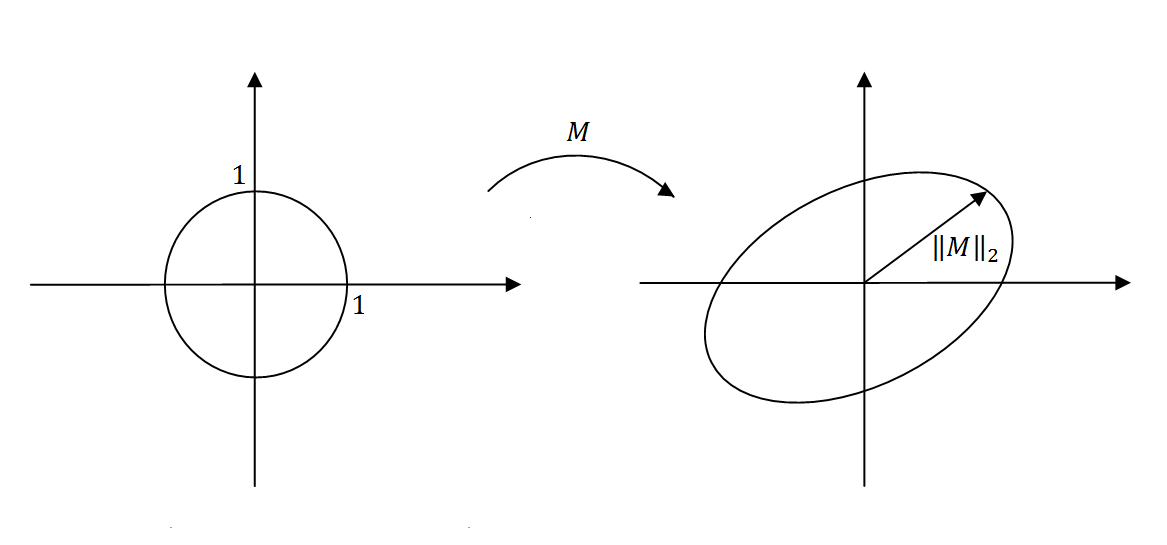
\includegraphics[scale=0.6]{l7_1.png}\end{center}
\textbf{Теорема.}\\
Пусть $||\cdot ||_{\star}$ индуцирована $|\cdot |_{\star}$, тогда \begin{enumerate}
    \item $||\cdot ||$ --- матричная норма, выполнены свойства 0, 1
    \item $||\cdot ||_{\star}$ согласована с $|\cdot |_{\star}$\\
    $\blacktriangleright |Mx|_{\star}\underset{x\neq \bar 0}{=}\cfrac{|Mx|_{\star}}{|x|_{\star}}|x|_{\star} \leqslant \underset{z}{max}\cfrac{|Mz|_{\star}}{|z|_{\star}}|x|_{\star}=||M||_{\star}|x|_{\star}~~\blacksquare$
    \item $||\cdot ||_{\star}$ сохраняет единицу\\
    $\blacktriangleright ||E||_{\star}=\underset{|y|_{\star}=1}{max}|Ey|_{\star}=\underset{|y|_{\star}=1}{max}|y|_{\star}=1~~\blacksquare$ 
    \item Если существует другая норма $||\cdot ||$, согласованная с $||\cdot||_{\star}$, то $||M|| \geqslant ||M||_{\star}$ ($||M_{\star}||$ минимальна).\\
    $\blacktriangleright$ Пусть $|y|_{\star}=1$ и $||M||_{\star}=|My|_{\star}$, тогда длина матрицы $||M||_{\star}=|My|_{\star} \leqslant ||M||\cdot |y|_{\star}=||M||~~\blacksquare$
\end{enumerate}
\textbf{Теорема.}
\begin{center}
  \begin{tabular}{ | c || c |}
    \hline
     Векторная норма $|\cdot|_{\star}$ & Индуцированная норма $||\cdot||_{\star}$\\ \hline \hline
     $||\bar x||_1 = \sum\limits_{i=1}^n |x_i|$ & $||M||_1 = \underset{j}{max}|M^j|_1=\underset{j}{max}\sum\limits_i|m_{ij}|=||M^*||_1$  \\ \hline \hline
     $||\bar x||_2  = \sqrt{\sum\limits_{i=1}^n |x_i|^2}$ & $\sigma(M)=\sqrt{max \lambda_{M^*M}}$ (сингулярный радиус матрицы) \\
    \hline \hline
    $||\bar x||_\infty = \underset{1\leq i \leq n}{max} |x_i|$ & $||M||_{\infty} = \underset{i}{max}|M_i|_1=\underset{i}{max}\sum\limits_j|m_{ij}|$ \\ \hline
  \end{tabular}
\end{center}
Докажем, что векторной норме $|\bar x|_1$ соответствует индуцированная матричная норма $||M||_1$.\\
$\blacktriangleright$ \begin{center} $M=(M^1,\cdots, M^n)$\\
$Mx+M^1x_1+\cdots M^nx_n$\\
$|Mx|_1\leqslant |M^1x_1+\cdots+M^nx_n|_1\leqslant|x_1|~|M^1|_1+\cdots+|M^n|_1~|x_n|\leqslant(|x_1|+\cdots+|x_n|)\underset{j}{max}|M^j|_1\leqslant|\bar x|_1\underset{j}{max}|M^j|_1$\end{center}
Пусть максимум достигается на первом столбце, тогда $|Mx|_1=\sum\limits_{j=1}^n|m_{1j}|=||M||_1$.\\
Оценка достигается, значит это и есть максимум.$~~\blacksquare$\\ \\
\textbf{Домашнее задание 7}\begin{enumerate}
    \item Доказать, что векторной норме $|\bar x|_2$ соответствует индуцированная матричная норма $\sigma(M)$.
    \item Доказать, что векторной норме $|\bar x|_{\infty}$ соответствует индуцированная матричная норма $||M||_{\infty}$.
    \item Является ли матричной нормой $f(A)=\underset{1\leqslant i,~j\leqslant n}{max}|a_{ij}|$ ?
    \item Доказать $||A^{-1}||\geqslant\cfrac{||E||}{||A||}.$
    \item Найти все нормы: $||A||_{\infty}, ~||A||_1, ~\sigma(A)$ для матрицы \[\begin{pmatrix}
1 & 2 & 3\\
4 & 5 & 6\\
7 & 8 & 9
\end{pmatrix}\]
    \item Найти $x,~y,~z,~t$ для матрицы $A$ \[A=\begin{pmatrix}
1 & 2\\
3 & 4
\end{pmatrix}\]
\begin{center}
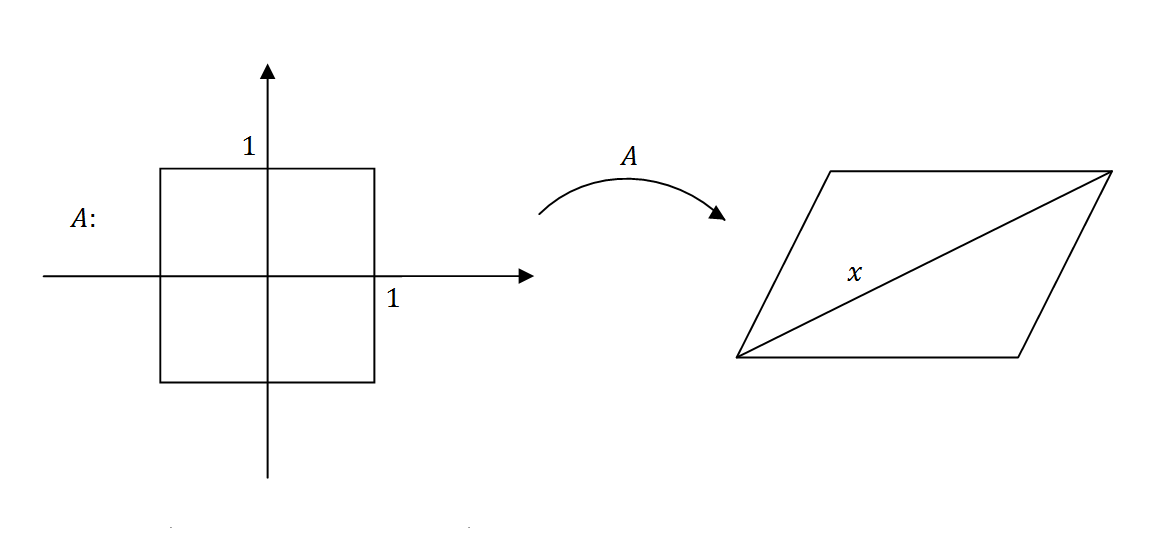
\includegraphics[scale=0.6]{l7_2.png}\\
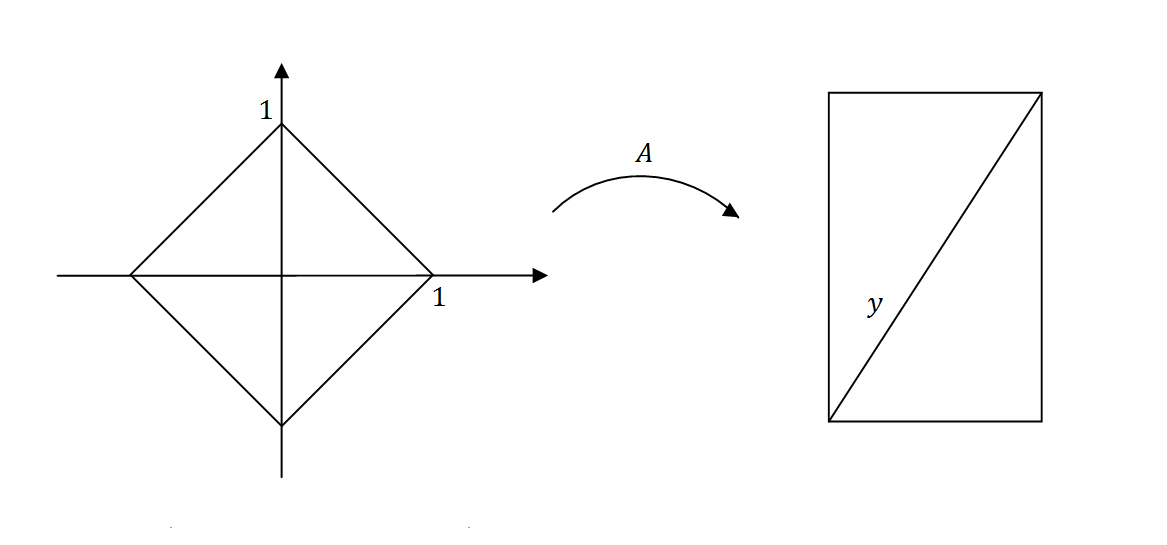
\includegraphics[scale=0.6]{l7_3.png}\\
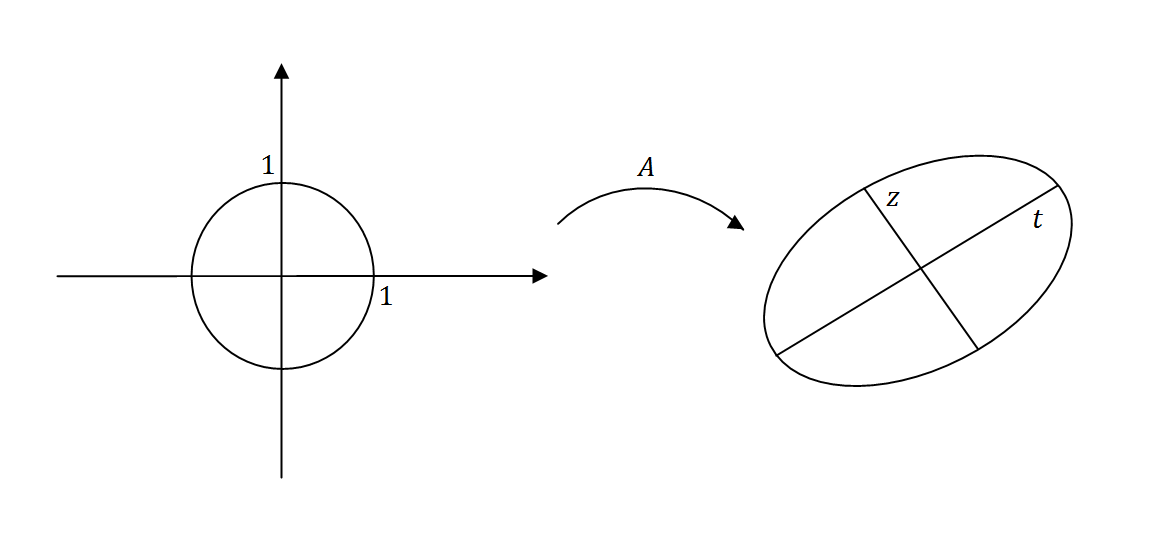
\includegraphics[scale=0.6]{l7_4.png}
\end{center}
\end{enumerate}

\section *{Лекция 8}
\noindent Повторим несколько утверждений из предыдущих лекций.\\
В каждом векторном пространстве $V(\mathbb{R},~\mathbb{C})$ есть норма $\nu(\bar x)\geqslant 0$ такая, что:\begin{enumerate}
\item $\nu(\bar x) > 0$, $\bar x \neq \bar 0$, $\nu(\bar 0) = \bar 0$
\item $\nu(\alpha \bar x) = |\alpha|\nu(\bar x)$
\item $\nu(\bar x + \bar y) \leq \nu(\bar x) + \nu(\bar y)$ для $\forall x, y \in V, \forall \alpha$
\end{enumerate}
Норма Гёльдера: \begin{center}
$|\bar x|_1=|x_1|+\cdots +|x_n|$\\
$|\bar x|_2=\sqrt{|x_1|^2+\cdots +|x_n|^2}$\\
$|\bar x|_{\infty}=\underset{i=1,\cdots,n}{max}|x_i|$ \end{center}
В конечномерном пространстве все нормы эквивалентны.\\
\\
Свойства матричной нормы $M\in M_n$: 
\begin{enumerate}
    \item $||AB||\leqslant ||A||\cdot ||B||$
    \item Матричная норма $||\cdot||$ на $M_n$ согласована с векторной нормой $|\cdot|$ на $\mathbb{C}^n$, если $$|Ax|\leqslant ||A||\cdot |x|$$
    \item Матричная норма сохраняет единицу, если $||E||=1$.
\end{enumerate}
Норма Фробениуса: $||A||_F=\sqrt{\sum\limits_{i,j}|a_{ij}|^2}$.\\
Она удовлетворяет свойствам 1, 2 для $|\cdot|_{1,~2,~\infty}$, но не удовлетворяет свойству 3.\\
\\
$||\cdot||_{\star}$ --- индуцированная матричная норма, если верно $$||A||_{\star}=\underset{\bar x \neq \bar 0}{max} \cfrac{|Ax|_{\star}}{|x|_{\star}}=\bigg( y=\cfrac{\bar x}{|\bar x|_{\star}} \bigg)=\underset{|y|_{\star}=1}{max}|Ay|_{\star}$$
\\
\textbf{Пример 1.}\\
Найти $y$ для матрицы $A$ \[A=\begin{pmatrix}
1 & 2\\
3 & 4
\end{pmatrix}\]
\begin{center}
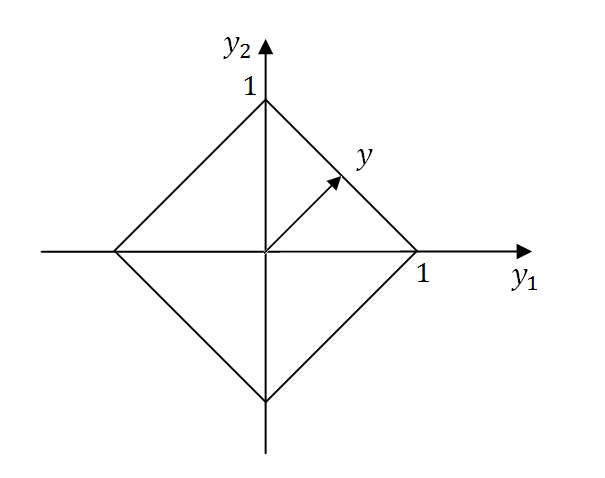
\includegraphics[scale=0.6]{l8_1.png}\end{center}
\[y=\begin{pmatrix}
y_1\\
y_2
\end{pmatrix}\]
$$||A||_1=max|A \bar y|=\underset{|y_1|+|y_2|=1}{max}|y_1+2y_2|+|3y_1+4y_2|$$
Максимум получим при $y_1=0$ и $y_2=1$: $||A||_1=2+4=6$.
\[y=\begin{pmatrix}
0\\
1
\end{pmatrix}\]
~\\ \\
Сингулярное разложение матрицы (SVD): $$A=V\Sigma U^*$$
$V, ~U$ --- унитарные матрицы ($U^*=U^{-1}$)
\[\Sigma=\begin{pmatrix}
\sigma_1 & \cdots & 0\\
\vdots & \ddots & \vdots\\
0 & \cdots & \sigma_n
\end{pmatrix}\]
Тогда $$(A^*A)^*=A^*A=U\Sigma V^* V \Sigma U^*=U\Sigma^2 U^*$$
\[\Sigma^2=\begin{pmatrix}
\sigma_1^2 & \cdots & 0\\
\vdots & \ddots & \vdots\\
0 & \cdots & \sigma_n^2
\end{pmatrix}\]
$\sigma_1 \geqslant \sigma_2 \geqslant \cdots \geqslant \sigma_n \geqslant 0$ --- сингулярные значения матрицы.\\
Аналогично $$AA^*=V\Sigma^2 V^*$$
Здесь $U^1,\cdots,U^n$ --- ортонормированный базис из собственных векторов матрицы $A^*A$, а $V^1,\cdots,V^n$ --- ортонормированный базис из собственных векторов матрицы $AA^*$. $U^i$ и $V^i$ --- правые и левые сингулярные векторы соответственно.\\ \\
$||A||_2=\sigma(A)$\\
$\blacktriangleright$ $$||A||_2=\underset{|x|_2=1}{max}|Ax|_2=\underset{|x|_2=1}{max} \sqrt{(Ax, Ax)}=\underset{|x|_2=1}{max}\sqrt{(Ax)^*Ax}=\underset{|x|_2=1}{max}\sqrt{x^*A^*Ax}$$
$$A^*A\overset{\alpha\to U}{\rightarrow}\Sigma^2$$
$$x=\sum\limits_i \alpha_i U_i,~\sum\limits_i|\alpha_i|^2=1$$
$$xx^*=\sum\limits_i \alpha_i U_i U_i^* \alpha_i=\sum\limits_i \alpha_i U_i U_i^{-1} \alpha_i=\sum\limits_i|\alpha_i|^2$$
\begin{center}
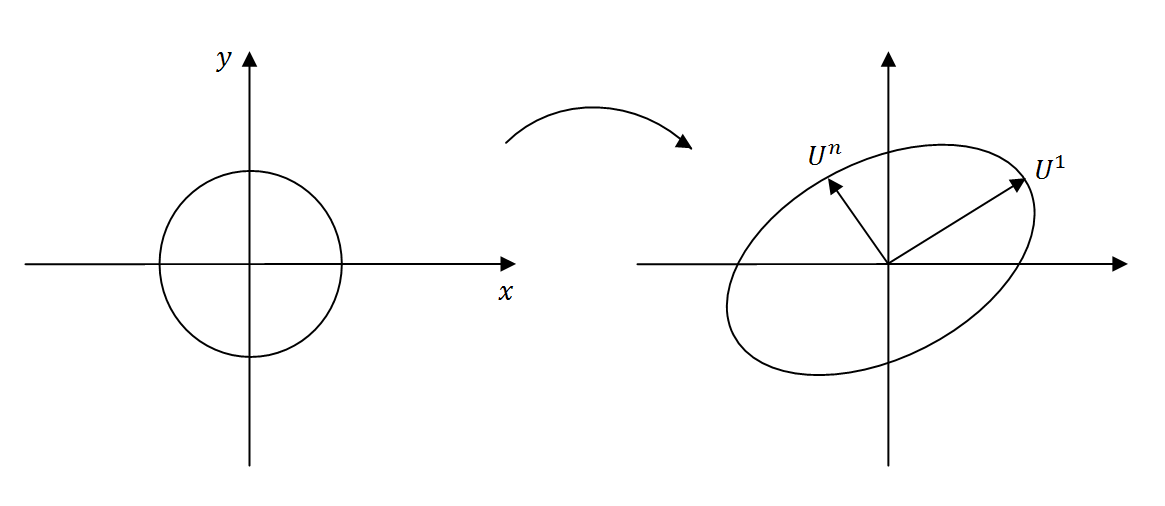
\includegraphics[scale=0.6]{l8_2.png}\end{center}
Подставим в $||A||_2$:\begin{center}
$||A||_2=\underset{|x|_2=1}{max}\sqrt{x^*A^*Ax}=$(в базисе $U$)$=\underset{|x|_2=1}{max}\sqrt{x\Sigma^2 x^*}=\underset{\alpha:~\sum\limits_i |\alpha_i|^2=1}{max}\sqrt{\sum\limits_i \sigma_i^2 |\alpha_i|^2}=\underset{\alpha:~\sum\limits_i |\alpha_i|^2=1}{max}\sqrt{\sigma_1^2|\alpha_1|^2+\cdots+\sigma_n^2|\alpha_n|^2} \leqslant \underset{\alpha:~\sum\limits_i |\alpha_i|^2=1}{max} \sqrt{\sigma_1^2(|\alpha_1|^2+\cdots+|\alpha_n|^2)}=\sigma_1~~\blacksquare$\end{center}
~\\ \\Норма Фробениуса: $$||A||_F=\sqrt{\sum\limits_{i,j}|a_{ij}|^2}=\sqrt{tr(A^*A)}$$
\[A^*A=\begin{pmatrix}
\bar a_{11} & \cdots & \bar a_{n1}\\
* & * & *\\
* & * & *
\end{pmatrix} \cdot \begin{pmatrix}
a_{11} & * & *\\
\vdots & * & *\\
a_{n1} & * & *
\end{pmatrix} = \begin{pmatrix}
\bar a_{11} a_{11}+\cdots+\bar a_{n1} a_{n1} & * & *\\
* & * & *\\
* & * & *
\end{pmatrix}=\] \[=\begin{pmatrix}
|a_{11}|^2+\cdots +|a_{n1}|^2 & * & *\\
* & * & *\\
* & * & *
\end{pmatrix}\]
Получим $\sqrt{tr(A^*A)}=\sqrt{\sigma_1^2+\sigma_2^2+\cdots+\sigma_n^2}$.
\[A=\begin{pmatrix}
1 & 2\\
0 & 3\\
\end{pmatrix}\]
$||A||=1$ ?\begin{center}
$||A||_F=\sqrt{1^2+2^2+3^2}=\sqrt{14}$\\
$||A||_F \geqslant ||A||_2 \geqslant \cfrac{1}{\sqrt{n}}||A||_F=\sqrt{7}$\\
$||A||_1=\underset{j}{max}\sum\limits_i|a_{ij}|=max\{1,~5\}=5$\\
$||A||_{\infty}=\underset{i}{max}\sum\limits_j|a_{ij}|=max\{3,~3\}=3$\end{center}
\textbf{Спектральный радиус} $\rho(A)=|\lambda_{max}(A)|=\underset{i}{max}|\lambda_i|$\\
\\
\textbf{Теорема.} Если матричная норма $||\cdot||$ согласована с некоторой векторной нормой, то $$||A|| \geqslant \rho(A)$$
$\blacktriangleright Av=\lambda v,~v\neq 0$ --- для собственного значения существует собственный вектор.\\
Из определения согласованности векторной нормы: $|Av|\leqslant ||A||\cdot|v|$.
С другой стороны, $|Av|=|\lambda v|=|\lambda||v|$. Получим, что $|\lambda|\leqslant ||A||$, то есть, норма не меньше, чем $\lambda.~~\blacksquare$\\
\\
\textbf{Следствие.} В частности $$\sigma(A)\geqslant \rho(A)$$
\begin{center}
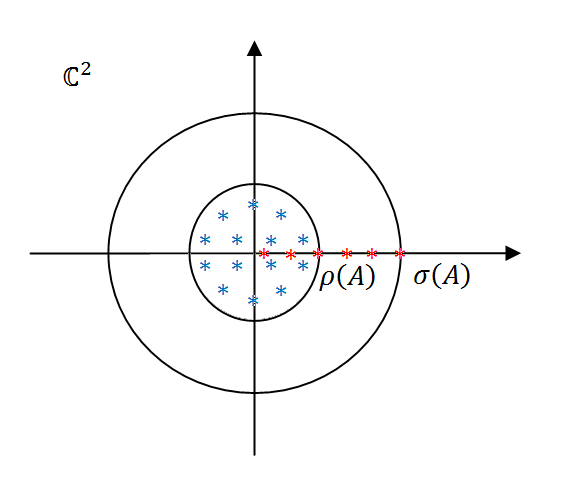
\includegraphics[scale=0.6]{l8_3.png}\end{center}
Здесь $\sigma_i(A)$ --- сингулярные собственные значения, а $\rho(A)~(\lambda_i(A))$ --- собственные значения.\\ \\
\textbf{Утверждение.} Для любой матрицы $A$ и $\forall~ \varepsilon>0$ существует матричная норма $||\cdot ||$, согласованная с некоторой векторной нормой $|\cdot|$, и такая, что $$||A||\leqslant \rho(A) + \varepsilon$$
С помощью $\varepsilon$ можно добиться равенства.\\
\\
Разложение матрицы $A_{n \times n}=A_{n \times r} \cdot A_{r \times
n}$, $A$ ранга $r$.\\
\textbf{Как получить приближенное разложение матрицы?}\\
$A\approx X$, $X$ ранга $r$, $X$ --- ?\\
\textbf{Задача:} найти $X$ ранга $\leqslant r$ такое, что $$||X-A||\to min$$\\
\textbf{Ответ:} для матричных норм $||\cdot||_2,~||\cdot||_F$ (и любой ортогонально инвариантной) $$A=V\Sigma U^*$$
\[\Sigma=\begin{pmatrix}
\sigma_1 & \cdots & 0\\
\vdots & \ddots & \vdots\\
0 & \cdots & \sigma_n
\end{pmatrix}\]
\[\Sigma_r=\begin{pmatrix}
\sigma_1 & \cdots & 0  & \cdots & 0\\
\vdots & \ddots & \vdots & \vdots & \vdots\\
0 & \cdots & \sigma_r &  \vdots & \vdots\\
\vdots & \cdots & \cdots & \ddots & \vdots\\
0 & \cdots & \cdots & \cdots & 0\\
\end{pmatrix}\]
$$X=A_r=V\Sigma_r U^*$$
Для $||A||=||A||_2=\sigma(A)$. \\
$\blacktriangleright U^1,\cdots, U^n$ --- правый сингулярный базис.
Пусть $\bar w \in <U^1,\cdots,U^{r+1}> \cap~ Ker X$, где $Ker X \geqslant n-r$, а $X$ ранга $\leqslant r$, $|w|=1$.\\
Так как $|Mx|\leqslant ||M||,~|x|=1$, тогда \begin{center}
$(||X-A||_2)^2 \geqslant(|(X-A)w|_2)^2=|Xw-Aw|^2=|Aw|^2=$ (в базисе $U$) =
\end{center}
\[=\Bigg| V\begin{pmatrix}
\sigma_1 & \cdots & 0  & \cdots & 0\\
\vdots & \ddots & \vdots & \vdots & \vdots\\
0 & \cdots & \sigma_{r+1} &  \vdots & \vdots\\
\vdots & \cdots & \cdots & \ddots & \vdots\\
0 & \cdots & \cdots & \cdots & 0\\
\end{pmatrix} \begin{pmatrix}
w_1\\
\vdots\\
w_{r+1}\\
\vdots\\
0\\
\end{pmatrix}\Bigg|^2 =\Bigg|V \begin{pmatrix}
\sigma_1 w_1\\
\vdots\\
\sigma_{r+1} w_{r+1}\\
\vdots\\
0\\
\end{pmatrix} \Bigg|^2 =\Bigg| \begin{pmatrix}
\sigma_1 w_1\\
\vdots\\
\sigma_{r+1} w_{r+1}\\
\vdots\\
0\\
\end{pmatrix} \Bigg|^2=\]$$=\sigma_1^2|w_1|^2+\cdots+\sigma_{r+1}^2|w_{r+1}|^2 \geqslant \sigma_{r+1}^2(|w_1|^2+\cdots+|w_{r+1}|^2)=\sigma_{r+1}^2|w|=\sigma_{r+1}^2$$ для любой матрицы $X$, где 
\[||A_r-A||_2=||V(\Sigma-\Sigma_r)U^*||_2=||\Sigma-\Sigma_r||_2 = \Bigg| \Bigg|\begin{pmatrix}
0 & \cdots & 0  & \cdots & 0\\
\vdots & \ddots & \vdots & \vdots & \vdots\\
0 & \cdots & \sigma_{r+1} &  \vdots & \vdots\\
\vdots & \cdots & \cdots & \ddots & \vdots\\
0 & \cdots & \cdots & \cdots & \sigma_n\\
\end{pmatrix}\Bigg|\Bigg|_2=\sigma_{r+1}\]
Достигается для $r$, значит она оптимальна (меньше нет). Для евклидовой нормы это лучшее приближение. $\blacksquare$\\ \\
\textbf{Пример 2.}\\
Найти наилучшее приближение $A_1$ ранга 1 для матрицы $A$ в норме $||\cdot||_2$ и найти $||A-A_1||_2$, где
\[A = \begin{pmatrix}
6 & 0 & 6\\
0 & 12 & 6\\
6 & 6 & 9
\end{pmatrix}\]
Так как матрица $A$ симметричная, можно не находить $A^*A$. Найдем сразу собственное значение и собственный вектор.
\begin{center}
$det(A-\lambda E)=0$\\
$\lambda_1=18,~\lambda_2=9,~\lambda_3=0$\end{center}
\[\Sigma = \begin{pmatrix}
18 & 0 & 0\\
0 & 9 & 0\\
0 & 0 & 0
\end{pmatrix}\]
Хотим построить сингулярное разложение $A=V\Sigma U^*$. Если $A^*=A$, то $V=U$.\\
После решения СЛАУ $(A-\lambda_i E)x=0$ из $\lambda_i$ получим $v_i$.
\[V=U= \begin{pmatrix} [r]
\cfrac{1}{3} & \cfrac{2}{3} & -\cfrac{2}{3}\\
\cfrac{2}{3} & -\cfrac{2}{3} & -\cfrac{1}{3}\\
\cfrac{2}{3} & \cfrac{1}{3} & \cfrac{2}{3}
\end{pmatrix}\]
\[\Sigma_1 = \begin{pmatrix}
18 & 0 & 0\\
0 & 0 & 0\\
0 & 0 & 0
\end{pmatrix}\]
\[X=A_1 = V\Sigma_r U^*=\begin{pmatrix}
2 & 4 & 4\\
4 & 8 & 8\\
4 & 8 & 8
\end{pmatrix}\]
Ранг матрицы $A_1$ равен $1$, $||A-A_1||_2=9$ (наибольший из остальных $\sigma$).\\ \\
\noindent \textbf{Домашнее задание 8}

\begin{enumerate}
\item
Найти наилучшее приближение ранга 2 по фробениусовой норме для матрицы 
\[B = \begin{pmatrix}
6 & 0 & 6\\
0 & 12 & 6\\
6 & 6 & 9
\end{pmatrix}\]

    \item Найти наилучшее приближение $B_1$ ранга 1 для матрицы $B$ в норме $||\cdot||_2$ и найти $||B-B_1||_2$, где
\[B = \begin{pmatrix}
6 & 30 & -21\\
17 & 10 & -22\\
\end{pmatrix}\]

    \item Доказать утверждение из лекции: для любой матрицы $A$ и $\forall~ \varepsilon>0$ существует матричная норма $||\cdot ||$, согласованная с некоторой векторной нормой $|\cdot|$ и такая, что $$||A||\leqslant \rho(A) + \varepsilon .$$
\end{enumerate}

\section *{Лекция 9}
\noindent\textbf{Оценка собственных значений}\\ \\
\textbf{Оценка:} Если $||A||$ --- матричная норма, согласованная с некоторой векторной нормой, то $$|\lambda|\leqslant||A||,$$ где $\lambda$ --- любое собственное значение матрицы $A$.\\
\\
То же можно применить и к обратной матрице.\\
\\
\textbf{Утверждение.} Если матрица $A$ --- невырожденная, то для любого собственного значения $\lambda$ верно $$\cfrac{1}{||A^{-1}||}\leqslant|\lambda|\leqslant||A||$$
~\\Все собственные значения матрицы $A$ находятся между двумя кольцами.
\begin{center}
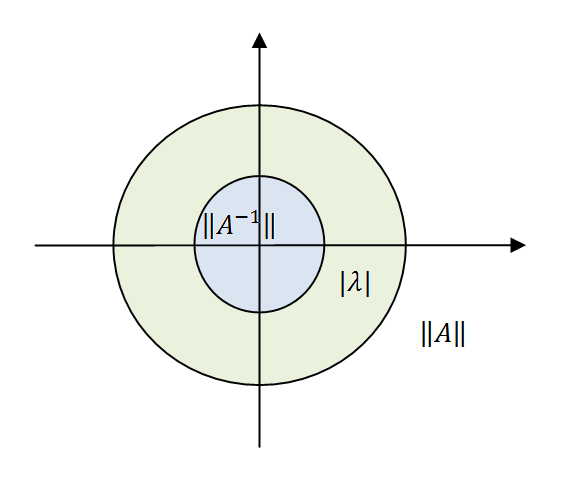
\includegraphics[scale=0.8]{l9_1.png}
\end{center}
$\blacktriangleright$ Пусть $\lambda$ --- собстенное значение матрицы $A$, то есть, $A\bar x=\lambda\bar x$ для некоторого $\bar x\neq \bar 0$, тогда
\begin{center}
$\bar x=\lambda A^{-1} \bar x$\\
$\lambda^{-1}\bar x=A^{-1}\bar x$
\end{center}
То есть, $\lambda^{-1}$ --- собственное значение для матрицы $A^{-1}$.\\
\begin{center}
$|\lambda^{-1}|\leqslant||A^{-1}||$ (из оценки)\\~\\
$|\lambda|^{-1}\leqslant ||A^{-1}||$\\
$|\lambda|\geqslant \cfrac{1}{||A^{-1}||}$
\end{center}
С учетом оценки, получим $$\cfrac{1}{||A^{-1}||}\leqslant|\lambda|\leqslant||A||~~\blacksquare$$ 
Матрица называется матрицей \textbf{с диагональным преобладанием}, если каждое из чисел на диагонале больше суммы модулей по строке, то есть, $$\forall i=1,\cdots,n~|a_{ii}|>\sum\limits_{k\neq i}|a_{ik}|.$$
~\\
\textbf{1-я Теорема Гершгорина.} Все собственные значения матрицы $A_{n \times n}=(a_{ij})$ содержатся в объединении кругов на комплексной плоскости. $$|\lambda-a_{ii}|\leqslant \sum\limits_{k=1, k\neq i}^n|a_{ik}|,~i=1,\cdots n.$$
Обозначим: $R_i=\sum\limits_{k=1, k\neq i}^n|a_{ik}|.$\\
Каждое из собственных значений $\lambda$ матрицы $A$ всегда расположено в одном из кругов.
\begin{center}
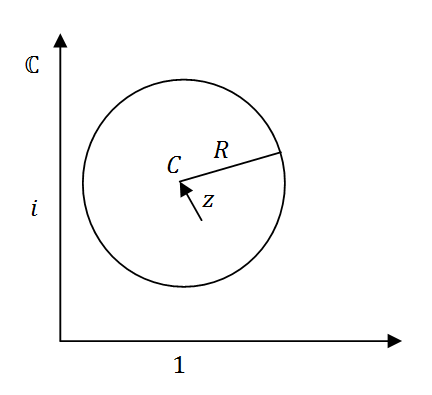
\includegraphics[scale=0.8]{l9_2.png}
\end{center}
$$|z-C|\leqslant R$$
\[\begin{pmatrix}
* & \cdots & \cdots & \cdots & \cdots\\
a_{i1} & \cdots & a_{ii} & \cdots & a_{in}\\
\cdots & \cdots & \cdots & \cdots & *\\
\end{pmatrix}\]
Круг с центром в точке $C=a_{ii}$ и радиусом $R=R_i=\sum\limits_{k\neq i}|a_{ik}|.$\\
\\
Если $\lambda$ --- собственное значение матрицы $A$, то
$$|A-\lambda E|=|(A-\lambda E)^T|=|A^T-\lambda E|=0$$
Получили, что $\lambda$ --- собственное значение матрицы $A^T$.\\ 
У матрицы $A^T$ собственные значения те же, что и у матрицы $A$, а строки $A^T$ --- столбцы $A$, такие что:\\
\textbf{Следствие.} Все собственные значения матрицы $A$ содержатся в объединении кругов на комплексной плоскости. $$|\lambda-a_{ii}|\leqslant \sum\limits_{k=1, k\neq i}^n|a_{ki}|,~i=1,\cdots n.$$
Обозначим: $C_i=\sum\limits_{k=1, k\neq i}^n|a_{ki}|.$\\
\textbf{Доказательство теремы.}\\
$\blacktriangleright$ Пусть $\lambda$ --- собственное значение $A$, докажем, что $\lambda$ находится в объединении кругов Гершгорина.\\
У каждого собственного значения существует собственный вектор: $$Ax=\lambda x, \bar x\neq \bar 0.$$
Пусть, например, $|x_1|$ --- наибольший из модулей $|x_i|$, то есть, $|x_1|\geqslant|x_2|,|x_3|,\cdots,|x_n|$. Тогда из $Ax=\lambda x$ следует
\begin{center}
$a_{11}x_1+\cdots+a_{1n}x_n=\lambda x_1$\\
$(\lambda-a_{11})x_1=a_{12}x_2+\cdots+a_{1n}x_n$\\
$|\lambda-a_{11}||x_1|=|a_{12}|x_2+\cdots+a_{1n}x_n|\leqslant\sum\limits_{k=2}^n|a_{1k}||x_k|\leqslant\sum\limits_{k=2}^n|a_{1k}||x_1|=|x_1|R_1$\\
$|\lambda-a_{11}|\leqslant R_1=\sum\limits_{k=2}^n|a_{1k}|$
\end{center}
Получили, что если $x_1$ --- наибольший, то собственное значение попадает в первый круг Гершгорина. И так далее, если $x_n$ --- наибольший, то собственное значение попадет в $n$-ый круг Гершгорина.$~~\blacksquare$\\ \\
\textbf{Следствие.} Матрица с диагональным преобладанием является невырожденной.\\
$\blacktriangleright$ Доказательство следует из того, что в такой матрице все собственные значения $\lambda\neq 0~~\blacksquare$\\ \\
\textbf{Пример 1.}\\
Дана матрица $n\times n$:
\[A=\begin{pmatrix}[r]
2 & -1 & \cdots & \cdots & \cdots & \cdots\\
-1 & 2 & -1 & \cdots & \cdots & \cdots\\
\cdots & -1 & 2 & -1 & \cdots & \cdots\\
\cdots & \cdots & \cdots & \ddots & \cdots & \cdots\\
\cdots & \cdots & \cdots & -1 & 2 & -1\\
\cdots & \cdots & \cdots & \cdots & -1 & 2\\
\end{pmatrix}\]
Вычислим круги Гершгорина.
\begin{center}
\begin{tabular}{|c|c|c|}
\hline
№ & Центр & Радиус \\ \hline
1 & 2 & |-1|=1 \\ \hline
2~--~(n-1) & 2 & |-1|+|-1|=2 \\ \hline
n & 2 & |-1|=1 \\ \hline
\end{tabular}\\
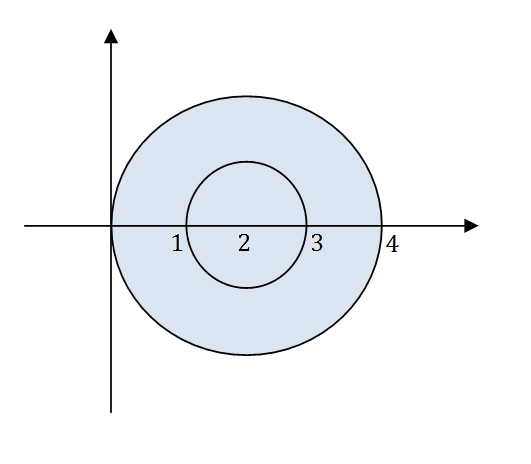
\includegraphics[scale=0.8]{l9_3.png}
\end{center}
Все собственные значения содержатся в объединении кругов на комплексной плоскости.\\
\begin{center}
$|\lambda-2|\leqslant 1$\\
$|\lambda-2|\leqslant 2$
\end{center}
$
\left\{
\begin{array}{lcl}
    A^*=A \\
    A\in M_n(\mathbb{R}) \\
\end{array}
\right.
$\\ \\
Получили, что $\lambda_i\in \mathbb{R},~0\leqslant\lambda_i\leqslant 4$.\\
\\
Если $\chi_A(\lambda)=(\lambda_1-\lambda)^{k_1}\cdots(\lambda_s-\lambda)^{k_s}$, где $\lambda_i$ различны, то числа $k_i$ называют кратностями соответствующих собственных значений.\\ \\
\textbf{2-я Теорема Гершгорина.} Если объединение $U$ $r$ кругов Гершгорина не пересекается с остальными $(n-r)$ кругами, то $U$ содержит ровно $r$ собственных значений с учетом кратностей.\\
$\blacktriangleright$ Пусть $D$ --- диагональная часть матрицы $A$
\[D=\begin{pmatrix}
a_{11} & \cdots & 0 \\
\vdots & \ddots & \vdots \\
0 & \cdots & a_{nn} \\
\end{pmatrix}\]
а матрица $B=A-D$ --- матрица $A$ без диагональных элементов 
\[B=\begin{pmatrix}
0 & a_{12} & \cdots \\
a_{21} & \ddots & \cdots \\
\cdots & \cdots & 0 \\
\end{pmatrix}\]
Рассмотрим непрерывное непрерывное семейство матриц $$A_t=D+tB$$
Это непрерывная функция из $\mathbb{R}$ в $M_n(\mathbb{C})$. Здесь $A_0=D,~A_1=A$.\\
Корни характеристического многочлена матрицы $A_t$ непрерывно зависят от $t_0$. При $t=0$ --- это $\lambda_1(0)=a_{11},\cdots,\lambda_n(0)=a_{nn}$, а при $t=1$ --- это собственные числа матрицы $A$.\\
По первой теореме Гершгорина $\forall t~\lambda\in U$ в объединении кругов Гершгорина с центрами $a_{11},\cdots,a_{nn}$ и радиусами $$R_i(t)=tR_i.$$
С ростом $t$ круги "раздуваются" из точек (движение по непрервной кривой).
\begin{center}
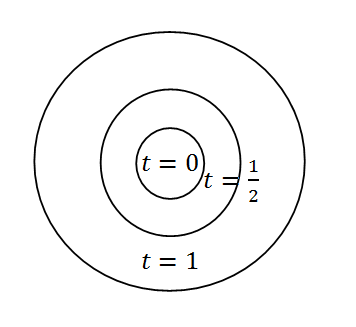
\includegraphics[scale=0.8]{l9_4.png}
\end{center}
Если объединение некоторых $r$ кругов Гершгорина не пересекаются с остальными при $t=1$, то и при $t<1$ тоже, значит каждое из соответствующих $r$ собственных значений $\lambda_i$ двигается из $a_{ii}$ по непрерывной кривой внутри $U.~~\blacksquare$\\
\\
\textbf{Пример 2.}\\
Пусть 
\[A=\begin{pmatrix}[r]
-1 & 1 \\
-4 & -5 \\
\end{pmatrix}\]
\[\chi_A(\lambda)=|A-\lambda E|=\begin{vmatrix}[r]
-1-\lambda & 1 \\
-4 & -5-\lambda \\
\end{vmatrix}=(\lambda +3)^2\]
Получили, что $\lambda_1=\lambda_2=-3$.
\begin{center}
\includegraphics[scale=0.8]{l9_5.png}
\end{center}
\[A=\begin{pmatrix}[r]
-1 & t \\
-4t & -5 \\
\end{pmatrix}=\begin{pmatrix}[r]
-1 & 0 \\
0 & -5 \\
\end{pmatrix}+ t\begin{pmatrix}[r]
0 & 1 \\
-4 & 0 \\
\end{pmatrix}\]
Характеристический многочлен $$\chi_{A_t}(\lambda)=|A_t-\lambda E|=\lambda^2+6\lambda+5+4t^2$$
\begin{center}
$\lambda_{1,2}=-3\pm 2\sqrt{1-t^2},~t<1$\\
$\lambda_{1,2}=-3\pm i\cdot 2\sqrt{1-t^2},~t>1$
\end{center}
\textbf{Пример 3.}\\
\[A=\begin{pmatrix}
5 & 1 & 0 \\
0 & 1 & 2 \\
0 & 2 & 1 \\
\end{pmatrix}\]
Для матрицы $A$:
\begin{center}
$|\lambda-5|\leqslant 1$\\
$|\lambda-1|\leqslant 2$ --- 2 раза
\end{center}
\begin{center}
\includegraphics[scale=0.8]{l9_6.png}
\end{center}
В $K_1$ находится одно собственное значение $\lambda_1$, в $K_2$ --- два $\lambda_2,~\lambda_3$.\\
Для матрицы $A^T$
\[A^T=\begin{pmatrix}
5 & 0 & 0 \\
1 & 1 & 2 \\
0 & 2 & 1 \\
\end{pmatrix}\]
\begin{center}
$K_1':~|\lambda-5|=0 \Rightarrow \lambda_1'=5$\\
$K_2':~|\lambda-1|\leqslant 3$\\
$K_3':~|\lambda-1|\leqslant 2$
\end{center}
То есть, $\lambda_2',~\lambda_3'\in K_2'=K_2'\cup K_3'$.\\
Так как $\{\lambda_1,~\lambda_2,~\lambda_3\}=\{\lambda_1',~\lambda_2',~\lambda_3'\}$ --- те же собственные значения, то $\lambda_1=\lambda_1=5$.\\
Значит $\lambda_2'$ и $\lambda_3'$ --- те же, что $\lambda_2$ и $\lambda_3$, то есть, $\lambda_2',~\lambda_3'\in K_2$.\\
Итог для матрицы $A$: $\lambda_1=5$, а $\lambda_2,~\lambda_3$ удовлетворяют условию $|\lambda-1|\leqslant 2$.\\ \\
\textbf{Домашнее задание 9}\begin{enumerate}
\item Нарисовать круги Гершгорина для матрицы $A$ и с их помощью оценить собственные значения. Вычислить собственные значения и сравнить результаты.
\[A = \begin{pmatrix}
5 & 0.3\\
-0.5 & 2\\
\end{pmatrix}\]
\item С помощью теоремы Гершгорина нарисовать область, где находятся собственные значения матрицы $A$.
\[A = \begin{pmatrix}
3 & 0.2 & -0.2\\
0 & 2 & 0.1\\
0.1 & 0.4 & 1\\
\end{pmatrix}\]
\item Доказать, что определитель матрицы $A$ не равен 0 ($detA\neq 0$). Нарисовать наименьшую область, содержащую собственные значения.
\[A = \begin{pmatrix}
2 & cos~x & cos^2~x\\
0 & 5 & sin^2~x\\
3sin^2~x & 3 & 10\\
\end{pmatrix}\]
\item Доказать, что в номерах 1, 2 и 3 все собственные значения --- положительные действительные числа и оценить их.\\
Подсказка: если $\lambda$ --- собственное значение матрицы $A$, то и $\overline \lambda$ --- тоже ее собственное значение, так как $|\overline{A-\lambda E}|=|A-\overline\lambda E|=0$.
\end{enumerate}
~\\
\section *{Лекция 10}
\noindent\textbf{Функции от матрицы.}\\
Пусть $A$ --- квадратная матрица ($A\in M_n(\mathbb{C})$)
$$A^m=A~ \dot~ ... ~\dot~ A,~A^0=E$$
Если $A$ невырожденная, то $$A^{-m}=(A^{-1})^m$$
\textbf{Многочлен от матрицы:} если 
$f(x)=a_0+a_1x+\cdots+a_mx^m$, то
$f(A)=a_0E+a_1A+\cdots +a_mA^m$ --- тоже матрица.\\
\\
\textbf{Пример 1.}\\
\[A = \begin{pmatrix}
0 & 1\\
1 & 0\\
\end{pmatrix}\]
$f(x)=x^2-1$\\
Тогда 
\[f(A)=A^2-1\cdot E = \begin{pmatrix}
1 & 0\\
0 & 1\\
\end{pmatrix} - \begin{pmatrix}
1 & 0\\
0 & 1\\
\end{pmatrix} = \begin{pmatrix}
0 & 0\\
0 & 0\\
\end{pmatrix} =0\]
\textbf{Утверждение.} Если $C$ --- невырожденная матрица (например, $C=Te \to e'$ --- матрица перехода от базиса $e$ к базису $e'$ в $\mathbb{C}^n$) и $A'=C^{-1}AC$ (то есть, $A'$ --- матрица того же линейного оператора, что и $A$, в новом базисе $e'$ вместо старого $e$), то для любого многочлена $f(x)$ верно $f(A')=C^{-1}f(A)C$.\\
$\blacktriangleright$ Если $f(x)=\sum\limits_{i=0}^n a_iA^i$, то $f(A')=\sum\limits_{i=0}^n a_i A'^i=\sum\limits_{i=0}^n a_iC^{-1}AC\cdot C^{-1}AC\cdot C^{-1}\cdots AC=\\=\sum\limits_{i=0}^n a_i C^{-1}A^iC=C^{-1}(\sum\limits_{i=0}^na_iA^i)C=C^{-1}f(A)C~~\blacksquare$\\
\\
\textbf{Следствие.} $$f(A)=0 \Leftrightarrow f(A')=0$$
\\
Если $A'$ --- диагональная матрица\[A'=\begin{pmatrix}
d_1 & \cdots & 0\\
\vdots & \ddots & \vdots\\
0 & \cdots & d_n
\end{pmatrix},\]
то \[f(A')=\sum\limits_{i=0}^n a_i(A')^i=\sum\limits_{i=0}^n a_i\begin{pmatrix}
d_1^i & \cdots & 0\\
\vdots & \ddots & \vdots\\
0 & \cdots & d_n^i
\end{pmatrix}=\begin{pmatrix}
f(d_1) & \cdots & 0\\
\vdots & \ddots & \vdots\\
0 & \cdots & f(d_n)
\end{pmatrix}\]
В частности, если все собственные значения $\lambda_1,\cdots, \lambda_n$ матрицы $A$ различны, то 
\[A'=C^{-1}AC=\begin{pmatrix}
\lambda_1 & \cdots & 0\\
\vdots & \ddots & \vdots\\
0 & \cdots & \lambda_n
\end{pmatrix},~~C= \begin{pmatrix}
v_1~| & ~v_2~| & ~\cdots~| & ~v_n\\
\end{pmatrix}\]
Причем, $v_1$ --- собственный вектор, соответствующий собственному значению $\lambda_1$ (то есть, $Av_1=\lambda_1 v_1$), $\cdots$, $v_n$ --- собственный вектор, соответствующий собственному значению $\lambda_n$ ($Av_n=\lambda_n v_n$), тогда $A=CA'C^{-1}$
\[f(A)=Cf(A')C^{-1}=C\begin{pmatrix}
f(\lambda_1) & \cdots & 0\\
\vdots & \ddots & \vdots\\
0 & \cdots & f(\lambda_n)
\end{pmatrix}C^{-1}\]
\\
\textbf{Жорданова форма.}\\
\textbf{Жорданова клетка} --- это матрица вида
\[J=J_k(\lambda)=\begin{pmatrix}
\lambda &  1 & \cdots & 0\\
\vdots & \ddots & 1 & \vdots\\
\vdots & 0 & \ddots & 1\\
0 & \cdots & \cdots & \lambda
\end{pmatrix}C^{-1}\]
Например, 
\[J_2(0) = \begin{pmatrix}
0 & 1\\
0 & 0\\
\end{pmatrix}\]
\[J_3(5) = \begin{pmatrix}
5 & 1 & 0\\
0 & 5 & 1\\
0 & 0 & 5\\
\end{pmatrix}\]
Например, если $V=P_n=\mathbb{C}[$x$]_{\leqslant n}=\{a_0+a_1x+\cdots +a_nx^n\},~D:V\to V:~f(x) \mapsto f'(x)$ --- дифференцирование. $f$ --- собственный вектор для $D$ тогда и только тогда, когда $Df=\lambda f$, то есть $f'(x)=\lambda f(x)$, где $\lambda$ --- число, тогда $f(x)=a_0=const,~f'(x)=0\cdot f(x)=0$.\\
\\
\textbf{Базис Маклорена.}\\
$$e_0=1,~e_1=\cfrac{x}{1!},\cdots,~e_u=\cfrac{x^u}{u!}$$
В этом базисе
$$D(e_k)=\bigg(\cfrac{x^k}{k!}\bigg)'=\cfrac{x^{k-1}}{(k-1)!}=e_{k-1}$$
\[D_e = \begin{pmatrix}
0 &  1 & \cdots & 0\\
\vdots & \ddots & 1 & \vdots\\
\vdots & 0 & \ddots & 1\\
0 & \cdots & \cdots & 0
\end{pmatrix} = J_n(0)\]
\[J_n(0)^k = \begin{pmatrix}
0 &  \cdots & \underset{k}{1} & \cdots & 0\\
\vdots & \cdots & \ddots & \underset{k+1}{1} & \vdots\\
\vdots & \cdots & 0 & \ddots & \underset{n}{1}\\
0 & \cdots & \cdots & \cdots & 0
\end{pmatrix}\]
(так как $D^k(e_u)=e_{n-k}$ и т.д.)\\
\\
\textbf{Предложение.} Если $f(x)$ --- многочлен, то
\[f(J_k(\lambda)) = \begin{pmatrix}
f(\lambda) & \cfrac{f'(\lambda)}{1!} & \cdots & \cfrac{f^{(k-1)}(\lambda)}{(k-1)!}\\
0 & \ddots & \cdots & \cfrac{f^{(k-2)}(\lambda)}{(k-2)!}\\
\vdots & 0 & \ddots & \vdots\\
0 & \cdots & 0 & f(\lambda)\\
\end{pmatrix}\]
$\blacktriangleright$ Так как $f(x)=\sum\limits_{i=0}^n a_ix^i$, то достаточно проверить формулу для $f(x)=x^i$. Тогда в каждой клетке получаем $\sum\limits_{i=0}^n a_i\cfrac{(x^i)^{(t)}}{t!}=\cfrac{f^{(t)}(x)}{t!}$ для подходящего $t$. \\
Имеем: при $f(x)=x^i$
\[f(J_k(\lambda))=\begin{pmatrix}
\lambda &  1 & \cdots & 0\\
\vdots & \ddots & 1 & \vdots\\
\vdots & 0 & \ddots & 1\\
0 & \cdots & \cdots & \lambda
\end{pmatrix}^i= \bigg( \lambda \begin{pmatrix}
1 &  0 & \cdots & 0\\
0 & \ddots & 1 & \vdots\\
\vdots & 0 & \ddots & 0\\
0 & \cdots & 0 & 1
\end{pmatrix} + \begin{pmatrix}
0 &  1 & \cdots & 0\\
\vdots & \ddots & 1 & \vdots\\
\vdots & 0 & \ddots & 1\\
0 & \cdots & \cdots & 0
\end{pmatrix} \bigg)^i=\]
$$=(\lambda E+J_k(0))^i=\sum\limits_{t=0}^i\lambda^t J_k(0)^{i-t}C_i^t$$
Ненулевые элементы только в клетках с координатами $(a, a+(i-t))_i$, в этих клетках стоит
$$\lambda^tC_i^t=\cfrac{\lambda^t i!}{t!(i-t)!},$$
при этом
$$f^{(i-t)}(\lambda)=\cfrac{i!}{t!}\lambda^t$$
\\
\textbf{Теорема о Жордановой форме.} Длялюбого линейного оператора $\phi$ в $\mathbb{C}^n$ существует базис (жорданов базис), в котором матрица оператора $\phi$ преобретает вид
\[\phi_i=J(\phi) = \begin{pmatrix}
J_1 & \cdots & 0\\
\vdots & \ddots & \vdots\\
0 & \cdots & J_T\\
\end{pmatrix},\]
где $J_i$ --- жордановы клетки.\\
\\
Если $A$ --- матрица $n\times n$, что
$$\phi_A(\lambda)=det(A-\lambda E)=(\lambda_1 - \lambda)^{k_1}\cdots(\lambda_i - \lambda)^{k_i},$$
то $k_i$ --- кратности собственных значений $\lambda_i$.
\[ 
J(A)=
\left(
\begin{BMAT}[8pt]{c:cc:ccc:c}{c:cc:ccc:c}
  \lambda_1 & 0  &  & & 0 & & 0 \\
  0 & \lambda_2 & 1 &  & 0  & & 0\\
   & 0 & \lambda_2 &  & & &\\
  &  & & \lambda_3 & 1 & 0 & \\
  0& 0 &  & \vdots & \ddots & 1 & 0 \\
  &  &  & 0 & \cdots & \lambda_3 &  \\
  0 & 0 &  &  & 0 & & \ddots
\end{BMAT} 
\right)
\]
\textbf{Следствие.} Если $J=J(A)$ --- жорданова форма $A$, $C$ --- матрица, в которой по столбцам записан жорданов базис, то
$$f(J)=C^{-1}f(A)C \Leftrightarrow f(A)=Cf(J)C^{-1},$$
где 
\[ 
f(J)=
\left(
\begin{BMAT}[8pt]{c:c:c}{c:c:c}
  f(J_1) & \cdots  & 0 \\
  \vdots & f(J_2) & \vdots\\
  0 & \cdots  & \ddots\\
\end{BMAT} 
\right)
\]
\textbf{Аннулирующий многочлен} матрицы $A$ --- такой многочлен $f(x)$, что $f(A)=0$.\\ \\
\textbf{Минимальный многочлен} матрицы $A$ (обозначается $m_A(x)$) --- это аннулирующий многочлен наименьшей возможной степени со старшим коэффициентом 1.\\
\\
\textbf{Пример 2.}\\
$\chi_A(\lambda)$ --- аннулирующий многочлен для $A$ (по теореме Гамильтона-Кели).
$$\chi_A(A)=C^{-1}\chi_A(J)C=C^{-1}((\lambda_1E-J)^{k_1}\cdots(\lambda_iE-J)^{k_i})C =$$  
\[=C^{-1}\left(
\begin{BMAT}[8pt]{ccc:c}{ccc:c}
  0 & 1 & 0  & 0 \\
  \vdots & \ddots & 1 &\vdots\\
  0 & \cdots & 0 & \vdots\\
  0 & \cdots & \cdots & \ddots\\
\end{BMAT} 
\right)
^{k_i}\cdots C = C^{-1}OC\]
Получим $\chi_A(\lambda)=0$.\\
\\
Пусть $m_i$ --- порядок наибольшей жордановой клетки с $\lambda=\lambda_i$ (геометрическая кратность собственного значения). Тогда $m_i\leqslant k_i$ и $m_A(x)=(x-\lambda_1)^{m_1}\cdots (x-\lambda_i)^{m_i}$ --- минимальный многочлен матрицы $A$ (он же --- минимальный многочлен $J$).\\
\\
Как вычислить $f(A)$, зная минимальный многочлен $m_A(x)=(x-\lambda_1)^{m_1}\cdots (x-\lambda_s)^{m_s}$?\\
Если $f(x)=m_A(x)q(x)+R(x)$ --- деление с остатком, где $degR(x)<d$ ($d=deg m_A(x)$ --- степень минимального многочлена), то 
$f(A)=0\cdot q(A)+R(A)=R(A)$ --- \textbf{многочлен Лагранжа-Сильвестра}.\\
\\
$\lambda_1,\cdots,\lambda_s$ --- спектр, $R_1,\cdots,R_s$ --- соответствующие алгебраические кратности.\\
\[
\begin{BMAT}[8pt]{ccc}{ccc}
  f(\lambda_1) & \cdots & f(\lambda_s) \\
  \vdots & \ddots &\vdots\\
  f^{(k_1-1)}(\lambda_1) & \cdots & f^{(k_s-1)}(\lambda_s)\\
\end{BMAT} 
\]
$$k_1+\cdots +k_s=u$$
$P$ --- многочлен Лагранжа-Сильвестра.
$$P(\lambda_j)=f(\lambda_k)$$
$$ \vdots$$
$$P^{(k_j-1)}(\lambda_j)=f^{(k_j-1)}(\lambda_j),~j=1,\cdots, s$$
Определяющий многочлен
$$\psi(\lambda)=(\lambda-\lambda_1)^{k_1}\cdots(\lambda-\lambda_s)^{k_s}$$
многочлены
$$\phi_j=\cfrac{\psi(\lambda)}{(\lambda-\lambda_j)^{k_j}}$$
Тогда искомый многочлен
$$P(\lambda)=\sum\limits_{j=1}^s(\alpha_{j1}+\alpha_{j2}(\lambda-\lambda_j)+\cdots +\alpha_{jk_j}(\lambda-\lambda_j)^{k_j-1})\psi_j(\lambda)$$
$$\alpha_{jl}=\cfrac{1}{(l-1)!}\bigg(\cfrac{f(\lambda)}{\psi_j(\lambda)}\bigg)^{(l-1)}_{\lambda=\lambda_j},~~l=1,\cdots,k_j,~j=1,\cdots,s$$
$$P(\lambda)=\sum\limits_{j=1}^s(f(\lambda_j)\phi_{j1}(\lambda)+f'(\lambda_j)\phi_{j2}(\lambda)+\cdots+f^{(k_j-1)}(\lambda_j)\phi_{jk_j}(\lambda))$$
Спектральное разложение:
$$P(A)=\sum\limits_{j=1}^s(f(\lambda_j)z_{j1}+f'(\lambda_j)z_{j2}+\cdots+f^{(k_j-1)}(\lambda_j)z_{jk_j}),$$
где $z_{ij}$ --- спектральные компоненты матрицы $A$.\\ \\
\textbf{Замечание.} Спектральные компоненты зависят только от матрицы.\\
\\
\textbf{Утверждение.} $z_{ij}$ являются многочленами от матрицы $A$ степени меньшей, чем степень минимального многочлена.\\
\\
\textbf{Утверждение.} Для любой матрицы $A$ компонентные матрицы (спектральные компоненты) являются линейно независимыми.\\
\\
\textbf{Утверждение.} Спектральные компоненты $z_{ij}$ коммутируют между собой и с $A$.\\
\\
Задача: Написать формулу для $A^{-1}$ в виде многочлена от $A$.\\
$\blacktriangleright$ 
\begin{center}
$det(A)\neq 0$ (так как существует $A^{-1}$)\\
$(-1)^n(A^n+C_1A^{n-1}+C_2A^{n-2}+\cdots)+det A\cdot E=0 \Rightarrow$\\
$A((-1)^n(A^{n-1}+C_1A^{n-2}+\cdots)=-detA\cdot E$\\
$A\bigg(\cfrac{(-1)^{n-1}}{det A}(A^{n-1}+C_1A^{n-2}+\cdots) \bigg)=A\cdot A^{-1}=E~~\blacksquare$
\end{center}
Ряд $\sum\limits_{k=0}^{\infty}\alpha_kA^k$ \textbf{сходится к матрице} $F$, если $\forall \varepsilon >0~\exists N(\varepsilon):~\forall N>N(\varepsilon)$
$$||\sum\limits_{k=0}^N\alpha_kA^k-F||<\varepsilon$$
\\
Функция $f$ называется \textbf{регулярной} на множестве $S$, если для любого $A\in S$ существует степенной ряд $$f(A)=\sum\limits_{k=0}^{\infty}\alpha_kA^k$$
\\
\textbf{Утверждение.} $$T^{-1}f(A)T=\sum\limits_{k=0}^{\infty}\alpha_k(T^{-1}A^kT)$$
\\
\textbf{Теорема.} $f$ определена на матрице $A$.
\\
\\
\textbf{Пример 3.}\\
\[A = \begin{pmatrix}
2 & -1\\
0 & 1\\
\end{pmatrix}\]
Задача Коши:\\
$
\left\{
\begin{array}{lcl}
    \cfrac{dx}{dt}=Ax\\
     x|_{t=0}=x_0\\
\end{array}
\right.
$
\\
\[x = \begin{pmatrix}
x_1(t)\\
\vdots\\
x_n(t)\\
\end{pmatrix},~x_0= \begin{pmatrix}
x_1^0\\
\vdots\\
x_n^0\\
\end{pmatrix}\]
Найти $e^A$.\\
\\
$$x(t)=e^{At}x_0$$
Собственные значения матрицы: $\lambda_1=1,~\lambda_2=2$.\\
Тогда жорданова матрица
\[J= \left(
\begin{BMAT}[8pt]{c:c}{c:c}
  1 & 0 \\
  0 & 2\\
\end{BMAT} \right)
\]
\[e^J = \begin{pmatrix}
e & 0 \\
0 & e^2\\
\end{pmatrix},~v_1=\begin{pmatrix}
1 \\
0 \\
\end{pmatrix},~v_2= \begin{pmatrix}
1 \\
1\\
\end{pmatrix}\]
\[T = \begin{pmatrix}
1 & 1\\
0 & 1\\
\end{pmatrix},~T^{-1}= \begin{pmatrix}
0 & 1\\
1 & -1\\
\end{pmatrix}\]
$$e^A=Te^T T^{-1}$$
Подставим:
\[\begin{pmatrix}
1 & 1\\
1 & 0\\
\end{pmatrix}\begin{pmatrix}
e & 0\\
0 & e^2\\
\end{pmatrix}\begin{pmatrix}
0 & 1\\
1 & -1\\
\end{pmatrix} = \begin{pmatrix}
e^2 & e-e^2\\
0 & e\\
\end{pmatrix}\]
$$f(A)=f(1)z_{11}+f(2)z_{21}$$
\begin{enumerate}
    \item $f(\lambda)=\lambda-2,~A-2E=(-1)z_{11} \Rightarrow$ \[z_{11}=\begin{pmatrix}
0 & 1\\
0 & 1\\
\end{pmatrix}\]
\item $f(\lambda)=\lambda-1,~A-E=z_{21} \Rightarrow$ 
\[z_{21}=\begin{pmatrix}
1 & -1\\
0 & 0\\
\end{pmatrix}\]
\end{enumerate}
\[f(A)=f(1)\begin{pmatrix}
0 & 1\\
0 & 1\\
\end{pmatrix}+f(2)\begin{pmatrix}
1 & -1\\
0 & 0\\
\end{pmatrix}\]
\[sin\bigg(\cfrac{\pi A}{2}\bigg) = \begin{pmatrix}
0 & 1\\
0 & 1\\
\end{pmatrix}\]
\\
\textbf{Утверждение.} Если $||A||<1$, то $E-A$ обратима и $(E-A)^{-1}=\sum\limits_{k=0}^{\infty}A^k$.\\
\\
$$(E-A)\sum\limits_{k=0}^{\infty}A^k=\sum\limits_{k=0}^{\infty}A^k-\sum\limits_{k=0}^{\infty}A^{k+1}=\sum\limits_{k=0}^{\infty}A^k-\sum\limits_{k=1}^{\infty}A^k=E$$
Критерий Коши: $$||\sum\limits_{k=0}^N A^k-(E-A)^{-1}||\leqslant||\sum\limits_{k=M}^N A^k||\leqslant \sum\limits_{k=M}^N||A||^k,$$
причем последовательность чисел $||A||^k=q^k,~|q|<1$ является сходящейся.\\ \\
\textbf{Домашнее задание 10}\begin{enumerate}
\item Дана жорданова форма 
\[A = \begin{pmatrix}
2 & 0 & 0\\
0 & 1 & 1\\
0 & 0 & 1\\
\end{pmatrix}\]
Найти спектральное разложение для $A$ и вычислить: 
\begin{itemize}
    \item $f(\lambda)=sin(\cfrac{\pi}{2}\lambda)$
    \item $f(\lambda)=e^{\lambda t}$
    \item $f(\lambda)=\sqrt{\lambda}$
    \item $f(\lambda)=\lambda^{100}$
\end{itemize}
\item Решить задачу Коши.\\ \\
$
\left\{
\begin{array}{lcl}
    \cfrac{dx_1}{dt}=2x_1, & & x_1|_{t=0}=1\\
    \cfrac{dx_2}{dt}=x_2+x_3, & & x_2|_{t=0}=1\\
    \cfrac{dx_3}{dt}=x_3, & & x_3|_{t=0}=1\\
\end{array}
\right.
$
\item Проскуряков "Сборник задач" №1164, 1165, 1167 -- 1170.
\end{enumerate}
~\\
\section *{Лекция 11}
\noindent\textbf{Решение систем линейных уравнений.}\\ \\
Пусть дана система уравнений:\begin{center}
$
\left\{
\begin{array}{lcl}
    x+0.99y=1.01 \\
    x+1.01y=0.99 \\
\end{array}
\right.
$
\end{center}
Надо найти приблизительное решение. Все коэффициенты известны с точностью до 1\%.
Либо $x+y=1$ --- бесконечное множество решений, либо 
$
\left\{
\begin{array}{lcl}
    x+y=1.01 \\
    x+y=0.99 \\
\end{array}
\right.
$
--- нет решений.\\
$$A\bar x=\bar b$$
Если считать, что коэффициенты точно известны, то можно найти решение.
\[\begin{pmatrix}[r]
1 & 0.99 \\
1 & 1.01 \\
\end{pmatrix} \begin{pmatrix}[r]
x \\
y \\
\end{pmatrix} = \begin{pmatrix}[r]
1.01 \\
0.99 \\
\end{pmatrix}\]
\[\bar x= A^{-1} \bar b = \cfrac{1}{0.02} \begin{pmatrix}[r]
1.01 & -0.99 \\
-1 & 1 \\
\end{pmatrix} \begin{pmatrix}[r]
1.01 \\
0.99 \\
\end{pmatrix} = \begin{pmatrix}[r]
2 \\
-1 \\
\end{pmatrix}\]
При малом изменении коэффициентов (даже на 1\%) решение может испортиться.\\ \\
$
\left\{
\begin{array}{lcl}
    x+y=2 \\
    x+2y=3 \\
\end{array}
\right.
$
--- устойчивая система.\\ \\
Коэффициенты известны с точностью до 1\%.\\
\[\begin{pmatrix}[r]
x \\
y \\
\end{pmatrix} = \begin{pmatrix}[r]
1 \\
1 \\
\end{pmatrix} \pm 2\% \]
Даже если $b$ известен точно, при изменении матрицы все может измениться. Есть два типа ошибок --- неточная матрица и неточная правая часть.\\ \\
\textbf{Общая постановка задачи.}\\
Найти $\bar x$, удовлетворяющий системе $A\bar x=\bar b$.\\
Пусть $\hat A \hat x=\hat b$ --- решение приближенной системы ($hat A, hat x, hat b$ считаем известны).\\
Обозначим: $$\Delta A =\hat A-A$$
$$\Delta x = \hat x-x$$
$$\Delta b=\hat b -b$$
Мы хотим оценить $\Delta x$, причем $\Delta b$ считаем "малыми".\\
Так как $A$ и $b$ неизвестны, считаем $x \approx \hat x$.\\
Абсолютная погрешность: $|\Delta x|$\\
Относительная погрешность: $\cfrac{|\Delta x|}{|x|}$, где $|\cdot|$ --- неоторая векторная норма.\\
Оценивая $|b|_1 (|b|_{\infty})$ можем оценить $|\Delta x|_1 (|\Delta x|_{\infty})$.\\ \\
\textbf{Упрощенный вариант $\hat A=A$}\\
Дано:\begin{center}
$
\left\{
\begin{array}{lcl}
    Ax=b \\
    A(x+\Delta x)=b+\Delta b \\
\end{array}
\right.
$ 
$\Leftrightarrow$
$
\left\{
\begin{array}{lcl}
    Ax=b & (*) \\
    A\Delta x=\Delta b & (**)\\
\end{array}
\right.
$
$\Leftrightarrow$
$
\left\{
\begin{array}{lcl}
    x=A^{-1}b & $(v)$ \\
    \Delta x=A^{-1} \Delta b & $(vv)$\\
\end{array}
\right.
$
\end{center}
Считаем, что $|x|\approx |\hat x|,~ |b|\approx |\hat b|$.\\
Из (*) получим $$|b|\leqslant ||A||~|x| \Leftrightarrow |x| \geqslant \cfrac{|b|}{||A||}~~(1),$$а из (**) $$|\Delta b|\leqslant ||A||~|\Delta x|~~(2)$$
Из (v) получим $$|x|\leqslant ||A^{-1}||~|b|~~(3),$$ а из (vv) $$|\Delta x|\leqslant ||A^{-1}||~|\Delta b|~~(4)$$
Тогда относительная погрешность: $$\delta x=\cfrac{|\Delta x|}{|x|}\overset{(1), (4)}{\leqslant} \cfrac{||A^{-1}||~|\Delta b|}{|b|/||A||} = ||A||~||A^{-1}||\cfrac{|\Delta b|}{|b|}$$
$$\delta x \overset{(2), (3)}{\geqslant} \cfrac{|\Delta b|/||A||}{||A^{-1}||~|b|}=\cfrac{1}{||A||~||A^{-1}||}~\cfrac{|\Delta b|}{|b|}$$
Обозначение: $||A||~||A^{-1}|| = cond(A) = \chi (A) $ --- \textbf{число обусловленности}.\\
Например, для евклидовой нормы $$\chi_2(A)=||A||_2~||A^{-1}||_2$$
В итоге, получим: $$\cfrac{1}{\chi(A)}\delta b \leqslant \delta x\leqslant \chi(A) \delta b,~~\delta b=\cfrac{|\Delta b|}{|b|}$$
А для общей задачи, если $(A+\Delta A) \hat x =b+\Delta b,~ \Delta x=\hat x-x$ ($\Delta b, \Delta A, \Delta x$ --- малые), то
$$\cfrac{1}{\chi(A)}(\delta b+\delta A) \leqslant \delta x \leqslant \chi(A)(\delta b+\delta A),~~\delta A=\cfrac{||\Delta A||}{||A||}$$
\textbf{Пример 1.}\\
\[A=\begin{pmatrix}[r]
1 & 0.99 \\
1 & 1.01 \\
\end{pmatrix},~ \bar b=\begin{pmatrix}[r]
1.01 \\
0.99 \\
\end{pmatrix}\]
Пусть у нас норма $|\cdot|_1$, тогда число обусловленности 
\[\chi_1(A)=||A||_1||A^{-1}||_1=\begin{Vmatrix}[r]
1 & 0.99 \\
1 & 1.01 \\
\end{Vmatrix}_1 \cdot 50 \cdot \begin{Vmatrix}[r]
1.01 & -0.99 \\
-1 & 1 \\
\end{Vmatrix}_1 = 2\cdot 50 \cdot 2.01 = 201\]
$$\delta x \leqslant 201 \delta b$$
Чтобы было $\delta x <1\%$ надо $\delta b<\cfrac{1}{201}\cdot 1\%$.\\
\\
\textbf{Пример 2.}\\
\[A=\begin{pmatrix}[r]
1 & 1 \\
1 & 2 \\
\end{pmatrix},~ \bar b=\begin{pmatrix}[r]
2 \\
3 \\
\end{pmatrix}, ~\bar x=\begin{pmatrix}[r]
1 \\
1 \\
\end{pmatrix}\]
У $b$ ошибка в 1\%. На сколько изменится $x$ при изменении $b$?\\ \\
Найдем число обусловленности.
\[\chi_{\infty}(A) = \begin{Vmatrix}[r]
1 & 1 \\
1 & 2 \\
\end{Vmatrix}_{\infty} \begin{Vmatrix}[r]
2 & -1 \\
-1 & 1 \\
\end{Vmatrix}_{\infty} = 3\cdot 3 = 9\]
$\delta x < 1\%$, если $\delta b < 0.1 \%$.\\
\\
\textbf{Свойства числа обусловленности:}
\begin{enumerate}
\item $\chi(A) \geqslant 1$ (так как для любой нормы $||A^{-1}||\geqslant \cfrac{1}{||A||}$)\\
Существет такая матрица $A$, что $\chi(A)=1$ только, если $||E||=1$ --- норма сохраняет единицу, так как иначе $\chi(A)=||A||~||A^{-1}||\geqslant ||AA^{-1}||=||E||$
\item $\chi(AB)\leqslant \chi(A) \chi(B)$\\~\\
$\blacktriangleright~\chi(A) \chi(B)=||A||~||A^{-1}||~||B||~||B^{-1}|| \geqslant ||AB||~||B^{-1}A^{-1}||=||AB||~||(AB)^{-1}||=\chi(AB)~~\blacksquare$
\item $\chi(A^{-1})=\chi(A)$
\item Для евклидовой нормы $||\cdot||_2$: если $\sigma_1\geqslant \cdots \geqslant \sigma_n$ --- сингулярные собственные значения, что $$\sigma_1=\sqrt{\lambda_{max}(A^*A)},$$
$$\sigma_n=\sqrt{\lambda_{min}(A^*A)},$$
тогда $\chi_2(A)=||A||_2||A^{-1}||_2=\sigma_1(A)\sigma_1(A^{-1})=\cfrac{\sigma_1}{\sigma_n}$\\
Например, если $A=A^*$ --- самосопряженная матрица, то $$\chi_2(A)= \bigg | \cfrac{ \lambda_{max}(A)}{ \lambda_{min}(A)} \bigg |$$
\item Для любой матричной нормы $||\cdot||$, согласованной с некоторой векторной нормой $|\cdot|$ $$\chi(A)\geqslant \bigg | \cfrac{ \lambda_{max}(A)}{ \lambda_{min}(A)} \bigg |$$
$\blacktriangleright~||A||\geqslant \rho(A)=|\lambda_{max}(A)|$\\
$||A^{-1}||\geqslant \rho(A^{-1})=\bigg | \cfrac{1}{\lambda_{min}(A)} \bigg | \Rightarrow \chi(A)=||A||~||A^{-1}||\geqslant \cfrac{|\lambda_{max}(A)|}{|\lambda_{min}(A)|}$\\
Так как $\lambda$ --- собственное значение $A$, то $\cfrac{1}{\lambda}$ --- собстенное значение $A^{-1}.~~\blacksquare$
\end{enumerate}
\textbf{Пример 3.}\\
\[\begin{pmatrix}[r]
0.97 & 1.98 \\
0.99 & 3.02 \\
\end{pmatrix} \begin{pmatrix}[r]
x_1 \\
x_2 \\
\end{pmatrix} = \begin{pmatrix}[r]
3.01 \\
3.97 \\
\end{pmatrix}\]
Решить приближенно и оценить погрешность решения.\\
\[\hat A=\begin{pmatrix}[r]
1 & 2 \\
1 & 3 \\
\end{pmatrix},~\hat b= \begin{pmatrix}[r]
3 \\
4 \\
\end{pmatrix} \Rightarrow \hat x = \begin{pmatrix}[r]
1 \\
1 \\
\end{pmatrix}\]
Относительно какой нормы ошибка меньше? ($|\cdot|_1, |\cdot|_{\infty}, |\cdot|_2$)\\
\[\chi(A)\approx \chi(\hat A)\approx ||\hat A||~||\hat A^{-1}||=\begin{Vmatrix}[r]
1 & 2 \\
1 & 3 \\
\end{Vmatrix} \begin{pmatrix}[r]
3 & -2 \\
1 & 1 \\
\end{pmatrix}\]
\begin{center}
$\chi_{\infty}(A)=max\{3, 4\}\cdot max\{5, 2\}=20$\\
$\chi_1(A)=max\{2, 5\}\cdot max\{4, 3\}=20$\\
$\chi_2(A)=\sqrt{\cfrac{\lambda_{max}(A^*A)}{\lambda_{min}(A^*A)}}$
\end{center}
\[A^*A=\begin{pmatrix}[r]
1 & 1 \\
2 & 3 \\
\end{pmatrix} \begin{pmatrix}[r]
1 & 2 \\
1 & 3 \\
\end{pmatrix} = \begin{pmatrix}[r]
2 & 5 \\
5 & 13 \\
\end{pmatrix}\]
Собственные значения $A^*A$: $\lambda_{max}=14.93,~ \lambda_{min}=0.069$, тогда $\chi_2(A)=\sqrt{\cfrac{14.93}{0.069}}\approx 15$
\[\Delta b=\hat b-b =\begin{pmatrix}[r]
-0.01 \\
0.03 \\
\end{pmatrix}\]
\begin{center}
$\delta_1 b=\cfrac{|\Delta b|_1}{|b|_1}\approx \cfrac{|\Delta b|_1}{|\hat b|_1}=\cfrac{0.01+0.03}{3+4}=0.0057$\\
$\delta_2 b=\cfrac{\sqrt{0.01^2+0.03^2}}{\sqrt{3^2+4^2}}=0.0063$\\
$\delta_{\infty}b=\cfrac{0.03}{4}=0.0075$\\
$\delta_1 A=\cfrac{||\Delta A||_1}{||A||_1}=\cfrac{0.04}{5}=0.008$\\
$\delta_{\infty} A =\cfrac{||\Delta A||_{\infty}}{||A||_{\infty}}=\cfrac{0.05}{4}=0.0125$
\end{center}
Собственные значения для $\Delta A^* \Delta A$: $\lambda_{min}=0.000487,~ \lambda_{max}=0.00131, \chi_2(\Delta A)=\\=\sqrt{\cfrac{0.00131}{0.000487}}=1.64$, тогда
\begin{center}
$\delta_2 A =\cfrac{||\Delta A||_2}{||A||_2}=\cfrac{\sigma_1(\Delta A)}{\sigma_1(A)}=\cfrac{\sqrt{0.00131}}{\sqrt{14.93}}=0.009$\\
$\delta_1 x\leqslant \chi_1(A)(\delta_1 b+\delta_1 A) =20\cdot (0.0057+0.008)=0.27$\\
$\delta_2 x\leqslant \chi_2(A)(\delta_2 b+\delta_2 A) =15\cdot (0.0063+0.009)=0.23$\\
$\delta_{\infty} x\leqslant \chi_{\infty}(A)(\delta_{\infty} b+\delta_{\infty} A) =20\cdot (0.0075+0.0125)=0.4$
\end{center}
Норма $|\cdot|_2$ дала наименьшее значение ошибки 0.23, а $|\cdot|_{\infty}$ --- наибольшее 0.4.\\
\\
\textbf{Оценить ошибку для обратной матрицы.}\\
$A=\hat A+\varepsilon$, если знаем $\hat A^{-1}$. Ошибка приближения $A^{-1}\approx \hat A^{-1}$?\\
$$\chi(A)\approx \chi(\hat A)$$
Надо оценить
$$\delta A^{-1}=\cfrac{||(\hat A+\varepsilon)^{-1}-A^{-1}||}{||A^{-1}||}=\cfrac{||-\hat A^{-1}(E-\hat A(\hat A+\varepsilon)^{-1})||}{||A^{-1}||}=\cfrac{||-\hat A^{-1}(E-(E-\hat A^{-1}\varepsilon)^{-1})||}{||A^{-1}||}\approx$$ $$\approx \cfrac{||\hat A^{-1}(E-(E+\hat A^{-1}\varepsilon)^{-1})||}{||\hat A^{-1}||}\leqslant \cfrac{||\hat A^{-1}||}{||\hat A^{-1}||}~||E-(E+\hat A^{-1}\varepsilon)^{-1}||$$
$$E-(E-\hat A^{-1} \varepsilon)^{-1}=E-(E-Y)^{-1}=E-(E+Y+Y^2+Y^3+\cdots)=-(Y+Y^2+\cdots)$$
$$||\sum\limits_{t=1}^{\infty}(\hat A^{-1}\varepsilon)^t||\leqslant\sum\limits_{t=1}^{\infty}||\hat A^{-1}||^t||\varepsilon||^t=\cfrac{||\hat A^{-1}||~||\varepsilon||}{1-||\hat A^{-1}||~||\varepsilon||}\approx||\hat A^{-1}||~||\varepsilon||=\cfrac{\chi(\hat A)}{||\hat A||}||\varepsilon||=\chi(\hat A)\cfrac{||\varepsilon||}{||\hat A||}$$
Более точно $$\delta A^{-1}\leqslant \cfrac{\chi(\hat A)\delta \varepsilon}{1-\chi(\hat A)\delta \varepsilon},~~\delta \varepsilon=\cfrac{||\varepsilon||}{||\hat A||}$$
\textbf{Пример 4.}\\
\[A=\begin{pmatrix}[r]
2 & 0 & 0 \\
0 & 1 & 1 \\
0 & 0 & 1 \\
\end{pmatrix}\]
Найти $f(A)=A^{100},~ sin\bigg(\cfrac{\pi}{2}~A\bigg)$.\\
Минимальный многочлен для матрицы $\varphi(\lambda)=(\lambda-1)^2(\lambda-2)$. Тогда для любой функции $f(\lambda)$, определенной на спектре матрицы $A$ спектральное разложение будет иметь вид $$f(A)=f(1)z_{11}+f'(1)z_{12}+f(2)z_{21}$$
\begin{center}
$f_1=\lambda^2-2\lambda+1$\\
$f_1(A)=f_1(2)z_{21}$\\
$A^2-2A+E=(2^2-2\cdot 2+1)z_{21}$
\end{center}
Получим, что \[z_{21}\begin{pmatrix}[r]
1 & 0 & 0 \\
0 & 0 & 0 \\
0 & 0 & 0 \\
\end{pmatrix}\]
\begin{center}
$f_2=\lambda-2$\\
$A-2E=(-1)z_{11}+1\cdot z_{12}$\\
$f_3=1$\\
$E=1\cdot z_{21}+1\cdot z_{11}$
\end{center}
Получим, что \[z_{11}\begin{pmatrix}[r]
0 & 0 & 0 \\
0 & 1 & 0 \\
0 & 0 & 1 \\
\end{pmatrix}\]
\[z_{12}\begin{pmatrix}[r]
2 & 0 & 0 \\
0 & 1 & 1 \\
0 & 0 & 1 \\
\end{pmatrix} - \begin{pmatrix}[r]
2 & 0 & 0 \\
0 & 2 & 0 \\
0 & 0 & 2 \\
\end{pmatrix} + \begin{pmatrix}[r]
0 & 0 & 0 \\
0 & 1 & 0 \\
0 & 0 & 1 \\
\end{pmatrix} = \begin{pmatrix}[r]
0 & 0 & 0 \\
0 & 0 & 1 \\
0 & 0 & 0 \\
\end{pmatrix}\]
Для $A^{100}$: $f(1)=1^{100},~f'(1)=100\cdot 1^{99},~f(2)=2^{100}$\\
Получим
\[A_{100}=1^{100}\begin{pmatrix}[r]
0 & 0 & 0 \\
0 & 1 & 0 \\
0 & 0 & 1 \\
\end{pmatrix} + 100\cdot 1^{99}\begin{pmatrix}[r]
0 & 0 & 0 \\
0 & 0 & 1 \\
0 & 0 & 0 \\
\end{pmatrix} + 2^{100}\begin{pmatrix}[r]
1 & 0 & 0 \\
0 & 0 & 0 \\
0 & 0 & 0 \\
\end{pmatrix} = \begin{pmatrix}[r]
2^{100} & 0 & 0 \\
0 & 1 & 100 \\
0 & 0 & 1 \\
\end{pmatrix}\]
Аналогично получим
\[sin\bigg(\cfrac{\pi}{2}~A\bigg)=\begin{pmatrix}[r]
sin~\pi & 0 & 0 \\
0 & sin~\cfrac{\pi}{2} & \cfrac{\pi}{2}~cos~\cfrac{\pi}{2} \\
0 & 0 & sin~\cfrac{\pi}{2} \\
\end{pmatrix} = \begin{pmatrix}[r]
0 & 0 & 0 \\
0 & 1 & 0 \\
0 & 0 & 1 \\
\end{pmatrix}\]
\textbf{Домашнее задание 11}\begin{enumerate}
\item Доказать утверждение из лекции. Если $(A+\Delta A)\hat x=b+\Delta b,~\Delta x=\hat x-x$, то 
$$\cfrac{1}{\chi(A)}(\delta b+\delta A) \leqslant \delta x \leqslant \chi(A)(\delta b+ \delta A),$$ где $\delta A=\cfrac{||\Delta A||}{||A||}$ для малых $\Delta b, \Delta A, \Delta x$.
\item Вычислить $ln A$, где 
\[A = \begin{pmatrix}[r]
0 & 1 & 0\\
-4 & 4 & 0\\
-2 & 1 & 2\\
\end{pmatrix}\]
\item Дана система уравнений\\ \\
$
\left\{
\begin{array}{lcl}
    x_1+x_2=3\\
    x_1-x_2=4\\
\end{array}
\right.
$
\\ \\
Элементы главной диагонали могут меняться на $\varepsilon_1$, а элементы правой части на $\varepsilon_2$. Оценить возможное изменение решения для нормы $||A||=max\sqrt{\lambda^*\lambda}$.
\item Решить пример Крылова.($\sqrt{7}$ берется с разной точностью).\\ \\
$
\left\{
\begin{array}{lcl}
    x_1+2x_2=3\\
    \sqrt{7}x_1+2\sqrt{7}x_2=3\sqrt{7}\\
\end{array}
\right.
$
\\ 
\end{enumerate}
~\\
\section *{Лекция 12}
\noindent\textbf{Итеративные методы решения систем алгебраических уравнений.}\\ \\
Дана система уравнений $$A\bar x=\bar B~~(1)$$
Перепишем ее в виде $$\bar x+(A-E)\bar x=\bar B$$
или $$\bar x=P\bar x+\bar b$$
Тут $P=E-A,~\bar b=\bar B$.\\
Для $c\neq 0:~cA\bar x=c\bar B \Rightarrow \bar x=(E-cA)+c\bar B$, где $P=E-cA,~\bar b=c\bar B$.\\
Если $C$ --- матрица, тогда $P=E-CA,~\bar b=C\bar B$.\\ \\
\textbf{Метод итераций.}\\
Пусть $\bar x^0$ --- любой вектор (начальное приближение к $\bar x$), тогда итеративная формула для вычисления $\bar x^1, \cdots, \bar x^k$ имеет вид
$$x^{k+1}=Px^k+\bar b$$ 
Если последовательность векторов $lim\{\bar x^i\}=\bar x^{\infty}$ сходится, то $$x^{\infty}=Px^{\infty}+\bar b,~x=x^{\infty},$$
где $x=x^{\infty}$ --- решение системы.\\
\\
\textbf{Теорема.} Описанный метод простых итераций сходится, то есть существует $\bar x^{\infty}=\underset{i\to \infty}{lim}\{\bar x^i\}$, которое будет решением системы при любом значении $x^0$ тогда и только тогда, когда спектральный радиус $\rho(P)<1$.\\ \\
$\blacktriangleright$ Пусть спектральный радиус $\rho(P)<1$, тогда существуют согласованные матричные $||\cdot||$ и векторные $|\cdot|$ нормы, что $||P||<1$.\\
Предположим, что решение системы существует. Если $\bar x$ --- решение системы, то \begin{center}
$x^{k+1}-x=(Px^k+\bar b)-(Px+\bar b)=P(x^k-x)$\\
$|x^{k+1}-x|\leqslant||P||~|x^k-x|~~(2)$
\end{center}
Значит $|x^{k+1}-x|\leqslant \cdots \leqslant ||P||^{k+1}|x^0-x| \to 0$. То есть, если решение $\bar x$ существует, то $\overset{lim}{i\to \infty}x^i=x$ --- решение системы.\\
Если же решения нет $|\lambda_1|=\rho(P)\geqslant 1$, то существует $\bar v\neq 0:~Pv=\lambda_1 v$ --- собственный вектор, и для $x^0=v+\bar x$ получим
$$x^{k+1}-x=P(x^k-x)=\cdots=P^{k+1}(x^0-x)=P^{k+1}v=\lambda^{k+1}v \nrightarrow 0~~\blacksquare$$
Если $||P||<N$, то $|x^k-x|\leqslant N^k|x^0-x|$.\\
Число верных значащих цифр $-c\cdot log_{10}|x^k-x|=\xi(x^k)$, где $c$ зависит от нормы.\\ \\
\textbf{Предложение.} 
$$-const\cdot log_{10}(\rho(P))\leqslant \xi(x^{k+1})-\xi(x^k)$$
Для нормы $|\cdot|_{\infty}$ $const=1$.\\
$\blacktriangleright$\begin{center}
$\rho(P) \approx ||P|| \geqslant \cfrac{|x^{k+1}-x}{x^k-x}$\\
$log_{10}(\rho(P))\geqslant log_{10}|x^{k+1}-x|-log_{10}|x^k-x|$\\
$-log_{10}(\rho(P))\leqslant\cfrac{1}{c}(\xi(x^{k+1}-\xi(x^k))~~\blacksquare$
\end{center}
Надо, чтобы спектральный радиус был маленький.\\ \\
\textbf{Утверждение.} 
\begin{center}
$|x-x^k|\leqslant \cfrac{|x^{k+1}-x^k|}{1-||P||}$, если $||P||<1$
\end{center}
$\blacktriangleright$ $$|x^{k+p}-x^k|\leqslant|x^{k+p}-x^{k+p-1}|+\cdots+|x^{k+1}-x^k|\overset{(2)}{\leqslant}(||P||^p+\cdots+||P||+1)|x^{k+1}-x^k|\leqslant\cfrac{|x^{k+1}-x^k}{1-||P||}$$
$$|x-x^k|=|x^{\infty}-x^k|=\underset{p\to \infty}{lim}|x^{k+p}-x^k|\leqslant\cfrac{|x^{k+1}-x^k|}{1-||P||}~~\blacksquare$$
\textbf{Следствие 1.}
\begin{center}
$|x-x^k|\leqslant \cfrac{||P||^k}{1-||P||}|x^1-x^0|$
\end{center}
\textbf{Следствие 2.}
\begin{center}
Если $\bar x^0=\bar b$, то $|x-x^k|\leqslant \cfrac{||P||^{k+1}}{1-||P||}|\bar b|$
\end{center}
$\blacktriangleright~x^1=Px^0+b$. Если $x^0=b$, то $x^1=Pb+b$.\\
$$|x^1-x^0|=|Pb|\leqslant||P||~|b|~~\blacksquare$$
\textbf{Пример 1.}\\
Методом итераций решить систему.\\ \\
$
\left\{
\begin{array}{lcl}
    20x_1+3x_2+x_3=68\\
    2x_1+20x_2+3x_3=41\\
    3x_1+x_2+10x_3=60\\
\end{array}
\right.
$
\\
\\
Тогда матрица $C$ будет иметь вид
\[C=\begin{pmatrix}
~\cfrac{1}{20}~ & 0 & 0\\
0 & ~\cfrac{1}{20}~ & 0\\
0 & 0 & ~\cfrac{1}{20}~\\
\end{pmatrix}\]
$$CAx=CB,~x=Px+b=(E-CA)x+CB$$
То есть,  
\[P=E-CA=\begin{pmatrix}
0 & -0.15 & -0.05\\
-0.1 & 0 & -0.15\\
-0.3 & -0.1 & 0\\
\end{pmatrix}\]
\[b=CB=\begin{pmatrix}
3.4\\
2.05\\
6\\
\end{pmatrix}\]
\[x=\begin{pmatrix}
x_1\\
x_2\\
x_3\\
\end{pmatrix} = \begin{pmatrix}
0 & -0.15 & -0.05\\
-0.1 & 0 & -0.15\\
-0.3 & -0.1 & 0\\
\end{pmatrix}x + \begin{pmatrix}
3.4\\
2.05\\
6\\
\end{pmatrix}\]
Посчитаем норму матрицы: $||P||_c=0.9<1,~||P||_1=0.4<1$. Так как ее значения меньше 1, значит процесс итераций будет сходящимся.\\
Возьмем в качестве первого приближения 
\[x^0=\begin{pmatrix}
3.4\\
2.05\\
6\\
\end{pmatrix}\]
Подставим это значение в $x^1=Px^0+b$, получим 
\[x^1 \approx \begin{pmatrix}
3\\
1\\
5\\
\end{pmatrix}\]
Теперь вместо $x^0$ подставляем $x^1$ и получаем $x^2$, и так далее, пока значение $x$ не будет больше изменяться.\\ \\
\textbf{Метод Зейделя.}\\
Этот метод является модификацией метода итераций. 
$$x=Px+b$$
Представим матрицу $P$ в виде суммы верхней и нижней треугольных матриц.
\[P=P_1+P_2= \begin{pmatrix}
0 & \cdots & 0\\
* & \ddots & \vdots\\
* & * & 0\\
\end{pmatrix} + \begin{pmatrix}
p_{11} & * & *\\
\vdots & \ddots & *\\
0 & \cdots & p_{nn}\\
\end{pmatrix}\]
Тогда итеративная формула вычисления будет иметь вид
$$x^{k+1}=P_1x^{k+1}+P_2x^k+b$$
\textbf{Пример 2.}\\
Сделаем пример 1 с помощью метода Зейделя. В нем мы вычислили
\[P=E-CA=\begin{pmatrix}
0 & -0.15 & -0.05\\
-0.1 & 0 & -0.15\\
-0.3 & -0.1 & 0\\
\end{pmatrix}\]
Представим ее в виде суммы верхней и нижней треугольных матриц.
\[P=P_1+P_2=\begin{pmatrix}
0 & 0 & 0\\
-0.1 & 0 & 0\\
-0.3 & -0.1 & 0\\
\end{pmatrix} + \begin{pmatrix}
0 & -0.15 & -0.05\\
0 & 0 & -0.15\\
0 & 0 & 0\\
\end{pmatrix}\]
Тут также за нулевое приближение возьмем
\[x^0=\begin{pmatrix}
3.4\\
2.05\\
6\\
\end{pmatrix}\]
$$x_1'=0\cdot x_1'-(0.15\cdot 2.05+0.05\cdot 6)+3.4=2.7925$$
$$x_2'=-0.1x_1'-0.15\cdot 6+2.05=0.87075$$
$$x_3'=-0.3x_1'-0.1x_2'-0+6=5.075175$$
\\
\textbf{Приведение к виду, удобному для итераций.}\\
$$Ax=b$$
$$\tau Ax=\tau b$$
$$x=(E-\tau A)x+\tau b$$
Надо найти такое оптимальное $\tau$, что $\underset{\tau}{min}\underset{\lambda \in [\lambda_{min},\lambda_{max}]}{max}|1-\tau \lambda|$.\\
\textbf{Утверждение.} Если все собственные числа матрицы $\lambda_i>0$, то оптимальное значение $\tau=\cfrac{2}{\lambda_{min}+\lambda_{max}}$.\\ \\
\newpage
\noindent\textbf{Пример 3.}\\
Привести к виду, удобному для итераций.\\ \\
$
\left\{
\begin{array}{lcl}
    2x_1+2x_2-2x_3=6\\
    2x_1+5x_2-4x_3=1\\
    -2x_1-4x_2+5x_3=1\\
\end{array}
\right.
$
\\ \\
Собстевнные значения матрицы $\lambda_1=\lambda_2=1,~\lambda_3=10$. Так как все они положительные, получим: 
$$\tau=\cfrac{2}{10+1}=\cfrac{2}{11}$$
\[E-\tau A=\begin{pmatrix}
1-2\tau & -2\tau & 2\tau \\
-2\tau & 1-5\tau & 4\tau \\
2\tau & 4\tau & 1-5\tau \\
\end{pmatrix}\]
Тогда $max\{|1-2\tau|,~|1-3\tau|,~|1+\tau|\}$.\\
~\\
\textbf{Домашнее задание 12}\begin{enumerate}
\item Доказать утверждение из лекции. Если все собственные числа матрицы $\lambda_i>0$, то оптимальное значение $\tau=\cfrac{2}{\lambda_{min}+\lambda_{max}}$.
\item Привести к виду, удобному для итераций.
\begin{enumerate}
    \item $
\left\{
\begin{array}{lcl}
    x_1+3x_2+x_3=8\\
    2x_1+2x_2+x_3=9\\
    3x_1+x_2+2x_3=13\\
\end{array}
\right.
$
    \item $
\left\{
\begin{array}{lcl}
    2x_1-4x_2+5x_3=3\\
    3x_1-3x_2-5x_3=-5\\
    4x_1+5x_2+2x_3=11\\
\end{array}
\right.
$
\end{enumerate}
\end{enumerate}
~\\
\section *{Лекция 13}
\noindent\textbf{Итеративное решение систем линейных уравнений.}\\ \\
$$Ax=b~~(1)$$
Если матрица $A$ не является симметричной (и положительно определенной), то надо перейти от (1) к нормальной системе $$A^*Ax=A^*b$$
\\
\textbf{Метод Крылова.}\\
Для любого оператора существует минимальный многочлен $\varphi(x)$
$$\varphi(x)=x^m+p_{m-1}x^{m-1}+\cdots+p_1x+p_0$$
\textbf{Задача:} найти коэффициенты $\varphi(x)$
$$(A^m+p_{m-1}A^{m-1}+\cdots+p_1A+p_0E)v=0$$
$L=<v_0, Av_0,\cdots,A^{m-1}v_0>$ --- зависит от $v_0$, причем $v_{m-1}=Av_{m-2}$.\\
Выразим:
$$A^mv=-p_{m-1}A^{m-1}v-\cdots-p_0Ev~~(2)$$
Замечание: $L(v_0)$ инвариантно относительно линейного оператора $A$.\\
\textbf{Метод:} возьмем $v_0$ и решим (2) относительно $m$ неизвестных $p_0,\cdots,p_{m-1}$.\\
\\
Характеристический многочлен $$\chi_A(\lambda)=det(A-\lambda E)$$
Если матрица приводится к виду
\[ 
J=
\left(
\begin{BMAT}[8pt]{ccc:ccc}{ccc:ccc}
  \lambda_1 & 1  & 0 & &  &  \\
  \vdots & \ddots & 1 &  & 0  & \\
  0 & \cdots & \lambda_1 &  & & \\
  &  & & \lambda_2 & 1 & 0  \\
  & 0 &  & \vdots & \ddots & 1  \\
  &  &  & 0 & \cdots & \lambda_2   \\
\end{BMAT} 
\right)
\]
где кратность $\lambda_1$ равна $k$, а кратность $\lambda_2$ равна $m$, то
$$\chi_J(\lambda)=(\lambda_1-\lambda)^k(\lambda_2-\lambda)^m$$
\\
\textbf{Циклическая клетка} --- это матрица вида
\[C_n=\begin{pmatrix}
0 & 0 & \cdots & 0 & a_0 \\
1 & 0 & \cdots & 0 & a_1 \\
0 & 1 & \cdots & 0 & a_2 \\
\vdots & \vdots & \ddots & \vdots & \vdots \\
0 & 0 & \cdots & 1 & a_{n-1} \\
\end{pmatrix}\]
Однако не все матрицы можно привести к такому виду.\\ \\
\textbf{Фробениусова форма} --- это матрица вида
\[F_n=\begin{pmatrix}
a_{n-1} & a_{n-2} & \cdots & a_1 & a_0 \\
1 & 0 & \cdots & 0 & 0 \\
0 & 1 & \cdots & 0 & 0 \\
\vdots & \vdots & \ddots & \vdots & \vdots \\
0 & 0 & \cdots & 1 & 0 \\
\end{pmatrix}\]
Данная матрица получена отражением относительно побочной диагонали.\\
\\
Найдем характеристический многочлен у циклической клетки.\\
\[C_2=\begin{pmatrix}
0 & a_0 \\
1 & a_1 \\
\end{pmatrix}\]
\[\chi_{C_2}= det(C_2-\lambda E)=\begin{vmatrix}
-\lambda & a_0 \\
1 & a_1-\lambda \\
\end{vmatrix}=\lambda^2-a_1\lambda-a_0\]
\[C_3=\begin{pmatrix}
0 & 0 & a_0 \\
1 &  0 & a_1 \\
0 & 1 & a_2 \\
\end{pmatrix}\]
\[\chi_{C_3}= det(C_3-\lambda E)=\begin{vmatrix}
-\lambda & 0 & a_0 \\
1 & -\lambda & a_1\\
0 & 1 & a_2-\lambda \\
\end{vmatrix}=-\lambda^3+\lambda^2a_2+\lambda a_1+a_0\]
Тогда для $C_n$ получим
$$\chi_{C_n}=det(C_n-\lambda E)=(-1)^n(\lambda^n-a_{n-1}\lambda^{n-1}-\cdots-a_0)$$
\\
Как приводить матрицу к фробениусовой форме?\\
Надо составить базис. Выбрем $v_0$ случайным образом.\\
$$v_0, Av_0=v_1, Av_1=v_2, Av_2=v_3,\cdots$$
Эти векторы $v_0, v_1,\cdots$ --- базис линейного пространства.\\
$$v_{n-1}=A^{n-1}v_0,~v_n=A^{n-1}v_1=a_0v_0+a_1v_1+\cdots +a_{n-1}v_{n-1}$$
\[(v_0)_v=\begin{pmatrix}
1 \\
0 \\
\vdots \\
0
\end{pmatrix},~(v_1)_v=(Av_0)_v=\begin{pmatrix}
0 \\
1 \\
\vdots \\
0
\end{pmatrix}=0\cdot v_0+1\cdot v_1+0\cdot v_2+\cdots\]
\[A_v=((Av_0)_v~|~(Av_1)_v~|~\cdots)=\begin{pmatrix}
0 & 0 & \cdots & 0 & a_0 \\
1 & 0 & \cdots & 0 & a_1 \\
0 & 1 & \cdots & 0 & a_2 \\
\vdots & \vdots & \ddots & \vdots & \vdots \\
0 & 0 & \cdots & 1 & a_{n-1} \\
\end{pmatrix}\]
$$A_1=A\cdot M_{n-1}$$
\[A=\begin{pmatrix}
a_{11} & \cdots & a_{1, n-1} & a_{1n} \\
\cdots & \cdots & \cdots & \cdots \\
a_{n1} & \cdots & a_{n, n-1} & a_{nn} \\
\end{pmatrix}\]
\[ 
M_{n-1}=
\left(
\begin{BMAT}[8pt]{ccc:cc}{ccc:cc}
  1 & \cdots  & 0 & 0 & 0   \\
  \vdots & \ddots & \vdots & \vdots & \vdots   \\
  0 & \cdots & 1 & 0 & 0 \\
  -\cfrac{a_{n1}}{a_{n, n-1}}& \cdots & \cdots & \cfrac{1}{a_{n, n-1}} & -\cfrac{a_{nn}}{a_{n, n-1}}  \\
 0 & \cdots & 0 & 0 & 1  \\
\end{BMAT} 
\right)
\]
\[ 
A_1=AM_{n-1}=
\left(
\begin{BMAT}[8pt]{ccccc}{c:c}
    &        & *  &    &  \\
  0 & \cdots & 0 & 1  & 0 \\
\end{BMAT} 
\right)
\]
\[ 
B_1=M_{n-1}^{-1}AM_{n-1}=
\left(
\begin{BMAT}[8pt]{ccccc}{c:c}
    &        & *  &    &  \\
  0 & \cdots & 0 & 1  & 0 \\
\end{BMAT} 
\right)
\]
\[ 
M_{n-1}^{-1}=
\left(
\begin{BMAT}[8pt]{ccc:c}{ccc:cc}
  1 & \cdots  & 0 & 0    \\
  \vdots & \ddots & \vdots & \vdots    \\
  0 & \cdots & 1 & 0  \\
  a_{n1}& \cdots & a_{n, n-1} & a_{nn}  \\
 0 & \cdots & 0 &  1  \\
\end{BMAT} 
\right)
\]
\textbf{Интерполяционный метод.}\\
$\chi_A(\lambda)$ --- многочлен степени $m$ --- вычисляется как интерполяционный многочлен Лагранжа по значениям в $(m+1)$ точке.\\
\\
Характеристический многочлен $$\chi_A(\lambda)=det(A-\lambda E),~~\lambda=0,1,\cdots,m$$
То есть, надо $m$ раз вычислить определитель.\\ \\
\textbf{Метод итераций.}\\
$$\bar x=P\bar x+\bar b$$
Итеративный шаг: $x^{k+1}=Px^k+\bar b$.\\
\\
Матрица называется симметрической, если $A^T=A,~A$ --- действительная.\\
$A^*A$ --- симметрическая матрица.\\
\\
Пусть $A^*=A$ --- эрмитова матрица (например, симметическая). Нам неизвестны $\lambda_1,\cdots,\lambda_n$ --- собственные значения и соответствующие им собственные векторы $X_1,\cdots, X_n$.\\
Пусть 
\[X_1=\begin{pmatrix}
x_1^1\\
x_2^1\\
\vdots\\
x_n^1
\end{pmatrix}\]
Если $X_1$ --- собственный вектор, то и $c\cdot X$ --- собственный вектор, то есть $X_1$ определен с точностью до пропорциональности. Считаем $x_n^1=1$.\\
Получим $A\bar x_1=\lambda_1 \bar x_1$ или
\\ \\
$
\left\{
\begin{array}{lcl}
    a_{11}x_1^1+\cdots +a_{1n}\cdot 1 =\lambda_1 x_1^1\\
    \cdots\\
    a_{n-1, 1}x_1^1+\cdots +a_{n-1, n}\cdot 1=\lambda_1 x_{n-1}^1\\
    a_{n1}x_1^1+\cdots +a_{nn}\cdot 1 =\lambda_1\\
\end{array}
\right.
$
\\ 
\\
$
\left\{
\begin{array}{lcl}
    \lambda_1= a_{n1}x_1^1+\cdots +a_{nn}\\
    x_1^1=\cfrac{1}{\lambda_1}(a_{11}x_1^1+\cdots +a_{1n})\\
    \cdots\\
    x_{n-1}^1=\cfrac{1}{\lambda_1}(a_{n-1, 1}x_1^1+\cdots +a_{n-1, n})\\
\end{array}
\right.
$
\\
$$\bar Y=f(\bar Y)$$
Итеративный процесс
\\ \\
$
\left\{
\begin{array}{lcl}
    \lambda_1^{(k+1)}= a_{n1}x_1^{1(k)}+\cdots +a_{nn}\\
    x_1^{1(k+1)}=\cfrac{1}{\lambda_1^{(k)}}(a_{11}x_1^{1(k)}+\cdots +a_{1n})\\
    \cdots\\
    x_{n-1}^{1(k+1)}=\cfrac{1}{\lambda_1^{(k)}}(a_{n-1, 1}x_1^{1(k)}+\cdots +a_{n-1, n})\\
\end{array}
\right.
$
\\ \\
Начальное условие $\lambda_1^0=a_{nn}$, $x_1^0=\cfrac{a_{1n}}{a_{nn}}, \cdots$.\\
\\
Для $X_2$ те же уравнения (аналогичные) и условие $<X_1, X_2>=0$.
$$x_1^1x_1^2+\cdots+x_n^1x_n^2=0$$
\\
\textbf{Приведение к виду, удобному для итераций.}\\
Приведем систему уравнений $A\bar x=\bar b$ к виду $A^*Ax=A^*b$.\\
Для итеративного метода
$$\bar x=P \bar x+\bar B$$
$$x=(E-A)x+b$$
Возьмем число $\tau:$ $\tau Ax=\tau b$\\
$$x=(E-\tau A)x+\tau b,~~P=E-\tau A$$
Собственные значения матрицы $P:$ $\lambda_i(P)=1-\tau \lambda_i (A)$.\\
\[\begin{pmatrix}
\lambda_1(P) & \cdots & 0\\
\vdots & \ddots & \vdots\\
0 & \cdots & \lambda_n(P)\\
\end{pmatrix}=\begin{pmatrix}
1 & \cdots & 0\\
\vdots & \ddots & \vdots\\
0 & \cdots & 1\\
\end{pmatrix}- \tau \begin{pmatrix}
\lambda_1(A) & \cdots & 0\\
\vdots & \ddots & \vdots\\
0 & \cdots & \lambda_n(A)\\
\end{pmatrix}\]
Пусть $m\leqslant |\lambda_i(A)|\leqslant M$, то есть $M=\varsigma(A)=\rho(A),~m=\cfrac{1}{\varsigma(A^{-1})}=\cfrac{1}{\rho(A^{-1})}$.\\
Это верно только для $\lambda_i \geqslant 0$.\\
$$\underset{i}{max}|\lambda_i(P)| \to min$$
$$\underset{i}{max}|\lambda_i(P)| \leqslant max\{|1-\tau m|, |1-\tau M|\}$$
Какое выбрать $\tau$?
\begin{center}
\includegraphics[scale=0.8]{l13_1.png}\end{center}
Лучше взять $\tau<\cfrac{2}{m+M}$, чем $\tau>\cfrac{2}{m+M}$. Лучше всего выбрать $\tau=\cfrac{2}{m+M}$.\\ \\
Если $\tau=\tau_0=\cfrac{2}{m+M}$, то $\rho(P)=max\{|1-\tau_0 m|, |1-\tau_0 M|\}=max \bigg\{ \left |\cfrac{M-m}{m+M} \right |, \left |\cfrac{m-M}{m+M} \right| \bigg\}=\cfrac{M-m}{M+m}=\cfrac{\chi_2-1}{\chi_2+1}$, где $\chi_2(A)=\cfrac{M}{m}$ --- число обусловленности.\\
\\
Если нет собственных значений, то можно взять $\tau=\cfrac{2}{a}$, где $a \geqslant ||A|| \geqslant \rho(A)$ (какая-то норма $||A||=||A||_{\infty }$ или $||A||=\cfrac{1}{n}\sum\limits_{i, j} |a_{ij}|$).\\
\\
\textbf{Пример 1.}\\
Методом итераций найти собственные значения.
\[A=\begin{pmatrix}
6 & -2 & 2\\
-2 & 5 & 0\\
2 & 0 & 7\\
\end{pmatrix}\]
Умножим на 
\[\bar x_1=\begin{pmatrix}
x_1\\
x_2\\
1\\
\end{pmatrix}\]
(предполагаем, что найдется такой вектор).
$$A\bar x_1=\lambda \bar x_1$$
$
\left\{
\begin{array}{lcl}
   6x_1-2x_2+2=\lambda x_1\\
   -2x_1+5x_2=\lambda x_2\\
   2x_1+7=\lambda x_3=\lambda\\
\end{array}
\right.
$
\\
\\
$
\left\{
\begin{array}{lcl}
   \lambda^{(k+1)}=2x_1^{(k)}+7\\
   x_1^{(k+1)}=\cfrac{1}{\lambda^{(k)}}(6x_1^{(k)}-2x_2^{(k)}+2)\\
   x_2^{(k+1)}=\cfrac{1}{\lambda^{(k)}}=\cfrac{1}{\lambda^{(k)}}(-2x_1^{(k)}+5x_2^{(k)})\\
\end{array}
\right.
$
\\
\\
Через итерации получим 
\[\lambda_1=9,~v_1=\begin{pmatrix}
1\\
-\cfrac{1}{2}\\
1\\
\end{pmatrix}\]
Найдем $\lambda_2, v_2$.\\
Для $\bar x_2$ те же уравнения и $<\bar x_1, \bar x_2>=0$, то есть \\
\\
$
\left\{
\begin{array}{lcl}
   6x_1-2x_2+2x_3=\lambda x_1\\
   -2x_1+5x_2=\lambda x_2\\
   2x_1+7x_3=\lambda x_3\\
   x_1-\cfrac{1}{2}x_2+x_3=0\\
\end{array}
\right.
$
\\
\\
Так как сумма собственный значений равна следу = 18, то из этого выражения, зная $\lambda_1, \lambda_2$ можно найти $\lambda_3$.\\
\\
\textbf{Домашнее задание 13}\begin{enumerate}
\item Дорешать Пример 1 с лекции.
\item Методом Крылова найти минимальный характеристический многочлен.
\begin{enumerate}
    \item \[A = \begin{pmatrix}[r]
-1 & 0 & 1 & 2\\
7 & 1 & 0 & 1\\
-1 & 1 & 8 & 11\\
0 & 0 & 1 & 0\\
\end{pmatrix}\]
    \item \[A = \begin{pmatrix}[r]
1 & -3 & -1\\
-3 & 1 & 1\\
-1 & 1 & 5\\
\end{pmatrix}\]
\end{enumerate}
\item Методом Данилевского найти характеристический многочлен.
\[A = \begin{pmatrix}[r]
3 & 1 & 2 & 4\\
7 & 1 & 0 & 1\\
2 & 1 & 2 & 3\\
4 & 1 & 2 & 2\\
\end{pmatrix}\]
\item Найти собственные значения и собственные векторы методом итераций.
\[A = \begin{pmatrix}[r]
18 & 6 & -6\\
6 & 21 & 0\\
-6 & 0 & 16\\
\end{pmatrix}\]
\end{enumerate}
~\\
\section *{Лекция 14}
\noindent\textbf{Положительные и неотрицательные матрицы.}\\ \\
Пусть $A\in M_n(\mathbb{R})$, тогда
$$A\geqslant B \Leftrightarrow a_{ij}\geqslant b_{ij} ~~\forall i, j$$
$$A> B \Leftrightarrow a_{ij}> b_{ij} ~~\forall i, j$$
Однако не все матрицы сравнимы.\\
\\
\textbf{Пример 1.}\\ \\
    \[\begin{pmatrix}[r]
2\\
1\\
\end{pmatrix}\geqslant \begin{pmatrix}[r]
1\\
1\\
\end{pmatrix}\]\\
        \[\begin{pmatrix}[r]
2\\
1\\
\end{pmatrix}\neq \begin{pmatrix}[r]
1\\
1\\
\end{pmatrix}\]\\
    \[\begin{pmatrix}[r]
2\\
1\\
\end{pmatrix}\ngtr \begin{pmatrix}[r]
1\\
1\\
\end{pmatrix}\]
\\Матрица называется \textbf{неотрицательной}, если $A\geqslant 0$ тогда и только тогда, когда все $a_{ij}\geqslant 0$.\\
\\
Матрица называется \textbf{положительной}, если $A> 0$ тогда и только тогда, когда все $a_{ij}> 0$.\\
\\
\textbf{Матрица смежности} $G>0,~G\ngtr 0$ --- матрица с элементами $g_{ij}$, причем $g_{ij}=1$, если есть ребро из вершины $i$ в вершину $j$ и $g_{ij}=0$ иначе (вместо единицы может также стоять какое-либо число $k$, равное количеству ребер из вершины $i$ в $j$ или весу ребра).
\\
\\
\textbf{Теорема Перрона.} Если $A>0$ матрица положительная, то существует такое $\hat \lambda_A>0$ --- собственное значение матрицы $A$, что $\hat \lambda_A>|\lambda|$ для всех остальных собственных значений $A$ и соответствующий собственный вектор $\hat x$ положителен
$$A\hat x=\hat \lambda_A \hat x,~\hat x>0.$$
В частности, $$\rho_(A)=\hat \lambda_A.$$
\\
\textbf{Следствие.} Вектор $\hat x$, соответствующий $\hat \lambda_A$ единственный с точностью до пропорциональности. В частности, $\hat \lambda$ --- простое, кратности один.\\
\\
\textbf{PageRank.}\\
Есть конечное число состояний и вероятности перехода из одного состояния в другое. Какова вероятность на каком-то шаге $n$ попасть в состояние $i$? (Какова вероятность, что пользователь окажется на нашем сайте?)
$$\bar x_n=(p_1 \cdots p_i \cdots p_n)^T$$
$$P=(p_{ij}):~x_n=P^n\cdot x_0$$
Стабильным состоянием системы называется $$x_{n+1}=Px_n=x_n.$$
При $n\to \infty ~~\hat x=x_{\infty}~~Px_n=1\cdot x_n$, где собственное значение равно единице.
Не все $p_{ij}$ могут быть даны (на каких-то сайтах нет ссылок).\\
Собственный вектор $(x_1 \cdots x_n)^T$, где $x_i$ --- соответствующие вероятности попаст на какую-то страницу. Тогда первой страницей будет выдаваться страница с наибольшим собственным значением и так далее по убыванию.
$$\bar x=x_1P^1+x_2P^2+\cdots +x_NP^N$$
\\
Вместо $P$ в PageRank можно также смотреть подправленное значение $$\tilde{ P}=P(1-\beta)+\beta Q$$ Обычно берут $\beta=0.15$, а 
\[Q = \begin{pmatrix}[r]
\cfrac{1}{n} & \cdots & \cfrac{1}{n}\\
\vdots & \ddots & \vdots\\
\cfrac{1}{n} & \cdots & \cfrac{1}{n}\\
\end{pmatrix},\]
где $n$ --- количество всех страниц в интернете.\\ \\
\textbf{Следствие.} Пусть $A\geqslant 0$ неотрицательная матрица, тогда
\begin{enumerate}
    \item Существует собственное значение, равное спектральному радиусу $$\exists \hat \lambda_A=\rho(A)\geqslant 0$$
    \item Собственный вектор $\hat x_A\geqslant 0$ (не обязательно единственный)
\end{enumerate}
\textbf{Пример 2.}\\
Найти самую влиятельную вершину в графе, сформировать предпочтения.\\
\begin{center}
\includegraphics[scale=0.35]{l14_4.png}\\
\end{center}
Составим матрицу по графу:
\[P = \begin{pmatrix}[r]
\cfrac{1}{3} & \cfrac{1}{3} & \cfrac{1}{3}\\
0 & \cfrac{1}{2} & \cfrac{1}{2}\\
0 & 0 & 1\\
\end{pmatrix}\]
В начальном состоянии рангии равны:
\[\bar x_0 = \begin{pmatrix}[r]
\cfrac{1}{3}\\
\cfrac{1}{3}\\
\cfrac{1}{3}\\
\end{pmatrix} \approx \begin{pmatrix}[r]
0.333\\
0.333\\
0.333\\
\end{pmatrix} \approx \begin{pmatrix}[r]
0\\
0\\
0\\
\end{pmatrix}\]
Вычислим дальше:
\[\bar x_1 = P^T\bar x_0=\begin{pmatrix}[r]
\cfrac{1}{3} & 0 & 0\\
\cfrac{1}{3} & \cfrac{1}{2} & 0\\
\cfrac{1}{3} & \cfrac{1}{2} & 1\\
\end{pmatrix}\bar x_0 = \begin{pmatrix}[r]
\cfrac{1}{9}\\
\cfrac{5}{18}\\
\cfrac{11}{18}\\
\end{pmatrix} \approx \begin{pmatrix}[r]
0.111\\
0.277\\
0.611\\
\end{pmatrix}\approx \begin{pmatrix}[r]
0\\
0\\
1\\
\end{pmatrix}\]
\[\bar x_2 = P^T\bar x_1= \begin{pmatrix}[r]
\cfrac{1}{27}\\
\cfrac{19}{108}\\
\cfrac{85}{108}\\
\end{pmatrix} \approx \begin{pmatrix}[r]
0.037\\
0.175\\
0.787\\
\end{pmatrix}\approx \begin{pmatrix}[r]
0\\
0\\
1\\
\end{pmatrix}\]
Таким образом, получили ранги:
$$C=1,~~A=B=0,$$
значит самая влиятельная вершина в графе это $C$.\\
\\
Матрица $A$ называется \textbf{неразложимой матрицей}, если одновременно перестановкой строк и столбцов матрицу $A$ нельзя привести к виду
\[ 
A=
\left(
\begin{BMAT}[8pt]{c:c}{c:c}
  P & Q\\
  O & R\\
\end{BMAT} 
\right),
\]
где $P$ и $R$ --- квадратные матрицы, а $O$ --- нулевая матрица.\\
\\
\textbf{Теорема Фробениуса (Перрона-Фробениуса).} Пусть $A\geqslant 0$ и $A$ --- неразложимая матрица, тогда $\hat \lambda_A>0$ и $\hat x>0$ --- единственный с точностью до множителя.\\
\\
\textbf{Модель Леонтьева.}\\
Есть несколько отраслей и несколько категорий продукций. Матрица Леонтьева имеет вид:
\[ 
\begin{BMAT}[8pt]{|c|cccc|}{|c|cccc|}
  o~|~p & 1 & 2 & \cdots & n\\
  1 & a_{11} & a_{12}& \cdots & a_{1n}\\
  2 & a_{21} & a_{22} &\cdots & a_{2n}\\
  \vdots & \vdots  &\cdots &\ddots & \vdots\\
  m      & a_{m_1}  &\cdots &\cdots &a_{mn}\\
\end{BMAT} 
\]
$$A\bar x+\bar d=\bar x$$
$A=(a_{ij})$, где $a_{ij}$ --- количество продукции $j$ в отрасли $i$ для производства (матрица прямых затрат), $d$ --- конечный спрос, а $x$ --- выпуск.
Продукция отрасли $i$: $$x_i=d_i+\sum\limits_j a_{ij}x_j,$$
первое слагаемое означает употребление, а второе --- использование для производства.\\
\\
Матрица $A$ называется \textbf{продуктивной}, если $A\geqslant 0$ и для некоторого $\bar x > \bar 0$ верно $$A\bar x <\bar x.$$
\\
\textbf{Лемма 1.} Если матрица неотрицательная $A\geqslant 0$ и $x_1 \geqslant x_2$, то $Ax_1 \geqslant Ax_2$.\\
$\blacktriangleright$ Надо проверить $Ax_1-Ax_2 \overset{?}{\geqslant} 0$.\\
$$A(x_1-x_2)\geqslant 0,$$
так как $A\geqslant 0$ и $x_1-x_2 \geqslant 0.~~\blacksquare$\\
Если $A\geqslant 0,~B\geqslant 0$, то $A-B=(c_{ij})$, где $c_{ij}=\sum\limits_k a_{ik}b_{kj}\geqslant 0,~c\geqslant 0$.\\
\\
\textbf{Лемма 2.} Если матрица $A$ продуктивная, то $\underset{n\to \infty}{lim}A^n=0$.\\
$\blacktriangleright$ По определению продуктивной матрицы $A\bar x< \bar x$, тогда существует число $0<\alpha <1$, где $\alpha$ --- константа сжатия, что:
$$Ax<\alpha x$$
$$0\leqslant A^n x<\alpha^n x$$
При $n\to \infty$ $\alpha \to 0$, тогда получим $\underset{n\to \infty}{lim}A^nx=0$, тогда $\underset{n\to \infty}{lim}A^n=0$, так как $x$ --- положительный вектор.\\
Подробнее: если $A^n=(b_{ij})$, то 
\[A^n \bar x = \begin{pmatrix}[r]
\sum\limits_{j=1}^n b_{1j}x_j\\
\vdots\\
\sum\limits_{j=1}^n b_{nj}x_j\\
\end{pmatrix}=\bar 0,\]
где $x_j>0,~ b_{ij}\geqslant 0$. Значит все $b_{ij}=0,~A^{\infty}=0$ по лемме 1.   $\blacksquare$\\
\\
\textbf{Лемма 3.} Если матрица $A$ --- продуктивная и для какого-то $\bar y$
$$\bar y \geqslant A\bar y,$$ то $\bar y$ --- неотрицательный вектор.\\
$\blacktriangleright$ Будем подставлять $y$ в наше условие много раз: $$y\geqslant Ay \geqslant A^2y \geqslant \cdots \geqslant A^n y \geqslant \cdots \geqslant A^{\infty} y =\bar 0$$ по лемме 2, значит $\bar y \geqslant 0.~~\blacksquare$\\
\\
\textbf{Теорема.} Пусть $M$ --- полное метрическое пространство (например, $M=\textbf{R}^n$ или $M \subset \textbf{R}^n$ --- замкнутое ограниченное множество), $f:~M\to M$ --- сжимающее, то есть существует $0<\alpha <1$ такое, что для $\forall x, y \in M$
$$\rho(f(x), f(y))\leqslant \alpha \rho(x, y),$$
тогда существует единственная неподвижная точка --- такое $z\in M$, что $f(z)=z$.\\
\begin{center}
\includegraphics[scale=0.7]{l14_1.png}\\
\end{center}
$M$ отображается в $f(M)$ и так далее. В пределе диаметр стремится к нулю.\\
\\
\textbf{Лемма 4.} Если матрица $A$ --- продуктивная, то существует $(E-A)^{-1}\geqslant 0$. (А если $A>0$, то $(E-A)^{-1}$ положительная матрица.)\\
$\blacktriangleright~(E-A)^{-1}=E+A+A^2+\cdots +A^n+\cdots$ --- ряд сходится, так как $A^n \to 0$, тогда $\rho(A)<1$ и так далее.\\
$$(E-A)^{-1}\geqslant E+A \geqslant A$$
Если $A>0$, то $(E-A)^{-1}>0$, а если $A\geqslant 0$, то $(E-A)^{-1}\geqslant 0~~\blacksquare$\\
\\
\textbf{Задача.} Если $A\geqslant 0$ --- неразложимая и продуктивная матрица, то $(E-A)^{-1}>0$.\\
\\
\textbf{Теорема.} Если $A$ --- продуктивная, то для любого $\bar d \geqslant \bar 0$ система $A\bar x+\bar d=\bar x$ имеет единственное решение $\bar x$, причем $\bar x \geqslant 0$.\\
\\
\textbf{Следствие.} Для $d>0$ система имеет решение $x \geqslant 0$ тогда и только тогда, когда матрица $A$ продуктивная.\\
\\
\textbf{Доказательство теоремы.}\\
$\blacktriangleright$ Выразим $x-Ax=d$ или $(E-A)\bar x=\bar d$. Так как матрица $A$ продуктивная из леммы 4 и следствия выше получим $\bar x=(E-A)^{-1}\bar d\geqslant 0~~\blacksquare$\\
\\
\textbf{Доказательство следствия.}\\
$\blacktriangleright$ Если $(E-A)\bar x=\bar d,~\bar d>0$, то $x=Ax+d>0$, причем $x>Ax$, а это по определению означает, что матрица $A$ продуктивная.$~~\blacksquare$\\
\\
\textbf{Утверждение.}
\begin{enumerate}
    \item Матрица $A$ является неразложимой тогда и только тогда, когда для $\forall i, j, i\neq j$ существует такая последовательность вершин $$i=i_0, i_1, i_2, \cdots, i_k=j:~~a_{i_t i_{t+1}}\neq 0,~t=0, \cdots, k-1$$
    \begin{center}
\includegraphics[scale=0.6]{l14_2.png}\\
\end{center}
\item Матрица $A$ неразложима тогда и только тогда, когда для любых вершин $\forall i, j$ существует $\exists m<n$, что $$(A^m)_{ij}\neq 0.$$
\item Неотрицательная матрица $A\geqslant 0$ неразложима тогда и только, когда $(E+A)^{n-1}>0$, где $n$ --- порядок матрицы. 
\end{enumerate}
\begin{enumerate}
    \item Матрица $A$ является разложимой тогда и только тогда, когда существует $\exists S=\{i_1,\cdots, i_s\} \subsetneq [1, \cdots, n]$. Тогда $a_{ij}=0$ при $j\in S,~i\notin S$, где $1\leqslant |S| \leqslant n-1$.\\
     \begin{center}
\includegraphics[scale=0.6]{l14_3.png}\\
\end{center}
    (Можем перенумеровать индексы.)\\
    Стрелка $i\to j$ существует тогда и только тогда, когда $a_{ij}\neq 0$.\\
    В разложимой матрице какого-то пути нет, в неразложимой матрице все пути есть.
\item $a_{ij}$ равно количеству путей $i\to j$ длины один, а $(A^m)_{ij}$ равно количеству путей $i\to i_1\to \cdots i_{m-1}$ длины $m$.
\item Путь длины $n-1$ $(E+A)^{n-1}=\sum\limits_{m=0}^{n-1}C_{n-1}^mA^m>0$, так как в каком-то слагаемом будет ненулевой элемент, то есть получим положительное число. 
\end{enumerate}
\textbf{Домашнее задание 14}\begin{enumerate}
\item Найти самую влиятельную вершину в графе.
\begin{center}
\includegraphics[scale=0.35]{l14_5_.png}\\
\end{center}
\item Разложима ли матрица $A$?
\[A = \begin{pmatrix}[r]
0 & 1 & 2 & 0 & 0\\
0 & 0 & 0 & 7 & 0\\
2 & 0 & 0 & 0 & 0\\
0 & 9 & 2 & 0 & 4\\
0 & 0 & 0 & 1 & 0\\
\end{pmatrix}\]
\item Разложима ли матрица $B$? Найти $\lambda$ и $v$ из теоремы Перрона.
\[B = \begin{pmatrix}[r]
0 & 1 & 0\\
3 & 0 & 3\\
0 & 2 & 0\\
\end{pmatrix}\]
\end{enumerate}
~\\
\section *{Лекция 15}
\noindent\textbf{Теорема о сжимающем отображении.} Существует единственное $\bar x\geqslant 0:~\varphi(\bar x)=\bar x$ --- неподвижная точка, то есть $$\cfrac{1}{|Ax|_1}A\bar x=\bar x$$
$$Ax=\hat \lambda x,~~\hat \lambda=|Ax|_1$$
Докажем теорему Перрона с прошлой лекции.\\ \\
\textbf{Теорема Перрона.} Если $A>0$ (то есть все $a_{ij}>0$), то у матрицы $A$ существует положительное собственное значение $\hat \lambda =\hat \lambda_A:~~\hat \lambda =\rho(A)$ и $\hat \lambda>|\lambda|$ для всех остальных собственных значений $\lambda$ матрицы $A$. Этому собственному значению отвечает положительный собственный вектор $\hat x>0$ --- единственный с точностью до пропорциональности: в частности $\hat \lambda$ --- простое, то есть кратности один.\\
$\blacktriangleright$ Рассмотрим отображение $\bar x \mapsto A \bar x \to \cfrac{A\bar x}{|Ax|_1}$.\\
\begin{center}
\includegraphics[scale=0.8]{l15_1.png}
\includegraphics[scale=0.8]{l15_2.png}\\
\end{center}
Рассмотрим на множестве $\Delta=\Delta_{n-1}=\{ x_1\geqslant \bar 0, \cdots, x_n\geqslant \bar 0 ~~|~~ x_1+\cdots +x_n=1 \}$.\\
При отображении $A:~\mathbb{R}^n\to \mathbb{R}^n$ множество $\mathbb{R}^n_{\geqslant 0}$, где $x_1\geqslant 0, \cdots, x_n\geqslant 0$, переходит в $\mathbb{R}^n_{>0}$ (с учетом $\bar 0 \mapsto \bar 0$), так как $\forall 0\neq \bar x \geqslant 0~~A\bar x>\bar 0$, то есть $A\Delta \subset \mathbb{R}^n>0=\{ (x_1 \cdots x_n)^T ~~|~~x_1>0, \cdots, x_n>0 \}$.
\begin{center}
\includegraphics[scale=0.8]{l15_3.png}\\
\end{center}
Функция $c(x, y)=\cfrac{\rho(\varphi(x), \varphi(y))}{\rho(x, y)}$ непрерывна на компактном $\Delta$, причем $c(x, y)<1$. Тогда существует $\varepsilon:~\forall x, y~~c(x, y)<\varepsilon<1$, значит $\varphi$ --- сжимающее отображение (оно сжимает расстояние в $\geqslant \varepsilon$ раз).\\
Воспользуемся теоремой о сжимающем отображении. Здесь $\hat \lambda>0$ (так как $\bar x\in \Delta$, то $\bar x\neq \bar 0$, так что $Ax>0$, $|Ax|_1$ равен сумме всех координат вектора $A\bar x$, а значит >0).\\
$$x=\cfrac{1}{\lambda}Ax>\bar 0$$
Это единственный положительный собственный вектор (как неподвижная точка).$~~\blacksquare$\\
\begin{center}
\includegraphics[scale=0.8]{l15_4.png}\\
\end{center}
$$||A||_1=\underset{|x|_1=1}{max}\cfrac{|Ax|_1}{|x|_1} \geqslant \rho(A)$$
\[\bar x \rightsquigarrow |\bar x|= \begin{pmatrix}
|x_1|\\
\vdots\\
|x_n|\\
\end{pmatrix}\]
Тогда $|\bar x|_1=||\bar x||_1,~|Ax|_1\leqslant |A|\bar x||_1.$ Значит $\underset{|x|=1}{max}|Ax|_1=\underset{\bar x \in \Delta}{max}|Ax|_1=||A||_1>\rho(A)$. Оценка $||A||_1 \geqslant \hat \lambda$.
\\
\\
\textbf{Теорема Перрона-Фробениуса.} Если $A\geqslant 0$ --- неразложимая матрица, то 
\begin{enumerate}
    \item $\exists \hat \lambda_A \geqslant 0$, причем $\hat \lambda_A=\rho(A)$ --- самое большое по модулю собственное значение $A$
    \item при этом соответствующий собственный вектор $\hat x_A \geqslant 0$
    \item если при этом $A\bar y \geqslant \mu \bar y$ для некоторого $\bar y \geqslant \bar 0,~\mu \in \mathbb{R}$, то $\mu \leqslant \hat \lambda_A$
    \item в частности, для любого собственного значения $\lambda$ матрицы $A$ всегда $|\lambda|\leqslant \hat \lambda_A$
\end{enumerate}
$\blacktriangleright$ Пусть $\forall \bar x \geqslant \bar 0~~r_x=\underset{x_i \neq 0}{min} \cfrac{(Ax)_i}{x_i}=max \{ \rho >0 ~~|~~\rho x \leqslant Ax \},~~\rho \leqslant \cfrac{(Ax)_i}{x_i}$.\\
Тогда пусть $M=S_1 \cap \mathbb{R}^n_{\geqslant 0} = \{ x_1 \geqslant 0, \cdots, x_n \geqslant 0~~|~~x_1^2+\cdots +x_n^2=1\}$, где $S_1$ радиуса один.\\
Найдем $\underset{x}{max}~r_x$. Почему он существует?
\begin{enumerate}
    \item $r_x$ непрерывна по $\bar x$ при $\bar x \in \mathbb{R}^n_{>0}$ (то есть $\bar x >0$).\\
    Но если $y=\cfrac{x}{|x|}$, то $y \in M$ и $r_x=r_y$, поэтому $$\underset{x \geqslant \bar 0}{max}~r_x=\underset{\bar x \in M}{max}~r_y$$
    До этого было утверждение о том, что если матрица $A$ --- неразложима, \\то $B=(E+A)^{n-1}>0$. Пусть $N=B(M)= \{\bar z =(E+A)^{n-1} y~~|~~y \in M \}$, тогда $N \subset \mathbb{R}^n>0$.\\
    Если $y\in M$, то $r_y y \leqslant Ay$ и для $z=By$ $$r_yB_y \leqslant AB_y$$ (То есть $AB=BA$). Значит $r_y z \leqslant Az$ $$r_y \leqslant \cfrac{|Az|_i}{|z|_i},~~\forall i=1,\cdots, n$$ $$r_y \leqslant r_z$$
    Так как $$\underset{x \geqslant 0}{max}~r_x=\underset{y \in M}{max}~r_y \leqslant \underset{z\in B}{max}~r_z \leqslant \underset{x\geqslant 0}{max} ~r_x,$$ значит существует $$\underset{z\in N}{max}~r_z=\underset{x \geqslant 0}{max} ~r_x = \underset{y\in M}{max} ~r_y$$
    (так как $N$ --- компактно, $r$ непрерывно на $N \subset \mathbb{R}^n>0$)\\
    Обозначим $r=\hat \lambda =\underset{z\in N}{max}~r_z$. Так как $u=(1 \cdots 1)^T>0$, то $r_u-\underset{i}{min}\cfrac{|A_i|_1}{1}>0$ (так как $A$ разложима), то $r>0$.
    \item Докажем, что $r$ --- собственное значение, то есть найдем собственный вектор. Пусть $$r=r_z,~z=(E+A)^{n-1}y,~(E+A)^{n-1} \in N,~y\in M$$
    Докажем, что $Az=rz$, то есть $\bar z>0$ --- собственный вектор с собственным значением $\hat \lambda=r>0$. Сначала докажем $A\bar y=r \bar y$. Иначе $Ay-ry \geqslant 0,~B(Ay-ry)>0$ $$ABy-rBy=Az-rz>0$$ $$Az>rz \Rightarrow Az> \varepsilon rz, ~\varepsilon >1$$
    Тогда $\varepsilon r \leqslant \cfrac{Az_i}{z_i}$ для всех $i$. $\varepsilon r \leqslant r$ --- противоречие с $\varepsilon >1$. Тогда $y$ --- собственный вектор $$Ay=ry.$$ Но тогда и $z$ --- собственный вектор, так как $$BAy=rBy$$ $$ABy=rBy$$ $$Az=rz$$
    $z>0$ --- собственный вектор с собственным значением $\hat \lambda =r>0$.
    $$(z=(A+E)^{n-1}y=(1+\hat \lambda)^{n-1} \bar y>0 \Rightarrow \bar y>0)$$
    \item Надо доказать, что если $A\bar t \geqslant \mu \bar t$ для некоторого $\bar t \geqslant \bar 0$, то $\mu \leqslant \hat \lambda$. Можем считать $t \in M$, тогда $$At \geqslant \mu t \Rightarrow \mu \leqslant \cfrac{(At)_i}{t_i}$$ то есть $At \geqslant \mu t \Leftrightarrow \mu \leqslant r_t \leqslant \underset{t\in M}{max}~r_t=r=\hat \lambda$.
    \item Надо доказать, что если $\lambda$ --- другое собственное значение, то $|\lambda|\leqslant \hat \lambda$. Пусть $A\bar x=\lambda \bar s$, где $s\neq 0$ --- собственный вектор. Можем считать, что $|s|_2=1$. При этом если 
    \[|\bar s| = \begin{pmatrix}
|s_1|\\
\vdots\\
|s_n|\\
\end{pmatrix}\]
    (модуль $\bar s$), то $$A|\bar s| \underset{A\geqslant 0}{\geqslant} |\bar{As}|=|\lambda||\bar s|$$
    Так как $|\bar s| \geqslant 0$ (из 3.), то $|\lambda|\leqslant \hat \lambda$. В частности, $\hat \lambda=\rho(A)$
    $$\hat \lambda =\underset{\underset{x\in \Delta}{\underset{x\in M,}{\bar x>0,}}}{max} \underset{i:x_i\neq 0}{~min}\cfrac{(Ax)_i}{x_i}$$
\end{enumerate} $~~\blacksquare$\\
\\
\textbf{Пример 1.}\\
Найти ранги.
\begin{center}
\includegraphics[scale=0.8]{l15_5.png}\\
\end{center}
\[P = \begin{pmatrix}[r]
0 & \cfrac{1}{2} & \cfrac{1}{2}\\
1 & 0 & 0\\
0 & 1 & 0\\
\end{pmatrix}\]
$$(x, y, z)P=(x, y, z)$$
Получим (0.4, 0.4, 0.2).\\
\\
\textbf{Метод вращений (метод Якоби).}\\
Пусть матрица $A$ --- симметрическая (матрица $A^*A$ --- всегда симметрическая). Хотим построить процесс $$A_0=A_1,\cdots, A_k \to \Lambda$$
$$T_0=E, T_1, \cdots, T_k \to T$$
$$A=T\Lambda T^{-1}=T \Lambda T^T,$$
$\Lambda$ --- диагональная матрица.\\
Последовательные матрицы перехода $$A_{k+1}=T_{ij}^TA_kT_{ij},$$
$T_{ij}$ --- матрица простых вращений.
$$T_{k+1}=T_kT_{ij}$$
В матрице $A_k$ находим элемент, лежащий не на диагонали, с максимальным модулем $a_{ij}^{(k)}$.
\[ 
T_{ij}=
\left(
\begin{BMAT}[8pt]{ccccccccccc}{ccccccccccc}
  1 &   &  & \vdots & & & & \vdots & & &   \\
   & \ddots &  & \vdots & & O & & \vdots & & O &    \\
   &  & 1 & \vdots & & & & \vdots & & & \\
  \cdots & \cdots & \cdots & cos~\varphi & \cdots & \cdots & \cdots & -sin~\varphi & \cdots & \cdots & \cdots\\
   & & & \vdots & 1 & & & \vdots & & &  \\
   & O & & \vdots &  & \ddots & & \vdots & & O &   \\
   & & & \vdots &  & & 1 & \vdots & & & \\
  \cdots & \cdots & \cdots & sin~\varphi & \cdots & \cdots & \cdots & cos~\varphi & \cdots & \cdots & \cdots\\
  & & & \vdots & &  & & \vdots & 1 & & \\
  & O & & \vdots & & O & & \vdots & & \ddots &  \\
  & & & \vdots & &  & & \vdots & & & 1 \\
\end{BMAT} 
\right),
\]
где $cos~\varphi$ и $-sin~\varphi$ стоят в $i$ строке, а $sin~\varphi$ и $cos~\varphi$ в $j$ строке.\\
Угол выбираем так, чтобы $$a_{ij}^{(k+1)}=(cos^2 \varphi-sin^2 \varphi)a_{ij}^{(k)}+cos \varphi \cdot sin \varphi (a_{ij}^{(k)}-a_{ii}^{(k)})$$
$$a_{ij}^{(k+1)}=0$$
$$tg ~2\varphi =\cfrac{2a_{ij}^{(k)}}{a_{ii}^{(k)}-a_{jj}^{(k)}},~~|\varphi|\leqslant \cfrac{\pi}{4}$$
$$cos ~2\varphi=\cfrac{1}{\sqrt{1+tg^2 ~2\varphi}}$$
$$cos ~\varphi =\sqrt{\cfrac{1+cos ~2\varphi}{2}}$$
$$sin ~\varphi =\pm \sqrt{\cfrac{1-cos ~2\varphi}{2}}$$
Знак $sin \varphi$ равен знаку $a_{ij}^{(k)}(a_{ii}^{(k)}-a_{jj}^{(k)})$.\\
\\
\textbf{Пример 2.}\\
Найти собственные значения матрицы $A$ методом вращений.\\
\[A = \begin{pmatrix}[r]
17 & -2 & -2\\
-2 & 14 & -4\\
-2 & -4 & 14\\
\end{pmatrix}\]
\[T_{23} = \begin{pmatrix}
1 & 0 & 0\\
0 & cos ~\varphi & -sin ~\varphi\\
0 & sin ~\varphi & cos ~\varphi\\
\end{pmatrix}\]
$$tg ~2\varphi =\cfrac{2 a_{23}}{a_{22}-a_{33}}=\cfrac{2\cdot (-4)}{14-14}=-\infty$$
$$2\varphi =-\cfrac{\pi}{2},~~\varphi=-\cfrac{\pi}{4}$$
Подставим значения в матрицу $T_{23}$.
\[T_{23} = \begin{pmatrix}
1 & 0 & 0\\
0 & \cfrac{\sqrt{2}}{2} & \cfrac{\sqrt{2}}{2}\\
0 & -\cfrac{\sqrt{2}}{2} & \cfrac{\sqrt{2}}{2}\\
\end{pmatrix}\]
\[A_1=A_{k+1} = T_{23}^T A T_{23}=\begin{pmatrix}[r]
1 & 0 & 0\\
0 & \cfrac{\sqrt{2}}{2} & -\cfrac{\sqrt{2}}{2}\\
0 & \cfrac{\sqrt{2}}{2} & \cfrac{\sqrt{2}}{2}\\
\end{pmatrix} \begin{pmatrix}[r]
17 & -2 & -2\\
-2 & 14 & -4\\
-2 & -4 & 14\\
\end{pmatrix} \begin{pmatrix}[r]
1 & 0 & 0\\
0 & \cfrac{\sqrt{2}}{2} & \cfrac{\sqrt{2}}{2}\\
0 & -\cfrac{\sqrt{2}}{2} & \cfrac{\sqrt{2}}{2}\\
\end{pmatrix}=\begin{pmatrix}
17 & 0 & -\cfrac{4}{\sqrt{2}}\\
0 & 18 & 0\\
-\cfrac{4}{\sqrt{2}} & 0 & 10\\
\end{pmatrix}\]
\[T_{13} = \begin{pmatrix}
cos ~\varphi & 0 & -sin ~\varphi\\
0 & 1 & 0\\
sin ~\varphi & 0 & cos ~\varphi\\
\end{pmatrix}\]
$$tg ~2\varphi=\cfrac{2\cdot (-\cfrac{4}{\sqrt{2}})}{17-10}=-\cfrac{8}{7\sqrt{2}}$$
$$cos ~2\varphi=\cfrac{1}{\sqrt{1+\cfrac{64}{49\cdot 2}}}=\cfrac{7}{9}$$
$$cos ~\varphi=\sqrt{\cfrac{1+\cfrac{7}{9}}{2}}=\cfrac{2\sqrt{2}}{3}$$
$$sin ~\varphi=-\sqrt{\cfrac{1-\cfrac{7}{9}}{2}}=-\cfrac{1}{3}$$
Подставим значения в матрицу $T_{13}$.
\[T_{13} = \begin{pmatrix}
\cfrac{2\sqrt{2}}{3} & 0 & \cfrac{1}{3}\\
0 & 1 & 0\\
-\cfrac{1}{3} & 0 & \cfrac{2\sqrt{2}}{3}\\
\end{pmatrix}\]
\[A_2= T_{13}^T A_1 T_{13}=\begin{pmatrix}
\cfrac{2\sqrt{2}}{3} & 0 & -\cfrac{1}{3}\\
0 & 1 & 0\\
\cfrac{1}{3} & 0 & \cfrac{2\sqrt{2}}{3}\\
\end{pmatrix} \begin{pmatrix}
17 & 0 & -\cfrac{4}{\sqrt{2}}\\
0 & 18 & 0\\
-\cfrac{4}{\sqrt{2}} & 0 & 10\\
\end{pmatrix} \begin{pmatrix}
\cfrac{2\sqrt{2}}{3} & 0 & \cfrac{1}{3}\\
0 & 1 & 0\\
-\cfrac{1}{3} & 0 & \cfrac{2\sqrt{2}}{3}\\
\end{pmatrix}=\begin{pmatrix}
18 & 0 & 0\\
0 & 18 & 0\\
0 & 0 & 9\\
\end{pmatrix}\]
Получили собственные значения $\lambda_1=\lambda_2=18,~\lambda_3=9$.\\
Найдем соответствующие собственные векторы.
$$T_1=T_0T_{23}=ET_{23},~T_2=T_1T_{13}$$
\[T_2 = \begin{pmatrix}[r]
\cfrac{4}{3\sqrt{2}} & 0 & \cfrac{1}{3}\\
-\cfrac{1}{3\sqrt{2}} & \cfrac{\sqrt{2}}{2} & \cfrac{2}{3}\\
-\cfrac{1}{3\sqrt{2}} & \cfrac{\sqrt{2}}{2} & \cfrac{2}{3}\\
\end{pmatrix}\]
Каждый из столбцов матрицы $T_2$ является собственным вектором $\lambda_1,~\lambda_2$ и $\lambda_3$ соответственно.\\ \\
\textbf{Домашнее задание 15}\begin{enumerate}
\item Найти собственные векторы и собственные значения методом вращений (методом Якоби).
\begin{enumerate}
    \item \[\begin{pmatrix}[r]
2 & 2 & -2\\
2 & 5 & -4\\
-2 & -4 & 5\\
\end{pmatrix}\]
\item \[\begin{pmatrix}[r]
6 & -2 & 2\\
-2 & 5 & 0\\
2 & 0 & 7\\
\end{pmatrix}\]
\item \[\begin{pmatrix}
3 & 2-i & 0\\
2+i & 7 & 0\\
0 & 0 & 3\\
\end{pmatrix},\] матрица удовлетворяет условию $A^*=A$, что гарантирует, что у нее есть диагональная форма.
\end{enumerate}
\end{enumerate}
~\\
\section *{Лекция 16}
\noindent\textbf{Алгебраические зависимости в системах экономических показателей.}\\
\textbf{Постановка задачи.}\\
Пусть $x_1,\cdots,x_n$ --- первичные показатели, а $y_1, \cdots, y_m$ --- расчетные (производные) показатели, $y_i=f_i(x_1,\cdots,x_n)$.\\
\\
Надо описать функциональные зависимости между показателями $y_1,\cdots,y_m$, то есть все такие функцие $\phi(z_1,\cdots,z_m)$, что $$\phi(y_1,\cdots,y_m)=0$$
Предположение:
$$y_i=f_i(x_1,\cdots,x_n)=\cfrac{p_i(x_1,\cdots,x_n)}{q_i(x_1,\cdots,x_n)} ~~-$$
дробно-рациональная функция, где $p_i, q_i$ --- многочлены от $n$ переменных.\\
Тогда можно считать функции $\phi$ многочленами от $m$ переменных.\\
Решение: для линейных многочленов $p_i, q_i$ --- Клейнер.\\
\\
\textbf{Пример 1.}\\
Для некоторого предприятия:\\
$x_1$ --- размер выручки предприятия от реализации продукции\\
$x_2$ --- издержки производства\\
$x_3$ --- размер капитала\\
$x_4$ --- численность занятых на предприятии\\
Расчетные показатели:\\
$y_1=\cfrac{x_1-x_2}{x_2}$ --- рентабельность производства\\
$y_2=\cfrac{x_1-x_2}{x_3}$ --- рентабельность капитала\\
$y_3=\cfrac{x_1}{x_3}$ --- средняя производительность капитала\\
$y_4=\cfrac{x_1}{x_4}$ --- средняя производительность труда\\
Решение по методу Клейнер: существует функциональная зависимость $$y_1y_2-y_1y_3+y_2=0$$
Любая другая полиномиальная зависимость имеет вид $$\phi(y_1, y_2, y_3)(y_1y_2-y_1y_3+y_2)=0$$
\\
\textbf{Пример 2.}\\
Сравнительный анализ производительности труда на двух предприятиях.\\
Первичные показатели:\\
$x_1$ --- доход первого предприятия\\
$x_2$ --- численность занятых на первом предприятии\\
$x_3$ --- доход второго предприятия\\
$x_4$ --- численность занятых на втором предприятии\\
Расчетные показатели:\\
$y_1=x_3\cfrac{x_2}{x_1}-x_4$ --- экономия затрат труда на втором предприятии по сравнению с первым\\
$y_2=\cfrac{x_3-x_1}{x_4-x_2}$ --- прирост (уменьшение) дохода, приходящийся на одногодополнительного занятого (высвобожденного) работника на втором предприятии по сравнению с первым\\
$y_3=x_3\cfrac{x_2}{x_4}-x_1$ --- часть прироста (уменьшения) дохода второго предприятия по сравнению с первым, обусловленная различием в их производительности труда\\
$y_4=\cfrac{x_3}{x_4}-\cfrac{x_1}{x_2}$ --- прирост производительности труда на втором предприятии по сравнению с первым\\
$y_5=\bigg(\cfrac{x_3}{x_4}/\Big(\cfrac{x_2}{x_1}-1\Big)\bigg)\cdot 100$ --- относительное (процентное) изменение производительности труда на втором предприятии по сравнению с первым\\
\\
\textbf{Пример 3.}\\
Анализ эффективности использования основных факторов производства.\\
Первичные показатели:\\
$x_1$ --- размер капитала предприятия\\
$x_2$ --- численность занятых на предприятии\\
Расчетные показатели:\\
$y_1$ --- рентабельность затрат на производство\\
$y_2$ --- рентабелность капитала\\
$y_3$ --- рентабельность труда\\
Выпуск и издержки предприятия описываются двумя производственными функциями от размеров труда и капитала: $$z=f(x_1, x_2),~u=g(x_1, x_2),$$
где $$f=a_0+a_1x_1+a_2x_2++a_{12}x_1x_2+a_{11}x_1^2+a_{22}x_2^2 ~~- $$
квадратичная функция с коэффициентами $a_0, a_1, \cdots, a_{22}$
$$g=b_0+b_1x_1+b_2x_2 ~~- $$
линейная функция с коэффициентами $b_0, b_1, b_2$.\\
Расчетные формулы:\\
$$y_1=\cfrac{f-g}{g}=\cfrac{a_0+a_1x_1+a_2x_2++a_{12}x_1x_2+a_{11}x_1^2+a_{22}x_2^2-b_1x_1-b_2x_2-b_0}{b_1x_1+b_2x_2+b_0}$$
$$y_2=\cfrac{f-g}{x_1}=\cfrac{a_0+a_1x_1+a_2x_2++a_{12}x_1x_2+a_{11}x_1^2+a_{22}x_2^2-b_1x_1-b_2x_2-b_0}{x_1}$$
$$y_3=\cfrac{f-g}{x_2}=\cfrac{a_0+a_1x_1+a_2x_2++a_{12}x_1x_2+a_{11}x_1^2+a_{22}x_2^2-b_1x_1-b_2x_2-b_0}{x_2}$$
\\
\textbf{Описание алгоритма.}\\
Пусть $y_1=\cfrac{f_1}{g_1},~y_2=\cfrac{f_2}{g_2},\cdots,~y_m=\cfrac{f_m}{g_m}$, где $f_i, g_i$ --- многочлены от переменных $x_1, \cdots, x_n$, причем $$g=g_1\cdot g_2 \cdots g_m \neq 0$$
Введем новые многочлены от $n+m+1$ переменных $x_1, x_2, \cdots, x_n, z_1, z_2, \cdots, z_m, u$: $$h_1=g_1z_1-f_1$$
$$h_2=g_2z_2-f_2$$
$$\cdots$$
$$h_m=g_mz_m-f_m$$
$$h_{m+1}=g\cdot u-1$$
Отметим, что $h_j(x_1, x_2, \cdots, x_n, y_1, y_2, \cdots, y_m, g^{-1})=0$ для $j=1, \cdots, m+1$.\\
Пусть $I=\{\sum \limits_j c_j h_j\}$ (где $c_j$ --- многочлены от $x_1, x_2, \cdots, x_n, z_1, z_2, \cdots, z_m, u$) --- полиномиальный идеал, порожденный многочленами $h_j$.\\
\\
Будем сравнивать мономы от переменных $x_1, x_2, \cdots, x_n, z_1, z_2, \cdots, z_m, u$ лексикографически так, что $$u>x_n>x_{n-1}>\cdots >x_1>z_m>z_{m-1}>\cdots >z_1$$
Например, старший член многочлена $f=4x_2x_1+3z_1x_2+2u$ есть $\hat f=2u$.\\
\\
\textbf{Базисом Гребнера} идеала $I$ называется такое множество $G=\{q_1, q_2, \cdots\}$ элементов $I$, что старший член $\hat f$ любого элемента $f\in I$ делится на один из старших членов $\hat q_1, \hat q_2,\cdots$ элементов $G$.\\
\\
Базис Гребнера $G$ \textbf{редуцированный}, если ни один из $\hat q_i$ не делится на остальные.\\
\\
\textbf{Утверждение.} Пусть $G=\{q_1, q_2, \cdots\}$ --- редуцированный базис Гребнера $I$, и пусть среди его элементов только $q_1, \cdots, q_k$ зависят от переменных $z_1, z_2, \cdots, z_m$. Тогда минимальный набор тождеств для $y_1, y_2, \cdots, y_m$:
$$q_1(y_1, y_2, \cdots, y_m)=0$$
$$\cdots$$
$$q_k(y_1, y_2, \cdots, y_m)=0$$
Если же таких множеств в $G$ нет, то показатели $y_1, y_2, \cdots, y_m$ --- независимы.\\
В этом случае любое другое полиномиальное соотношение имеет вид 
$$c_1q_1(y_1, y_2, \cdots, y_m)+\cdots+c_kq_k(y_1, y_2, \cdots, y_m),$$
где $c_i$ --- многочлены от переменных $y_1, y_2, \cdots, y_m$.\\
\\
\textbf{Пример 3 с частными значениями коэффициентов.}\\
Пусть $$f=2+x_1+x_2+3x_1x_2+4x_1^2+5x_2^2,$$
$$g=1+x_2+x_1$$
Тогда $$y_1=\cfrac{f-g}{g}=\cfrac{2+x_1+x_2+3x_1x_2+4x_1^2+5x_2^2-x_1-x_2-1}{x_1+x_1+1}$$
$$y_2=\cfrac{f-g}{x_1}=\cfrac{2+x_1+x_2+3x_1x_2+4x_1^2+5x_2^2-x_1-x_2-1}{x_1}$$
$$y_3=\cfrac{f-g}{x_2}=\cfrac{2+x_1+x_2+3x_1x_2+4x_1^2+5x_2^2-x_1-x_2-1}{x_2}$$
Последовательность расчетов: выписываем $h_1, \cdots, h_4$, потом строим редуцированный базис Гребнера идеала $I$ и получаем $G=\{q_1, \cdots, q_{17}\}$, где $$q_{17}=z_2^2z_3^2z_1-z_2z_3^2z_1^2-z_2^2z_3z_1^2+2z_2^2z_3z_1-5z_2z_3z_1^2-6z_2^2z_1^2+2z_2z_3^2z_1-z_2^2z_3^2-5z_3^2z_1^2$$
Можно выразить любой из $z_1, z_2, z_3$ через остальные...\\
\\
\textbf{Пример 3 в почти общем виде.}\\
Пусть $a_{11}=a_{22}=0$. Тогда
$$f=a_0+a_1x_1+a_2x_2+a_{12}x_1x_2$$
Тогда
$$y_1=\cfrac{f_1}{g_1}=\cfrac{a_0+a_1x_1+a_2x_2+a_{12}x_1x_2-b_1x_1-b_2x_2-b_0}{b_1x_1+b_2x_2+b_0}$$
$$y_2=\cfrac{f_2}{g_2}=\cfrac{a_0+a_1x_1+a_2x_2+a_{12}x_1x_2-b_1x_1-b_2x_2-b_0}{x_1}$$
$$y_3=\cfrac{f_3}{g_3}=\cfrac{a_0+a_1x_1+a_2x_2+a_{12}x_1x_2-b_1x_1-b_2x_2-b_0}{x_2}$$
и $$h_1=z_1g_1-f_1=z_1(b_1x_1+b_2x_2+b_0)-(a_0+a_1x_1+a_2x_2+a_{12}x_1x_2-b_1x_1-b_2x_2-b_0)$$
$$h_2=z_2g_2-f_2=z_2x_1-(a_0+a_1x_1+a_2x_2+a_{12}x_1x_2-b_1x_1-b_2x_2-b_0)$$
$$h_3=z_3g_3-f_3=z_3x_2-(a_0+a_1x_1+a_2x_2+a_{12}x_1x_2-b_1x_1-b_2x_2-b_0)$$
$$h_4=g\cdot u-1=u \cdot g_1\cdot g_2\cdot g_3-1=u(b_1x_1+b_2x_2+b_0)x_1x_2-1$$
Строим базис Гребнера с коэффициентами в поле $F=\mathbb{R}(a_0, a_1, a_2, a_{12}, b_0, b_1, b_2):$\\$G=\{q_1, \cdots, q_{16}\}$, причем
\begin{center}
$q_{16}=(-b_2^2a_0+b_2b_0a_2)z_2^2z_1^2-b_2b_0z_3z_2^2z_1^2+(-a_0+b_0)z_3^2z_2^2+(-2b_2b_1a_0+b_1b_0a_2+b_2b_0a_1-$\\
$-a_{12}b_0^2)z_3z_2z_1^2-b_0b_1z_3^2z_2z_1^2+(-b_2b_0+2b_2a_0-b_0a_2)z_3z_2^2z_1+(-b_0b_1+2b_1a_0-b_0a_1)z_3^2z_2z_1+$\\
$+(-a_0b_1^2+b_0a_1b_1)z_3^2z_1^2+b_0z_3^2z_2^2z_1$
\end{center}
\textbf{Пример 2, решение (продолжение).}\\
$$y_1=\cfrac{x_3x_2-x_4x_1}{x_1}$$
$$y_2=\cfrac{x_3-x_1}{x_4-x_2}$$
$$y_3=\cfrac{x_3x_2-x_4x_1}{x_4}$$
$$y_4=\cfrac{x_3x_2-x_1x_4}{x_2x_4}$$
$$y_5=100~\cfrac{x_3x_2}{x_4x_1-1}$$
Упрощение:
$$y_1'=\cfrac{y_1}{y_3}=\cfrac{x_4}{x_1}$$
$$y_2'=y_2=\cfrac{x_3-x_1}{x_4-x_2}$$
$$y_3'=y_3=\cfrac{x_3x_2-x_4x_1}{x_4}$$
$$y_4'=\cfrac{y_3}{y_4}=x_2$$
$$y_5'=100~\cfrac{y_3}{y_4y_5}=\cfrac{x_1x_4-1}{x_3}$$
Тогда 
\begin{center}
$q_{25}=-z_1+z_4^2+z_1^2z_4z_2^2z_5-z_1^2z_2z_3z_5+z_4z_5-z_1z_3z_5-z_1z_4^2z_2^2z_5^2+4z_1z_4^2z_2-2z_4z_1z_3+$\\
$+4z_4z_5z_2z_1-2z_4^3z_2^2z_5z_1-2z_1^2z_2z_3z_4+z_1^2z_3z_4^2z_2^2z_5+z_1^2z_2^2z_5^2z_3z_4-z_3^2z_2z_4z_5z_1^2+z_3^2z_1^2+$\\
$+z_3z_5^2z_2z_4z_1+z_4^2z_3z_5z_2z_1-z_1z_2^2z_4^2+z_1^2z_4^2z_2^2$
\end{center}
Для исходных переменных $y_1, \cdots, y_5$:
\begin{center}
$0=-y_1y_4^4y_5^2+y_3^3y_4^2y_5^2+100y_1^2y_2^2y_3y_4^2y_5-100y_1^2y_2y_3y_4^3y_5+100y_4^3y_3^2y_5-100y_1y_3^2y_4^3y_5-$\\
$-10000y_1y_4^4y_2^2+4y_1y_3^2y_2y_4^2y_5^2-2y_1y_3^2y_4^3y_5^2+400y_1y_3^2y_2y_4^2y_5-200y_1y_4^4y_2^2y_5-2y_1^2y_2y_3y_4^3y_5^2+$\\
$+100y_1^2y_4^3y_2^2y_3y_5+10000y_1^2y_4^3y_2^2y_3-100y_4^3y_2y_1^2y_4^2y_5+y_1^2y_3y_4^4y_5^2+10000y_4^4y_2y_1y_3+$\\
$+100y_4^3y_2y_1y_4y_5-y_1y_4^4y_2^2y_5^2+y_1^2y_2^2y_3y_4^2y_5^2$
\end{center}
\textbf{Пример 4.}\\
$$p_1=xy^2-y^3+1,~~p_2=x^2y+2xy-1$$
Надо построить базис Гребнера $G=\{p_1, p_2\}$.\\
Выберем лексикографический порядок, пусть $lex(y>x)$, то
$$y^3>xy^2>x^2y>xy>1$$
Пусть $p_1'=y^3-xy^2-1$.\\
$$p_1=LT(p_1)+\cdots,~~p_2=LT(p_2)+\cdots$$
$$L=lcm(LT(p_1), LT(p_2))$$
$$m_1=\cfrac{L}{LT(p_1)},~~m_2=\cfrac{L}{LT(p_2)}$$
($lcm$ --- НОК)\\
Тогда \textbf{S-полином} равен $S(p_1, p_2)=m_1p_1-m_2p_2$.\\
\\
У нас $$L=lcm(y^3, x^2y)=x^2y^3$$
$$S_1=S(p_1, p_2)=x^2(y^3-xy^2-1)-y^2(x^2y+2xy-1)=-x^3y^2-x^2-2xy^3+y^2$$
Разделим $S_1$ на $p_1'$, получим $$R(S_1)=S_1'=S_1-2xp_1'=x^3y^2-2x^2y^2+y^2-x^2-2x$$
Разделим $S_1'$ на $p_2$, получим
$$R(S_1')=S_1''=S_1'-xyp_2=y^2+xy-x^2-2x$$
И так далее.\\
\\
\textbf{Домашнее задание 16}\begin{enumerate}
\item Решить с помощью базисов Грёбнера систему уравнений\\ \\
$
\left\{
\begin{array}{lcl}
    x^2y+x^2z-2xz=0\\
    x^2+2yz-3=0\\
    x^4-y^2z^2=0\\
\end{array}
\right.
$
\item Найти базис Грёбнера\\ \\
$
\left\{
\begin{array}{lcl}
    f_1=x^3y+2xy^3-3x^2y^2\\
    f_2=xy^2-2y^2+x-1\\
    f_3=x^4\\
\end{array}
\right.
$
\\ \\и решить систему уравнений $f_1=f_2=f_3=0$.
\end{enumerate}
~\\
\section *{Лекция 17}
\noindent\textbf{Линейная алгебра в теории кодирования.}\\
Презентация.\\
\section *{Лекция 18}
\noindent\textbf{Задача линейного программирования.}\\
Пусть \[\bar x=\begin{pmatrix}
x_1\\
\vdots\\
x_n\\
\end{pmatrix} \in \mathbb{R}^n\]
Нужно максимизировать линейную функцию $$f(\bar x)=c_1x_1+\cdots +c_nx_n \to max $$ при ограничениях
\begin{center}
$
\left\{
\begin{array}{lcl}
    a_{11}x_1+\cdots +a_{1n}x_n \leqslant d_1\\
    \cdots\\
    a_{m1}x_1+\cdots +a_{mn}x_n \leqslant d_m\\
\end{array}
\right.
$
\end{center}
$$A\bar x \leqslant \bar d$$
$$x_i \geqslant 0 \Leftrightarrow -x_i \leqslant 0$$
\begin{center}
$x_1+x_2 \leqslant d$ и $x_1+x_2 \geqslant d~\Leftrightarrow~-x_1-x_2\leqslant -d~\Leftrightarrow~x_1+x_2=d$
\end{center}
\begin{center}
\includegraphics[scale=0.6]{l18_1.png}\\
\end{center}
Вариант:
\begin{center}
$f(\bar x)=<\bar c, \bar x> \to min$\\
$
\left\{
\begin{array}{lcl}
   A\bar x \leqslant \bar d \in \mathbb{R}^m\\
   \bar x \geqslant \bar 0 ~~(x_1\geqslant 0, \cdots, x_n \geqslant 0)\\
\end{array}
\right.
$
\end{center}
\textbf{Задача о диете.}\\
Дано несколько продуктов $E_1, \cdots, E_n$ (еда) и информация о них, например, У -- углеводы, Б -- белки, К -- калории. Также дана цена каждого продукта (\$).\begin{center}
\begin{tabular}{|c|c|c|c|c|}
\hline
 & У & Б & К & Цена $\$$ \\ \hline
$E_1$ &  & $\bar a_1$ &  & \\ \hline
$\vdots$ &  & $\cdots$ &  & \\ \hline
$E_n$ &  & $\bar a_n$ &  & \\ \hline
\end{tabular}
\end{center}
Пусть $\bar y=(y_1, \cdots, y_n)$ -- количество употребленных единиц пищи каждого типа.\\
Ограничения:
$$<\bar a_i, \bar y> \geqslant c_i,~~i=1, \cdots, m$$
или 
\begin{center}
$
\left\{
\begin{array}{lcl}
   A\bar y \geqslant \bar c\\
   \bar y \geqslant \bar 0\\
\end{array}
\right.
$
\end{center}
Вектор цен: $\bar p=(p_1, \cdots, p_n)$ -- цены на $y_1, \cdots, y_n$.\\
Матрица $A$ имеет размер $m \times n$ 
\[A=\begin{pmatrix}
\bar a_1\\
\vdots\\
\bar a_m\\
\end{pmatrix}\]
Функция $f(\bar y)=<\bar p, \bar y>$.\\
Общая постановка:
\begin{center}
$
\left\{
\begin{array}{lcl}
   A\bar y \geqslant \bar c\\
   \bar y \geqslant \bar 0\\
   f(\bar y)=<\bar p, \bar y> \to min\\
\end{array}
\right.
$
\end{center}
Всего $\approx C_m^n$ вершин, то есть меньше $\cfrac{m^{m-n}}{n!}$.\\
\\
\textbf{Пример 1.}
\begin{center}
\begin{tabular}{|c|c|c|c|c|}
\hline
 & Б & Ж & У & Цена \\ \hline
Мясо & 60 & 30 & 10 & 100\\ \hline
Торт & 10 & 40 & 50 & 150\\ \hline
Норма $c_i$ & 30 & 30 & 40 & \\ \hline
\end{tabular}\\ ~\\
$\bar a_1=(60, 10)$ -- белки\\
$\bar a_2=(30, 40)$ -- жиры\\
$\bar a_3=(10, 50)$ -- углеводы
\end{center}
$$A\bar y \geqslant \bar c$$
\[\begin{pmatrix}
60 & 10\\
30 & 40\\
10 & 50\\
\end{pmatrix}\begin{pmatrix}
y_1\\
y_2\\
\end{pmatrix} \geqslant \begin{pmatrix}
30\\
30\\
40\\
\end{pmatrix}\]
$$f(\bar y)=<\bar p, \bar y>=\bar p^T\bar y=100y_1+150y_2 \to min$$
$$60y_1+10y_2 \geqslant 30~~(1)$$
$$30y_1+40y_2 \geqslant 30~~(2)$$
$$10y_1+50y_2 \geqslant 40~~(3)$$
\begin{center}
\includegraphics[scale=0.8]{l18_2.png}\\
\end{center}
Надо найти в какой вершине будет достигаться минимум функции $f(\bar y)$. Посмотрим значения в точках $A$, $B$ и $C$.\\
$$f(A)=100\cdot 0+3\cdot 150=450$$
$$f(C)=100\cdot 4+150 \cdot 0=400$$
$$f(B)=100y_1+150y_2$$
Наидем пересечение (1) и (3):
\begin{center}
$
\left\{
\begin{array}{lcl}
   60y_1+10y_2=30\\
   10y_1+50y_2=40\\
\end{array}
\right.
$
\end{center}
\begin{center}
$
\left\{
\begin{array}{lcl}
   6y_1+y_2=3\\
   6y_1+30y_2=24\\
\end{array}
\right.
$
\end{center}
$$y_2=\cfrac{21}{29},~~y_1=4-\cfrac{5\cdot 21}{29}=\cfrac{11}{29}$$
Получим
$$f(B)=100\cdot \cfrac{11}{29}+150\cdot \cfrac{21}{29}=\cfrac{4250}{29}\approx 147$$
Таким образом, наименьшее значение $f(\bar y)$ достигается в точке $B$ и принимает значение 147.\\
\\
\textbf{Линейная производственная модель.}\\
Пусть $\bar x$ -- выпуск $m$ видов продукции
\[\bar x=\begin{pmatrix}
x_1\\
\vdots\\
x_m\\
\end{pmatrix},\]
цены на эти виды продукции $$\bar c =(c_1, \cdots, c_m),$$
а доход $$\bar y=c_1x_1+\cdots +c_mx_m=<\bar c, \bar x> \to max$$
Имеются ресурсы $1, \cdots, n$ и указаны ограничения на них (запасы)
\[\bar d=\begin{pmatrix}
d_1\\
\vdots\\
d_n\\
\end{pmatrix}\]
$a_{ij}$ -- число единиц $j$ ресурса для производства единицы $i$ типа продукции. Для производства $x_i$ надо $x_ia_{i1}$ ресурса 1, $\cdots$, $x_ia_{ij}$ ресурса $j$, $\cdots$, $x_ia_{in}$ ресурса $n$.\\
Всего потратим ресурса $j$: $$x_1a_{1j}+\cdots+x_na_{nj}=\bar x^T A^j \leqslant d_j$$
ограничения: $$\bar x^TA\leqslant\bar d^T$$
Прямая задача:
\begin{center}
$
\left\{
\begin{array}{lcl}
   \bar x^TA\leqslant \bar d ~~\Leftrightarrow ~~A^T\bar x\leqslant \bar d\\
   \bar x \geqslant 0\\
   g(\bar x)=<\bar c, \bar x>=c_1x_1+\cdots+c_mx_m \to max\\
\end{array}
\right.
$
\end{center}
Пусть $\bar x^*\in \mathbb{R}^m$ -- оптимальное решение, такое что $g_{max}=<\bar c, x^*>$.\\
\begin{center}
\includegraphics[scale=0.84]{l18_3.png}\\
\end{center}
Двойственная задача линейного программирования.\\
Дано:
\begin{center}
$
\left\{
\begin{array}{lcl}
   A\bar y\geqslant 0, \bar c\in \mathbb{R}^m, \bar y \in \mathbb{R}^n, A_{m\times n}\\
   \bar y \geqslant 0\\
   f(\bar y)=<\bar d, \bar y> \to min\\
\end{array}
\right.
$
\end{center}
Тогда $y^*$ -- решение, то есть $f(y^*)=<d, \bar y^*>=f_{min}$.\\
\\
\textbf{Теорема.} 
\begin{enumerate}
    \item Если $\bar x$ -- допустимый для прямой задачи, а $\bar y$ -- допустимый для двойственной задачи, то $$g(x)\leqslant f(y), ~<c, x>\leqslant <d, y>$$
    $\blacktriangleright$
\begin{center}    
$
\left\{
\begin{array}{lcl}
   x^TA \leqslant d^T\\
   Ay\geqslant c\\
\end{array}
\right.
$
\end{center}
$$<c, x>=x^Tc\leqslant x^TAy \leqslant d^Ty=f(y)=<d, y>~~\blacksquare$$
    \item Если $x^*, y^*$ -- решения прямой и двойственной задач, то $f(y)=g(x)$, то есть $$<c, x^*>=<d, y^*>=f_{min}=g_{max}$$
    $\blacktriangleright$ Так как значения оптимальны, то вместо неравенств в доказательстве пункта 1 теоремы везде будут стоять равенства, потому что $<x^TA, y^*>=<d^T, y^*>$, либо они несущественны и равны 0. Значит $<c, x^*>=<d, y^*>~~\blacksquare$
\end{enumerate}
\end{document}
